% Load local class from ./texmf/krvntu.cls
\documentclass{krvntu}

% --- ШРИФТИ ТА МОВА ---
% Використовуємо Times для кращої підтримки кирилиці
\usepackage{cmap}              % для пошуку в PDF (завантажується ПЕРЕД fontenc)
\usepackage[T2A]{fontenc}     % кирилична кодування
\usepackage[utf8]{inputenc}   % UTF-8 вхідний формат
\usepackage[english,ukrainian]{babel}
\usepackage{pscyr}            % PSCyr шрифти для кирилиці

% Явне завантаження font definition файлів
\input{./texmf/t2aftm.fd}
\input{./texmf/t2afer.fd}

% Реєстрація map файлу для Type1 шрифтів
\pdfmapfile{+pscyr.map}

\renewcommand{\rmdefault}{ftm}  % Times Roman як основний
\renewcommand{\sfdefault}{fer}  % Courier для sans-serif

% --- ГРАФІКА ТА ТАБЛИЦІ ---
\usepackage{graphicx}
\usepackage{float}
\usepackage{ragged2e}
%\usepackage{pgf-pie} % Розкоментуйте, якщо пакет встановлено
\usepackage{array}     
\usepackage{longtable}
\usepackage{booktabs}        % для професійних таблиць
\usepackage{caption}         % для кращих підписів

\usepackage{tabularx}        % для таблиць з автоматичним підбором ширини стовпців
\usepackage{multirow} % (опціонально, тут не знадобився, але часто потрібен)

% Налаштування підписів для А5
\captionsetup{
  font=small,                % менший шрифт підписів
  labelfont=bf,              % жирний label
  justification=centering,   % центрування
  skip=8pt,                  % відступ від об'єкта
  labelsep=space             % пробіл після номера (без крапки)
}

% Українські назви для рисунків та таблиць (згідно ДСТУ)
\addto\captionsukrainian{%
  \renewcommand{\figurename}{Рисунок}%
  \renewcommand{\tablename}{Таблиця}%
}

% Зменшення шрифту у таблицях (як у підписах)
\usepackage{etoolbox}
\AtBeginEnvironment{tabular}{\small}
\AtBeginEnvironment{longtable}{\small} 

% --- БІБЛІОГРАФІЯ ---
\usepackage{csquotes}
\usepackage[backend=biber,style=authoryear]{biblatex}
\addbibresource{bib/bibdata.bib}

% --- ПОСИЛАННЯ ТА ПІДРАХУНОК СТОРІНОК ---
\usepackage{refcount}  % для арифметичних операцій з номерами сторінок

\DeclareDelimFormat{nameyeardelim}{\addcomma\space}
\AtBeginDocument{\let\oldcite\cite\renewcommand{\cite}{\parencite}}

% --- СПИСКИ ДЛЯ А5 ---
\usepackage{enumitem}
\setlist{
  itemsep=3pt,                % невеликі відступи між пунктами
  parsep=2pt,                 % відступи між абзацами
  topsep=6pt,                 % відступ зверху списку
  partopsep=2pt,              % додатковий відступ
  leftmargin=2em,             % фіксований лівий відступ
  labelwidth=1.5em,           % ширина мітки
  labelsep=0.5em              % відстань між міткою та текстом
}
% Налаштування для enumerate (БЕЗ КРАПКИ)
\setlist[enumerate]{
  label=\arabic*),            % нумерація 1) 2) 3)
  leftmargin=2.5em            % більший відступ для дужки
}
% Налаштування для itemize (ДЕФІС замість крапки)
\setlist[itemize]{
  label=--                    % дефіс як маркер
}

% --- ТИПОГРАФІЯ ---
\usepackage{microtype}
\microtypesetup{expansion=false}
\PassOptionsToPackage{hyphens}{url}
\usepackage{multicol}

% Налаштування переносів
\pretolerance=1000
\tolerance=2000   
\emergencystretch=2em
\hyphenpenalty=500
\exhyphenpenalty=200

% Типографічні правила
\frenchspacing  % однаковий пробіл після крапки
\sloppy  % менше переповнених рядків

% Український тире (—) замість дефіса
\newcommand{\mdash}{\,---\,}

% Наскрізна нумерація виносок через весь документ (не скидається на кожному розділі)
\usepackage{chngcntr}
\counterwithout{footnote}{chapter}

% --- ПРОФЕСІЙНІ КОМАНДИ ВИДІЛЕННЯ ТЕКСТУ ---
% Для ключових термінів (жирний)
\newcommand{\term}[1]{\textbf{#1}}
% Для важливих понять (жирний курсив)
\newcommand{\important}[1]{\textbf{\textit{#1}}}
% Для прикладів та іноземних термінів (курсив)
\newcommand{\example}[1]{\textit{#1}}
% Для акценту на ключових словах
\newcommand{\keyword}[1]{\emph{#1}}
% Для виділення понять що визначаються
\newcommand{\defterm}[1]{\textbf{\textit{#1}}}
% Центроване виділення
\newcommand{\centered}[1]{\begin{center}#1\end{center}}
% Жирний заголовок параграфа без нумерації (з автоматичним відступом), без крапки
\newcommand{\parheading}[1]{\par\vspace{6pt}\noindent\textbf{#1}\space}
% Для попереджень
\newcommand{\warning}[1]{\textbf{\textsf{#1}}}
% Для технічних термінів іноземною
\newcommand{\foreign}[1]{\textit{#1}}
% Для підзаголовків у тексті (без номера)
\newcommand{\subheading}[1]{\par\vspace{8pt}\noindent\textbf{#1}\par\vspace{4pt}\noindent}

% --- КОД І МАТЕМАТИКА ---
\usepackage{amsmath} 
\usepackage{listings}
\usepackage{xcolor}

\usepackage{hyperref}
\hypersetup{
    colorlinks=true,
    linkcolor=black,
    filecolor=blue,      
    urlcolor=blue,
    citecolor=black,
    pdfencoding=auto
}

% --- НАЛАШТУВАННЯ КОДУ ДЛЯ А5 ---
\definecolor{dkgreen}{rgb}{0,0.6,0}
\definecolor{gray}{rgb}{0.5,0.5,0.5}
\definecolor{mauve}{rgb}{0.58,0,0.82}
\definecolor{codebg}{rgb}{0.95,0.95,0.95}

\lstset{
  frame=single,
  basicstyle={\small\ttfamily},        % small замість footnotesize для А5
  language=Java,
  breaklines=true,
  tabsize=2,
  extendedchars=true,
  backgroundcolor=\color{codebg},      % фон для кращої читабельності
  numbers=left,                        % нумерація рядків
  numberstyle=\tiny\color{gray},       % стиль номерів
  xleftmargin=2em,                     % відступ зліва
  framexleftmargin=1.5em,              % рамка з відступом
  breakatwhitespace=false,             % переноси не тільки на пробілах
  showstringspaces=false,              % не показувати пробіли в рядках
  literate={і}{{\cyrii}}1 {ї}{{\cyryi}}1 {є}{{\cyrje}}1
}

% --- ДАНІ ТИТУЛКИ ТА МЕТАДАНІ ---
% Використовуємо окремі файли для налаштувань та контенту титульних сторінок
\usepackage{enumitem}

% Очищуємо зайві поля
\faculty{}
\discipline{}
\course{}
\group{}
\speciality{}
\leader{}
\degree{}
\position{}
\reviewer{}
\controller{}
\approver{}

% --- ДАНІ КНИГИ ---
% Автор
\newcommand{\bookauthor}{Сергій Євдокимов}

% Назва (для використання в метаданих)
\newcommand{\booktitle}{Протидія шахрайству: Платформи оголошень та цифровi псевдопослуги}

% Місто
\newcommand{\bookcity}{Дніпро}

% Рік
\newcommand{\bookyear}{2026}

% --- ДОДАТКОВІ ПОЛЯ ДЛЯ ДРУГОЇ СТОРІНКИ ТИТУЛКИ ---
% Основні метадані для другої титульної сторінки — встановлені тут
\newcommand{\udc}{УДК 004.056.5:343.533(075.8)}
\newcommand{\authorslist}{Євдокимов С. Г.}
\newcommand{\recommendation}{Рекомендовано до друку Вченою радою [Назва установи] (протокол № [X] від [Дата] 2026 р.)}
\newcommand{\consultants}{[Прізвище І. П.], науковий ступінь, вчене звання.}
\newcommand{\reviewers}{%
	[Прізвище І. П.], науковий ступінь, вчене звання; \\
	[Прізвище І. П.], науковий ступінь, вчене звання.%
}

\newcommand{\biblioentry}{Євдокимов С. Г. Протидія шахрайству: Платформи оголошень та цифровi псевдопослуги. — Дніпро, 2026. — 202 с. : іл.}

\newcommand{\annotationshort}{%
	\textbf{Анотація.} У книзі системно викладено теоретичні та практичні засади протидії сучасним цифровим загрозам. 
	Автор аналізує схеми шахрайства на платформах оголошень, у соцмережах та месенджерах, приділяючи особливу увагу 
	соціальній інженерії та фішингу. Видання містить алгоритми перевірки контрагентів та технічні поради щодо 
	захисту персональних даних. Розраховано на широке коло користувачів, які прагнуть підвищити рівень 
	цифрової грамотності та безпеки.
}

\newcommand{\copyleft}{© Євдокимов С. Г., 2026 \\ © Дизайн та оформлення, 2026}
      % Загальні налаштування проекту (метадані також тут)

% БЛОКУВАННЯ СТАНДАРТНОЇ ТИТУЛКИ
\renewcommand{\maketitle}{}

\begin{document}

% --- ТИТУЛЬНІ СТОРІНКИ ---
% Manual title page: shows only author (top), title (center), city and year (bottom)
\begin{titlepage}
\thispagestyle{empty}
\vspace*{2cm}
\begin{center}
{\large\scshape\bookauthor}
\end{center}
\vfill
\begin{center}
% Основна назва — велика, жирна, з відступом
{\Huge\bfseries ПРОТИДІЯ ШАХРАЙСТВУ}

\vspace{1.2em}

% Підзаголовок — менший, звичайний вагою, курсив для контрасту
{\Large\itshape Платформи оголошень та цифровi псевдопослуги}
\end{center}
\vfill
\begin{center}
Київ 2026\\
%«Середняк Т.К.»\\
\end{center}
\end{titlepage}

\clearpage
   % Перша сторінка (Титул)
\begin{titlepage}
\thispagestyle{empty}
{\small УДК 004.056:343.721:159.9 (075.8)} \par
{\small \hspace*{2em} Є15} \par


\vspace{3mm}
{\footnotesize \itshape Погоджено з Українською міжбанківською асоціацією членів платіжних систем «ЄМА» (електронним листом від 06.01.2026 р.)} \par
%{\footnotesize За участі експертів Української міжбанківської асоціації членів платіжних систем «ЄМА».} \par

\vspace{3mm}
\textbf{Консультанти:} \par

%{\small Осадчук О. В., доктор технiчних наук, професор.} \par
%{\small Федоровська Р., керівниця EMA Academy та CyberSecurity School Асоціації «ЄМА»} \par
{\small \textbf{Данилов С.А.}, кандидат біологічних наук (PhD), нейробіолог, засновник науково-дослідного центру «Beehiveor Academy» та співзасновник освітньої платформи «Anima.ua». Фахівець у галузі нейрофізіології, психофізіології та поведінкової біології.} \par

%{\small \textbf{Вавілова А.}, кандидат педагогічних наук, клінічний психолог, нейропсихолог Психологічного центру розвитку людини «Зебра» (м. Київ). Фахівець із діагностики емоційної сфери, когнітивних функцій та психологічних наслідків стресу.} \par

{\small \textbf{Чубатюк І.І.}, магістр психології, психотерапевт (Вісбаденська академія позитивної психотерапії, WAPP, Німеччина), засновниця психологічної платформи «СЯЙВО», фахівець із сімейного консультування, кризової допомоги та особистісного розвитку.} \par

%{\small \textbf{Дзюба С.В.}, магістр філології, викладач англійської мови. Фахівець із професійної комунікації та перекладу спеціалізованої літератури.} \par

\vspace{3mm}
\textbf{Рецензенти:} \par
{\small \textbf{Петрова І.С.}, керівниця напряму розвитку бізнесу та корпоративних комунікацій Асоціації «ЄМА», директорка платформи Open API HUB. Фахівчиня з питань платіжної безпеки та протидії шахрайству.} \par

{\small \textbf{Гнатюк С.О.}, доктор технічних наук, професор, проректор з наукових досліджень та трансферу технологій КАІ, керівник науково-дослідної лабораторії протидії кіберзагрозам.} \par

{\small \textbf{Сліпухіна І.А.}, доктор педагогічних наук, професор, головний науковий співробітник відділу підтримки обдарованості Інституту обдарованої дитини НАПН України.} \par


\vspace{3mm}
{\footnotesize \textbf{\textit{Євдокимов С.О.}} Протидія шахрайству: Платформи оголошень та цифровi псевдопослуги.– Київ: Гуляєва В.М., 2026.– 300 с.} \par
\vspace{2mm}

{\footnotesize 

ISBN 978-617-8181-77-2 \par

DOI: https://doi.org/10.5281/zenodo.18314284


}

\vfill
{\small © Євдокимов С.О, 2026}
\end{titlepage}
\clearpage

\clearpage
\thispagestyle{empty} % Без номера сторінки
\null
\vfill % Центрування по вертикалі (початок)

\begin{center}
    % Обмежуємо ширину тексту до 75% від ширини сторінки для естетики
    \begin{minipage}{0.75\textwidth}
        \centering
        \itshape % Курсив
        \large   % Трохи більший шрифт
        \setlength{\parskip}{1.5em} % Відступ між "куплетами"
        
        % Встановлюємо трохи більший міжрядковий інтервал для легкості (опціонально)
        \linespread{1.2}\selectfont 

        На жаль, у сучасних реаліях, шахрайство перетворилося на високотехнологічну індустрію, 
        традиційні методи захисту втрачають свою ефективність.

        Найбільша помилка — думати, що шахраї грають за правилами.

        Інтернет-шахрай не сприймає людину як особистість.
        Його не цікавлять освіта, досвід чи соціальний статус.
        Для кіберзлочинця існує не людина, а можливість ---
        результат поведінки, помилок і необережних дій.

        Питання полягає лише в тому,
        чи створюють ці дії умови для перетворення користувача на жертву.
        
        \vspace{2em} % Відступ перед лінією
        
        % Елегантна горизонтальна лінія (довжина 30% від ширини тексту)
        % \hrule width 0.3\textwidth height 0.5pt 
    \end{minipage}
\end{center}

\vfill % Центрування по вертикалі (кінець)
\clearpage
  % Друга сторінка (Зворот титулу з анотацією та УДК)

\clearpage
\pagenumbering{arabic}
\setcounter{page}{4}  % Починаємо основний текст з 4 сторінки

%  КОНТАКТИ АВТОРА
\chapter *{Відомості про автора}

%\pagenumbering{gobble} % прибирає номери

%\section*{Про автора}
\label{author:contacts:thanks}

Євдокимов Сергій Олександрович  — науковець і дослідник кібербезпеки, фахівець у галузі комп’ютерної інженерії, публіцист. Досліджує механізми кібершахрайства та поведінкові аспекти цифрових загроз.

Здійснює активну науково-дослідну діяльність у сфері кібербезпеки: виступає на круглих столах, проводить лекції та бере участь у всеукраїнських і міжнародних наукових конференціях. Автор понад 60 наукових праць, серед яких більше 20 статей у фахових наукових журналах і дві публікації у колективних монографіях. Написав понад 5 книг, зокрема методичні й науково-практичні посібники з інформаційних технологій; частина з них опублікована у міжнародних видавництвах та перекладена 7 мовами світу. Також долучався до розробки й проведення 5 навчальних майстер-класів, спрямованих на формування практичних навичок у галузі сучасних технологій.


Якщо у вас виникли запитання, пропозиції щодо вдосконалення посібника або ви потребуєте індивідуальної консультації з питань цифрової безпеки, автор завжди відкритий до спілкування.

\vspace{0.1cm}

\begin{itemize}
    \setlength\itemsep{0.2em} % Зменшений відступ між пунктами
    \setlength\parskip{0pt}
    
    \item \textbf{Електронна пошта:} \href{mailto:s.yevdokymov2015@gmail.com}{s.yevdokymov2015@gmail.com}
    \item \textbf{Соціальні мережі:} Facebook, Instagram, TikTok, YouTube
    \item \textbf{ORCID:} \href{https://orcid.org/0000-0001-7213-0259}{0000-0001-7213-0259}
    \item \textbf{GitHub:} \href{https://github.com/sargeras197}{github.com/sargeras197}
    \item \textbf{LinkedIn:} \href{https://www.linkedin.com/in/sergey-yevdokymov}{Serrhii Yevdokymov} 
    
   % \textbf{GitHub:} \href{https://github.com/sargeras197}{github.com/sargeras197} \\
  %  vspace{0.1cm}
   % \textbf{LinkedIn:} \href{https://www.linkedin.com/in/sergey-yevdokymov}{Serrhii Yevdokymov} \\
   % \item \textbf{Цифрова візитка:} \href{https://sargeras197.github.io/contacts}{sargeras197.github.io/contacts}

    %\item \textbf{Особистий сайт:} \href{https://your-site.com}{https://sargeras197.github.io/contacts}

   % \item \textbf{Мобільний телефон:} \href{tel:+380XXXXXXXXX}{+38 (0XX) XXX-XX-XX}
    % \item \textbf{Соціальні мережі:} Facebook: \href{https://facebook.com/ваша_сторінка}{facebook.com/ваша\_сторінка}; LinkedIn: \href{https://linkedin.com/in/sergey-yevdokimov}{linkedin.com/in/sergey-yevdokymov}
    
\end{itemize}

\vspace{0.2cm}

\begin{center}
    \textit{Безпека — це процес, а не результат. Будьмо на зв'язку!}
\end{center}

\clearpage



% Передмова
\chapter*{Передмова}
%\addcontentsline{toc}{chapter}{Передмова}

Цей посібник створено для широкого кола читачів: від звичайних користувачів до освітян та волонтерів. Видання поєднує теоретичні основи, аналіз законодавства та практичні кейси, що ілюструють типові сценарії кібершахрайства. 

Матеріал розроблено з урахуванням засад \textbf{Національної стратегії кібербезпеки України} та європейської рамки цифрових компетентностей (\textbf{DigComp}). Основна мета — системне формування навичок безпечної поведінки в мережі без зайвої технічної складності.

\vspace{0.5em}

%\subsubsection*{Застереження та авторське право}
\begingroup
\small
\noindent \textit{Усі історії ґрунтуються на фактичних подіях, проте імена та деталі змінено задля конфіденційності. Ілюстративні матеріали (скріншоти, діалоги) створені автором з навчальною метою.}

\vspace{0.5em}

\noindent \textbf{Авторське право.} Видання захищене Законом України «Про авторське право і суміжні права». Будь-яке відтворення, розповсюдження або використання матеріалів без письмової згоди автора заборонено. Цитування допускається виключно з навчальною або науковою метою за умови обов’язкового зазначення авторства та джерела.
\endgroup

\vspace{0.3 em}

Автор відкритий до пропозицій щодо вдосконалення матеріалу. Якщо ви бажаєте долучитися до проєкту або \textbf{поділитися власною історією}, скористайтеся контактами автора.

\vspace{0.3em}

\begin{center}
    \textit{ Швидка та професійна консультація здатна вберегти вас від фатальних помилок, заощадивши не лише гроші, але й кілометри нервів та безліч згаяного часу.
}
\end{center}



\vfill

\noindent \textbf{Бажаю корисного читання! \\ Нехай ваш цифровий простір буде безпечним.}

\clearpage

\tableofcontents % Зміст

% --- СТРУКТУРА КНИГИ ---
% Позначення та скорочення
\chapter*{Перелік умовних Позначень та Скорочень}
% Не додаємо цей розділ у Зміст (повинен бути перед Вступом і без нумерації)

%\pagenumbering{gobble} % прибирає номери

% Використовуємо зменшений шрифт та компактні відступи для економії місця
\small
\setlength{\parskip}{0pt}

\section*{Позначення}
\begin{multicols}{2}
\begin{description}[leftmargin=1.5cm, itemsep=2pt, parsep=0pt]
    \item[рис.] рисунок (при покликаннях);
    \item[табл.] таблиця (при покликаннях);
    \item[розд.] розділ;
    \item[ст.] стаття;
    \item[п.] пункт;
    \item[ч.] частина;
    \item[абз.] абзац;
    \item[гл.] глава;
    \item[р., рр.] рік, роки.
\end{description}
\end{multicols}

\vspace{0.5em}

\section*{Скорочення}
\noindent\textbf{Кирилиця}
\begin{multicols}{2}
\begin{description}[leftmargin=1.8cm, itemsep=2pt, parsep=0pt]
    \item[ЄДЕБО] Єдина державна електронна база з питань освіти;
    \item[ПДВ] Податок на додану вартість;
    \item[ОС] Операційна система;
    \item[ОЗ] Озброєння;
    \item[ПІБ] Прізвище, ім'я, по-батькові;
    \item[ПІН] Персональний ідентифікаційний номер;
    \item[РНОКПП] Реєстраційний номер облікової картки платника податків;
    \item[СІЗО] Слідчий ізолятор;
    \item[ФОП] Фізична особа-підприємець;
    \item[ШІ] Штучний інтелект;
    \item[ШПЗ] Шкідливе програмне забезпечення;
    \item[АТС] Автоматична телефонна станція.
\end{description}
\end{multicols}

\vspace{0.5em}
\noindent\textbf{Латиниця}
\begin{multicols}{2}
\begin{description}[leftmargin=1.8cm, itemsep=2pt, parsep=0pt]
    \item[2FA] Two-Factor Authentication (Двофакторна автентифікація);
    \item[AiTM] Adversary-in-the-Middle (Атака «Противник посередині»);
    \item[API] Application Programming Interface (Програмний інтерфейс);
    \item[APK] Android Package Kit (установчий пакет Android);
    \item[BEC] Business Email Compromise (Компрометація листування);
    \item[BTC] Bitcoin (Біткоїн);
    \item[CDN] Content Delivery Network (Мережа доставки вмісту);
    \item[CRM] Customer Relationship Management (Управління стосунками з клієнтами);
    \item[CVV] Card Verification Value (Код безпеки картки);
    \item[DDoS] Distributed Denial of Service (Розподілена атака заперечення обслуговування);
    \item[EMV] Europay, MasterCard, Visa (Стандарт платіжних карт);
    \item[HTTPS] HyperText Transfer Protocol Secure (Захищений протокол передачі гіпертексту);
    \item[IBAN] International Bank Account Number (Міжнародний номер банківського рахунку);
    \item[IMEI] International Mobile Equipment Identity (Унікальний ідентифікатор мобільного пристрою);
    \item[IP] Internet Protocol (Інтернет-протокол);
    \item[KYC] Know Your Customer (Процедура «Знай свого клієнта»);
    \item[MFA] Multi-Factor Authentication (Багатофакторна автентифікація);
    \item[MITM] Man-in-the-Middle (Атака «Людина посередині»);
    \item[OLX] OLX (Онлайн-платформа оголошень);
    \item[OSINT] Open Source Intelligence (Розвідка за відкритими джерелами);
    \item[OTP] One Time Password (Одноразовий пароль);
    \item[P2P] Peer-to-Peer (Перекази від особи до особи);
    \item[PDF] Portable Document Format (Портативний формат документа);
    \item[POS] Point of Sale (Термінал для оплати картками);
    \item[PWA] Progressive Web App (Прогресивна веб-програма);
    \item[RAT] Remote Access Trojan (Троян віддаленого доступу);
    \item[RDP] Remote Desktop Protocol (Протокол віддаленого робочого столу);
    \item[SIM] Subscriber Identity Module (Модель ідентифікації абонента);
    \item[SMS] Short Message Service (Служба коротких повідомлень);
    \item[SQL] Structured Query Language (Мова структурованих запитів);
    \item[SSL] Secure Sockets Layer (Протокол безпечного сокету);
    \item[TLS] Transport Layer Security (Безпека на рівні транспорту);
    \item[URL] Uniform Resource Locator (Уніфікований локатор ресурсу);
    \item[USB] Universal Serial Bus (Універсальна послідовна шина);
    \item[USDT] Tether (Стейблкойн, прив'язаний до долара США);
    \item[VoIP] Voice over IP (Голосова телефонія через інтернет).
\end{description}
\end{multicols}

\normalsize
\clearpage
 % Списко скорочень

% --- НАЛАШТУВАННЯ НУМЕРАЦІЇ ---
\pagenumbering{arabic}
\setcounter{page}{12}  % Титульні сторінки вважаються 1 та 2, починаємо з 3
\pagestyle{plain}  

% --- ВСТУП ---
\chapter*{Вступ}
\addcontentsline{toc}{chapter}{Вступ}

\vspace{-1.2em} % Змінюйте це число, щоб регулювати відступ (чим більше число, тим ближче текст)


Платформи оголошень є одним із найпоширеніших цифрових просторів для купівлі-продажу товарів і послуг, де користувачі щодня вступають у угоди з різними контрагентами. Їхня популярність зумовлена простотою використання, швидким пошуком товарів, низькими бар’єрами входу та широким вибором пропозицій. Однак саме ця відкритість і висока динамічність взаємодії створюють сприятливе середовище для шахрайських практик. На ринку віртуальних угод зловмисники не прагнуть зламати технічні системи, а навпаки — активно використовують людський фактор: бажання придбати товар дешевше, поспіх, довіру до візуальних ознак легітимності та страх втратити вигідну пропозицію.

У структурі шахрайства на платформах оголошень ключовим є не технічний збій, а соціальна інженерія. Зловмисник створює враження реального продавця, покупця, орендодавця або роботодавця, але в реальності використовує підроблені профілі, фальшиві відгуки, привертаючі фото й маніпулятивні формулювання. Така схема працює завдяки тому, що людина не завжди перевіряє контрагента, а приймає рішення під впливом емоцій: зацікавлення, тривоги, відчуття дефіциту або бажання скористатися «вигідною» пропозицією. У результаті навіть досвідчений користувач може стати жертвою, якщо дія відбувається в умовах штучно створеного часу та психологічного тиску.

Сучасні схеми шахрайства на платформах оголошень значно ускладнилися. Якщо раніше домінували прості втрати на передоплаті за неіснуючий товар, то сьогодні в арсеналі зловмисників є комплексні схеми: підроблені доставки, фейкові профілі, імітація перевірки особи, вимагання завдатку за оренду, псевдопослуги, а також шахрайські пропозиції працевлаштування. Часто ці дії комбінуються з фішинговими посиланнями, підробленими вебсайтами та мессенджер-комунікаціями, що дозволяє шахраям не лише викрасти гроші, а й отримати персональні дані, реквізити карток, дані паспорта або доступ до облікових записів. Саме тому аналіз шахрайських схем має не лише практичне, а й теоретичне значення: він дозволяє ідентифікувати типові ознаки загрози, зрозуміти механізми психологічного впливу та сформувати ефективні правила цифрової безпеки.

Наведені далі типи шахрайських схем демонструють, як на практиці виявляються основні принципи обману на онлайн-платформах: створення ілюзії легітимності, емоційне прискорення рішень, використання чужої репутації та формування атмосферу терміновості. Вивчення цих схем має особливу актуальність у контексті розвитку електронної комерції, популяризації маркетплейсів та зростання ролі мобільних додатків у повсякденні. Тому подальший розгляд окремих форм шахрайства є необхідним елементом загальної системи протидії кіберзлочинності та підвищення цифрової грамотності користувачів.


\clearpage


% --- ОСНОВНА ЧАСТИНА ---
\clearpage
%!TEX root = ../kr.tex
%\chapter{Платформи оголошень та цифрові псевдопослуги}

\chapter{Види шахрайських схем на платформах оголошень}

\term{Онлайн-платформи} для купівлі-продажу товарів і послуг (наприклад, \example{OLX, Prom, Rozetka Market}, міжнародні \term{маркетплейси}) є дуже популярними серед користувачів. Цим активно користуються \important{шахраї}, які створюють \term{фейкові оголошення} або підроблені акаунти\footnote{Особистий кабінет користувача на сайті.} для виманювання коштів та персональних даних. 


\vspace{0.3cm}
%\noindent\textbf{Продаж неіснуючих товарів}
\section{Продаж неіснуючих товарів}

Найпоширеніша схема — фейкові оголошення про продаж популярних товарів, яких насправді не існує. Це можуть бути смартфони, ноутбуки, квитки на концерти, побутова техніка. «Обіцяна вигода» завжди виглядає переконливо: товар на 30–40\% дешевший, «розпродаж залишків», «потрібно терміново гроші». Жертва надсилає передоплату — і продавець зникає.

\example{Наприклад,} у лютому 2023 року співробітники кіберполіції Києва викрили \term{організовану групу}, учасники якої на онлайн-платформах оголошень ошукували громадян під виглядом продажу мобільної та комп'ютерної техніки. Зловмисники вимагали від покупців повну передоплату на банківські картки, а після отримання коштів припиняли зв'язок або блокували клієнтів (Департамент кіберполіції, 2023).

\vspace{0.3cm}

\section{Фейкова оренда житла}

Ще одна популярна схема — «оренда-примара». Оголошення про дешеву квартиру з привабливими фото, які часто скопійовані з реальних сайтів нерухомості. Так званий «Власник» просить невеликий завдаток, щоб забронювати житло, але після переказу коштів зникає. Найчастіше жертвами стають студенти або внутрішньо переміщені особи, які потребують житла, шукаючи його в дуже короткий проміжок часу.

\vspace{0.3cm}
\section{Фіктивні послуги}

Шахраї пропонують ремонт, доставку, навчання, допомогу з працевлаштуванням, курси за передоплатою тощо. Після отримання грошових коштів будь-який зв’язок припиняється. Під час дефіциту генераторів у 2022–2023 рр. такі оголошення масово з’являлися на платформах. Люди відправляли «символічні» 500–1000 грн, щоб забронювати товар, але втрачали їх.

\textit{Яскравий приклад,} на Київщині правоохоронці викрили організовану групу, яка створила мережу фейкових вебсайтів із продажу генераторів. 

Користуючись панічним попитом під час блекаутів\footnote{Від англ. blackout — «затемнення». Масове відключення електроенергії на великій території.}, зловмисники переконували покупців з усієї України робити повну передоплату. У результаті 33 потерпілих втратили понад 1,2 млн гривень (Київська обласна прокуратура, 2024).

\vspace{0.3cm}
\section{Як працює «OLX-доставка» у шахрайській версії:}

\begin{enumerate}
    \item Шахрай пише продавцю або покупцю, пропонуючи «оформити через сервіс доставки».
    \item Надсилає фішингове покликання\footnote{Підроблене покликання з метою обману.}, яке зовні імітує офіційний сайт.
    \item Жертва вводить реквізити\footnote{Дані про картку, необхідні для переказу грошей (номер, CVV, строк дії).} банківської картки.
    \item Дані потрапляють шахраям, і кошти миттєво списуються.
\end{enumerate}

\important{Порада:} \term{ніколи не переходьте за покликаннями}, отриманими в месенджерах. Усі дії здійснюйте лише з \keyword{офіційного сайту} OLX або мобільного застосунку.

\vspace{0.3cm}
\section{Маніпуляція довірою}

Шахраї не лише технічно хитрі, а й психологічно точні. Вони грають на:
\begin{enumerate}
    \item Терміновості («це останній екземпляр», «велика черга на товар»).
    \item Почутті вигоди (занадто низька ціна знімає скепсис).
    \item Ілюзії безпеки (згадка відомої служби доставки створює уявну легальність).
    \item Малих сум — «символічна» передоплата здається безпечною, але відкриває доступ до карткових даних користувача (див. табл.~\ref{tab:table1}).
\end{enumerate}

\newpage

Як це виглядає на практиці:

\begin{table}[H]
    \centering
    \caption{Алгоритм реалізації шахрайської схеми}
    \label{tab:table1}
    % Використовуємо p{...} для автоматичного перенесення тексту
    \begin{tabular}{|>{\raggedright\arraybackslash}p{0.28\linewidth}|>{\raggedright\arraybackslash}p{0.28\linewidth}|>{\raggedright\arraybackslash}p{0.28\linewidth}|}
        \hline
        \multicolumn{1}{|c|}{\textbf{Дія шахрая}} & \multicolumn{1}{c|}{\textbf{Як реагує користувач}} & \multicolumn{1}{c|}{\textbf{Результат}} \\ \hline
        
        Публікує оголошення з низькою ціною & 
        Зацікавлення, бажання «встигнути» & 
        Зниження критичності \\ \hline
        
        Пропонує «OLX-доставку» або «бронювання» & 
        Вводить дані картки, переказує завдаток & 
        Втрата коштів \\ \hline
        
        Пише в месенджері, створюючи атмосферу довіри & 
        Не перевіряє покликання або профіль & 
        Дані потрапляють шахраям \\ \hline
        
        Зникає після отримання грошей & 
        Жертва блокує, звертається в банк/поліцію & 
        Гроші повернути майже неможливо \\ \hline
    \end{tabular}
\end{table}

% \vspace{0.3cm}
\noindent\important{Підсумок}

\term{Більшість схем шахраїв} на платформах оголошень побудовані на двох принципах — \keyword{передоплаті та емоційній маніпуляції}. Там, де спрацьовує поспіх і бажання «зекономити», зникає критичне мислення. \important{Захист простий}: не платити наперед, не переходити за сторонніми покликаннями і перевіряти все, що здається «занадто вигідним».

Щоб убезпечити себе від шахраїв, експерти та банки радять ніколи не переходити за покликаннями, які надсилають у месенджерах чи SMS (див. 1.10 та 1.11).

\newpage

\chapter{Підроблені профілі та фейкові товари (послуги)}

Шахраї часто маскуються під справжніх продавців, створюючи копії реальних профілів або акаунтів (облікових сторінок на сайті), які виглядають переконливо: з фото, відгуками та нібито «проданими товарами». Це створює ілюзію авторитетності, навіть якщо профіль існує лише кілька днів. Часто злочинці копіюють оголошення з реальних сторінок — ті самі зображення, описи, навіть ціни — і жертва впізнає «знайомий» контент, вважаючи його безпечним.

\vspace{0.3cm}

\section{Ситуація «Колекціонер» з Одеси}

В Одесі неодноразово фіксували діяльність чоловіка, який продавав популярні комп'ютерні ігри та аксесуари для консолей через \example{OLX}. Його профіль виглядав \term{переконливо}: фото товарів, коротка історія продавця — «колекціонер, що розпродає власну колекцію», — і навіть кілька позитивних відгуків.

Схема була простою: він домовлявся про купівлю, \important{вимагав передоплату 200–400 грн} і одразу зникав. Заблокований профіль швидко відновлювався під іншим іменем і з тими ж фото. \keyword{Маніпуляція} працювала безвідмовно: довіра до «реального» профілю плюс ефект терміновості («ігри швидко розкуповують») знижували пильність.

\newpage

\example{Висновок.} Тут спрацювало поєднання довіри до «людини з історією» та страху втратити вигідну можливість. Для підлітків, які є основною аудиторією геймінг-ринку, особливо характерний механізм штучного прискореного зближення (rapid bonding). Шахраї майстерно імітують спільні інтереси (ігри, хобі), щоб створити ілюзію безпеки. Це критично, оскільки префронтальна кора мозку підлітка, що відповідає за оцінку ризиків та контроль імпульсів, ще перебуває у стані активного формування, що робить їх біологічно вразливішими до таких маніпуляцій.

\vspace{0.3cm}
\section{Ситуація «Брендова косметика» зі столиці}

У Києві шахрайка під вигаданим ім’ям створила сторінку продавчині «брендової косметики». Фото виглядали професійно, описи — як у справжніх інтернет-магазинів. Вона переконувала покупців, що товар «у великому попиті» і «залишилася остання партія», вимагаючи передоплату для «бронювання». Насправді всі фотографії були взяті з офіційних сайтів, а гроші — на особисту картку. Після переказу зв’язок одразу припинявся.

\textit{Висновок.} Cпрацювали дві ключові пастки — видимість легітимності (реалістичний стиль профілю) та психологічний тиск часу («останній шанс»).

\newpage

\noindent\textbf{Типові маніпуляції та психологічні пастки шахраїв:}

\begin{enumerate}
    \item \textbf{Абсолютно вигідна ціна (штучна економія та ефект «знахідки»).} Зловмисники навмисно встановлюють вартість товару чи послуги на 30–50\% нижче за середньоринкову. Це викликає в споживача яскраву емоційну реакцію — жагу до швидкої наживи та відчуття власної винятковості. У такому стані вмикається тунельне мислення: людина повністю зосереджується на потенційній вигоді й прагне здійснити транзакцію якомога швидше, щоб «не втратити шанс». 

    \item \textbf{Імітація віртуальної авторитетності та соціальний доказ.} Акаунти зловмисників ретельно маскуються під легітимні бізнес-сторінки або брендові магазини. Профілі виглядають «живими» завдяки якісним фотографіям, великій кількості підписників, накрученим вподобанням, коментарям та численним «позитивним відгукам» від нібито задоволених покупців. Шахраї вдало експлуатують психологічний феномен соціального доказу: людина підсвідомо вірить переконливому вигляду сторінки. 

    \item \textbf{Штучний дефіцит, терміновість та синдром втраченої вигоди (FOMO).} Класичний психологічний тиск, спрямований на відключення раціонального аналізу через страх втрати. Шахраї активно використовують агресивні маркетингові тригери: \textit{«на цей товар уже є три покупці», «залишився останній примірник за такою ціною», «акційна пропозиція діє лише найближчі 15 хвилин»}. Такий штучний ажіотаж створює стресову ситуацію, позбавляє жертву часу на роздуми, пораду з близькими або незалежну перевірку інформації, змушуючи негайно переказувати завдаток чи розголошувати реквізити картки.

    \item \textbf{Псевдогарантії, маніпуляція довірою та імітація безпеки.} Аби присипити пильність покупця, зловмисники самі проявляють «ініціативу» щодо безпеки: пропонують скористатися «захищеною угодою», надсилають підроблені квитанції, фіктивні трек-номери або посилання на фішингові копії відомих сервісів доставки та платіжних систем. Візуально ці сторінки до дрібниць копіюють оригінальні ресурси, створюючи хибне відчуття захищеності, хоча насправді повністю контролюються шахраями для викрадення грошей або облікових даних.

    \item \textbf{Емоційні гойдалки та переключення ролей.} Якщо покупець починає вагатися або ставити уточнювальні запитання, шахраї миттєво змінюють тактику спілкування. Вони вдаються до роздратування, удаваної образи (\textit{«Ви мені не довіряєте? Я офіційний продавець!»}) або навпаки — демонструють надмірну доброзичливість і поступливість. Така зміна емоційного фону змушує людину почуватися ніяково та погоджуватися на умови зловмисника, аби уникнути конфлікту.
\end{enumerate}

\vspace{0.8em}

\noindent Системне застосування цих психологічних прийомів спрямоване на те, щоб вивести людину з стану рівноваги, блокувати критичне мислення та змусити її ухвалити рішення під впливом емоцій. Щоб убезпечити себе від шахрайських дій та завчасно розпізнати маніпуляції, варто завжди звертати увагу на ключові індикатори ризику, детально описані в розділі 1.6.

\newpage

\chapter{Схеми у сфері працевлаштування: «псевдороботодавців» та «псевдоробітників»}


Ринок праці на платформах оголошень є специфічним вектором атак, де шахраї експлуатують базову потребу людини в стабільному доході. Психологічний тиск тут будується на ілюзії «успішного відбору» та страху втратити вигідну вакансію.

Шахрайство у сфері працевлаштування не завжди спрямоване на безробітних. Часто жертвами стають підприємці та рекрутери\footnote{Фахівець із підбору персоналу.}, які шукають спеціалістів на віддалену роботу.

\vspace{0.3cm}
\section{Сценарій «Платне стажування або навчання»}

Жертві повідомляють, що вона успішно пройшла відбір, але перед початком роботи потрібно сплатити за методичні матеріали, отримати платний доступ до \term{CRM-системи}\footnote{Програмне забезпечення для керування відносинами з клієнтами.} або пройти обов'язковий сертифікований курс. \important{Суть обману:} після оплати «роботодавець» припиняє зв'язок, а обіцяна вакансія виявляється неіснуючою.

\example{Приклад із життя: «Вакансія копірайтера у великому холдингу»}

Олена знайшла привабливу вакансію «Дистанційний помічник редактора» у великому медіа-холдингу\footnote{Холдинг — сукупність материнської та дочірніх компаній, де головна фірма контролює діяльність інших.} із заробітною платою 25~000 грн. Після короткої співбесіди в Telegram їй повідомили: «Ви нам ідеально підходите, ваші тексти чудові! Ми готові зарахувати вас у штат». 

Проте виникла одна «технічна» дрібниця: для роботи в корпоративній системі \term{Bitrix24} або \term{Jira} потрібно активувати іменний ліцензійний ключ, який коштує 450 грн. «Роботодавець» запевнив, що ці гроші — лише застава, яку повернуть разом із першою зарплатою, а оплата потрібна лише для того, щоб підтвердити серйозність намірів працювати, адже «багато кандидатів зникають після отримання доступу до бази».

\textit{Результат.} Олена переказала кошти на картку «бухгалтера», після чого її акаунт у месенджері заблокували, а оголошення про вакансію видалили. 

Насправді великі компанії завжди самі оплачують робочі інструменти для своїх працівників.

\example{Висновок.}  Шахраї використали \important{ефект підтвердження успіху} — людина, яка щойно отримала бажану роботу, перебуває у стані ейфорії та легше погоджується на «незначні» витрати.

\vspace{0.3cm}
\section{Сценарій «Застава за інструменти»}

Ця схема актуальна для віддаленої роботи, пов'язаної з фізичною працею (збирання ручок, пакування подарунків, сортування товарів). Шахраї вимагають «страховий внесок» за розхідні матеріали чи обладнання, які нібито надішлють поштою. Мотивація — «гарантія, що ви не вкрадете товар». Насправді після переказу застави зловмисник зникає.

\example{Приклад із життя: «Справа про елітні подарункові бокси»}

Студент Максим знайшов у соціальній мережі оголошення про підробіток: «Складання святкових наборів удома». Робота здавалася простою: кур'єр привозить складники (коробки, стрічки, декор, елітний шоколад), Максим їх пакує за зразком, а наступного дня кур'єр забирає готові бокси й виплачує гонорар.

Під час листування «менеджер» пояснив: «Оскільки ми надаємо вам дорогі інгредієнти та фірмове пакування, компанія має бути впевнена, що ви не зникнете з товаром. Потрібно внести гарантійний платіж у розмірі 600 грн. Це чиста формальність — суму буде повернуто вам разом із першою оплатою за виконану роботу». Для переконливості Максиму надіслали фото «накладної» з логотипом відомої служби доставки.

\textit{Результат.} Максим переказав гроші на вказаний номер картки. Після цього «менеджер» повідомив, що кур'єр запізнюється, а за годину листування було повністю видалене шахраєм, а телефонний номер став недоступним. Ніяких товарів для пакування хлопець так і не отримав.

\example{Висновок.} Шахраї використовують \important{логічне виправдання} (захист майна компанії), щоб зняти підозру. Пам’ятайте: \keyword{серйозні підприємства} закладають ризики втрати товару в операційні витрати або використовують договори з паспортними даними, але ніколи не вимагають «страхових внесків» готівкою на картку.

\vspace{0.3cm}
\section{Сценарій «Оформлення через дзеркальний сайт»}

Найбільш небезпечний технічний сценарій. Кандидату надсилають покликання на фішингову сторінку, що імітує «департамент кадрів» або відомий банк. Під приводом «відкриття зарплатного рахунку» або «верифікації особи» жертву змушують ввести повні дані картки, включаючи \keyword{CVV-код}. Це дає шахраям повний доступ до наявних коштів людини.

\newpage

\example{Приклад із життя: «Зарплатна картка від відомого банку»}

Ігор отримав пропозицію роботи на посаду логіста в компанію, що займається міжнародними перевезеннями. Після успішної онлайн-співбесіди «HR-менеджер» надіслав йому повідомлення: «Для зарахування у штат нам потрібно відкрити вам корпоративний рахунок у нашому банку-партнері. Ось офіційне покликання для реєстрації в кабінеті співробітника та прив'язки вашої поточної картки для верифікації». Покликання вело на сайт, який за дизайном, кольорами та логотипами був ідентичною копією відомого українського банку. У формі реєстрації було поле «Прив'язка картки для зарплати», де Ігор ввів номер своєї картки, термін дії та \keyword{CVV-код}. Для «підтвердження особи» система попросила ввести код із SMS, який надійшов на телефон. 

\textit{Результат.} Як тільки Ігор ввів код, з його рахунку зникло 12 000 грн. Виявилося, що сайт мав адресу \texttt{privat24-recruitment.com} замість офіційної \texttt{privat24.ua}, а введений код із SMS був не для «реєстрації», а для підтвердження переказу коштів на сторонній гаманець.

\example{Висновок.} Це класичний \term{фішинг}. Шахраї використовують авторитет відомих брендів (банків), щоб приспати пильність. Пам'ятайте: \important{жодна офіційна реєстрація} не потребує введення CVV-коду або паролів із SMS для «підтвердження особи» чи «відкриття рахунку».

\newpage 

\vspace{0.3cm}
\section{Сценарій «Тестове як безкоштовна експлуатація»}

Хоча ця схема не завжди передбачає крадіжку грошей напряму, вона є формою інтелектуального шахрайства. Кандидату дають реальне комерційне завдання (переклад великого тексту, дизайн макета, написання коду) під виглядом «тестового завдання». Після отримання результату комунікація припиняється, а роботу використовують безкоштовно.

\example{Приклад із життя: «Дизайн-проєкт для неіснуючого бренду»}

Марина, дизайнер-фрілансер, відгукнулася на вакансію від «нового амбітного стартапу». HR-менеджер надіслав їй технічне завдання: «Розробити повний брендинг для лінійки органічної косметики (логотип, етикетки для 5 видів кремів, дизайн сторінки в Instagram)». Обсяг роботи був значним, але Марину запевнили, що це «фінальний етап відбору серед трьох найкращих кандидатів».

Через три дні Марина надіслала готові макети у високій якості. Менеджер відповів: «Дякуємо, передаємо арт-директору на розгляд». Після цього переписка припинилася, а вакансія зникла. За місяць Марина випадково побачила свої макети на полицях крамниці під іншою назвою бренду. 

\textit{Результат.} Дівчина витратила 20 годин робочого часу, не отримавши жодної оплати, а компанія безкоштовно отримала готовий дизайн-продукт.

\newpage 

\example{Висновок.} Щоб уникнути інтелектуального крадійства, \important{завжди додавайте на тестові роботи водяні знаки}, надсилайте макети у низькій роздільній здатності або використовуйте платформи для фрілансу з функцією «безпечної угоди», де тестові завдання оплачуються.

%\textit{Сценарії від «псевдоробітників»: атаки на бізнес:}

\begin{center}
    \rule{0.8\textwidth}{0.1pt} \\ \vspace{0.2cm}
    \textit{Сценарії від «псевдоробітників»: атаки на бізнес}
    \rule{0.8\textwidth}{0.1pt}
\end{center}
\vspace{0.1cm}

\section{Сценарій «Аванс за вихід на роботу»}

Кандидат успішно проходить онлайн-інтерв'ю, демонструє вражаюче портфоліо (зазвичай вкрадене у реального спеціаліста) і погоджується на умови. Проте одразу після «найму» він заявляє про фінансові труднощі: просить аванс за перший тиждень, кошти на ремонт ноутбука або на оплату інтернету, щоб почати працювати.
\textit{Результат.} Після отримання коштів «робітник» зникає, так і не приступивши до обов'язків.

\vspace{0.3cm}
\section{Сценарій «Шкідливе резюме» (Targeted Attack)}

Зловмисник відгукується на вакансію і надсилає файл із резюме або тестовим завданням. Замість звичайного документа (\texttt{.pdf} або \texttt{.docx}) він надсилає архів (\texttt{.zip}, \texttt{.rar}) або покликання на хмарне сховище, де знаходиться файл із подвійним розширенням (наприклад, \texttt{Resume.pdf.exe}). 
\textit{Технічна суть:} при відкритті такого файлу на комп'ютер рекрутера встановлюється \term{стилер}\footnote{Шкідлива програма для викрадення логінів, паролів та банківських даних.}, що дає шахраям доступ до корпоративної пошти, клієнтських баз або банківських рахунків компанії.


\section{Приклад із життя: «Дороге тестове завдання»}

Власник невеликої онлайн-крамниці розмістив оголошення про пошук адміністратора та контент-менеджера. Один із кандидатів продемонстрував високий рівень зацікавленості й надіслав власне «портфоліо» та виконане тестове завдання у вигляді зашифрованого ZIP-архіву, додавши пароль у повідомленні. Свою вимогу щодо пароля він пояснив «захистом авторських розробок від копіювання іншими роботодавцями». 

Прагнучи якнайшвидше оцінити роботу потенційного працівника, власник завантажив архів і розпакував його. Всередині містився файл із подвійним розширенням (наприклад, \texttt{Portfolio.pdf.exe}), маскований під звичайний документ. Одразу після його відкриття в фоновому режимі запустився шкідливий скрипт (Stealer), який миттєво викрав збережені в браузері сесійні токени (куки) та авторизаційні дані. Уже за годину зловмисники отримали повний доступ до корпоративного акаунта, а з прив’язаного рекламного кабінету крамниці було списано 15~000 грн на просування сторонніх сумнівних ресурсів.

\example{Висновок.} Процес найму персоналу — це критична точка входу для загроз цифрової безпеки бізнесу. 

\newpage 

\chapter{Сценарії невідповідності: маніпуляції характеристиками та станом товару}

Цей тип шахрайства базується на \important{дезінформації} щодо фізичних або технічних властивостей об’єкта продажу. На відміну від схем із повним зникненням продавця, тут покупець дійсно отримує товар, проте його реальна вартість та стан суттєво відрізняються від заявлених. 

\vspace{0.3cm}
\section{Візуальні маніпуляції (Фото-фейк) та приховані дефекти}

Найпростіший метод обману — використання професійних рендерів\footnote{Цифрове зображення, створене за допомогою 3D-моделювання.} або «стокових» фотографій нових виробів замість реальних знімків. Шахраї майстерно приховують сколи, подряпини, плями або сліди падіння за допомогою специфічних ракурсів, штучного освiтлення та графічних фільтрів.

\example{Ситуація з практики: «Замаскований дефект та пастка огляду на пошті».} 

Андрій давно шукав конкретну модель смартфона й знайшов на біржі оголошень привабливий варіант за ціною, нижчою за ринкову. На фотографіях пристрій виглядав бездоганно: дзеркальний дисплей, яскраве забарвлення й відсутність будь-яких подряпин. 

\newpage 

Продавець пояснив терміновість продажу потребою в коштах і охоче погодився надіслати телефон післяплатою. У відділенні пошти Андрій поспішав, адже позаду утворилася черга. Він увімкнув смартфон: екран засвітився стандартним білим привітанням, сенсор відгукувався, а в меню все працювало швидко. Андрій підписав накладну, оплатив товар та забран посилку. 

Проте вже вдома, при детальному розгляді та зміні фону робочого столу на темний або суцільний кольоровий, виявилися приховані дефекти. У верхньому куті дисплея чітко проглядалася жовта пляма — наслідок перегріву та деградації матриці. Крім того, сама рамка корпусу мала ледь помітну деформацію після падіння, через яку екран поступово відклеювався від основи. На якісних фотографіях в оголошенні продавець майстерно приховав ці вади: використав строкаті шпалери, підбрав кут зйомки із яскравим відблиском світла та прикрив вигнутий край градієнтним чохлом.

Коли Андрій зателефонув продавцю, той категорично відмовився від повернення коштів, зайнявши жорстку позицію: \textit{«Ви особисто оглянули та перевірили телефон у відділенні пошти, підписали документ про відсутність претензій і добровільно внесли оплату. Після залишення відділення відповідальність за пристрій повністю лежить на вас»}. Юридично та формально оператор поштової служби також не мав підстав прийняти товар назад після завершення транзакції.

\vspace{0.3cm}

\important{Уроки цифрової гігієни та правила огляду техніки:}
\begin{itemize}
    \item \textbf{Не піддавайтеся часовому тиску:} Черга чи квапливість працівників пошти не повинні впливати на якість огляду. Перевірка дорогої техніки — це ваше право, за яке ви сплачуєте кошти.
    \item \textbf{Перевіряйте матрицю на різних фонах:} Завжди перевіряйте екран смартфона чи ноутбука на суцільно білому, чорному, червоному, зеленому та синьому фонах (для виявлення битих пікселів, «вигорання» AMOLED-матриць та жовтих плям від перегріву).
    \item \textbf{Оглядайте геометрію корпусу:} Знімайте всі чохли та захисні плівки, оглядайте торці пристрою під кутом уздовж граней для виявлення вигинів, щілин або слідів повторного склеювання.
    \item \textbf{Тестуйте функціонал повністю:} Перевіряйте роботу камер, мікрофонів, динаміків, бездротових модулів (Wi-Fi, Bluetooth, GPS), а також швидкість заряджання перед підписанням документів.
\end{itemize}

\section{Програмні маніпуляції та «Параметричний фейк» (Fake Capacity)}

Технічно складний вид шахрайства, поширений серед накопичувачів (флешки, SSD, жорсткі диски) та смартфонів. Зловмисники втручаються в \term{прошивку}\footnote{Прошивка — вбудоване програмне забезпечення пристрою.} контролера, щоб він повідомляв операційній системі неправдиві дані про об’єм пам’яті або модель процесора.

\example{Приклад.} Покупець придбав зовнішній SSD-накопичувач на 2~ТБ за дуже вигідною ціною. Комп’ютер дійсно відображав 2~терабайти вільного місця. Проте після запису перших 32~ГБ даних нові файли почали затирати попередні або ставали нечитабельними. Після розбирання корпусу з’ясувалося, що всередині була звичайна дешева флеш-карта на 32~ГБ, а контролер був програмно «обманутий» для імітації великого об’єму.

\newpage 
\section{Маніпуляції з комплектацією та «аксесуарна підміна»}

Оголошення зазвичай обіцяє «повний заводський комплект» (оригінальна коробка, документи, фірмові навушники та зарядний пристрій). На практиці шахрай вилучає оригінальні дорогі аксесуари, замінюючи їх на дешеві та низькоякісні копії («репліки»), або взагалі не додає їх до посилки. Це не лише знижує вартість покупки, а й може призвести до виходу техніки з ладу через невідповідні параметри живлення.

\example{Ситуація з практики: «Небезпечний зарядний пристрій та підміна комплектних аксесуарів».}

Олександр придбав на популярному маркетплейсі флагманський смартфон відомого бренду за дуже привабливою ціною. У тексті оголошення та на світлинах продавець наголошував: \textit{«Телефон у стані нового, повний заводський комплект із оригінальною швидкою зарядкою, фірмовим кабелем та гарнітурою»}. 

Оскільки посилка вирушала післяплатою з можливістю огляду, Олександр прийшов до відділення поштової служби. Він перевірив зовнішній вигляд смартфона, увімкнув його, переконався у відсутності блокування операторів і швидко підписав документи, розрахувавшись за замовлення. У шаленому темпі робочого дня він навіть не заглянув углиб коробки, де під картонним ложементом лежали аксесуари.

Справжні проблеми виникли вже вдома. Під час спроби підключити телефон до комплектного блоку живлення через фірмовий кабель смартфон видав попередження про системну помилку живлення, а за кілька хвилин корпус адаптера нагрівся до критичної температури та почав видавати специфічний запах плавленої пластмаси. Олександр одразу вимкнув пристрій із розетки. 

\newpage 

Детальний огляд аксесуарів виявив класичну підміну:
\begin{itemize}
    \item \textbf{Блок живлення} виявився кустарною дешевою підробкою візуально схожого дизайну, проте всередині нього була відсутня будь-яка плата стабілізації напруги чи захисту від перенапруги. Замість заявлених брендом 67 Вт такий пристрій видавав нестабільні стрибки струму, здатні миттєво спалити контролер живлення в материнській платі смартфона.
    \item \textbf{USB-кабель} мав занадто тонкі внутрішні мідні жили, які фізично не могли передати високий струм для швидкої зарядки, через що процес заряджання тривав понад шість годин.
    \item \textbf{Фірмові навушники}, заявлені як оригінальні, виявилися найдешевшою китайською копією з жахливим звучанням та крихким пластиком, який зламався при першому ж згинанні дна.
\end{itemize}

Коли Олександр звернувся до продавця з вимогою повернути частину коштів за неякісний і небезпечний комплект, той відповів стандартною фразою: \textit{«Ви оглядали посилку на пошті, телефон забрали, комплект вас влаштовував, я продавав усе як є»}. Продавець навмисно розраховував на те, що покупці детально перевіряють лише сам гаджет, повністю ігноруючи перевірку маркування, ваги та сертифікації комплектних аксесуарів.

\vspace{0.8em}

\important{Уроки цифрової гігієни та правила перевірки комплектації:}
\begin{enumerate}
    \item \textbf{Зважуйте та оглядайте кожну деталіку:} Оригінальні блоки живлення флагманських смартфонів завжди мають відчутну вагу завдяки наявності трансформаторів і захисних схем. Надто легкі, пластмасові адаптери з розмитими шрифтами на корпусі — пряма ознака підробки.
    \item \textbf{Звіряйте серійні номери:} На коробці, самому смартфоні та наклейках зарядних пристроїв штрихкоди й серійні номери зазвичай збігаються (або перевіряються через офіційні сервіси підтримки).
    \item \textbf{Не ризикуйте технікою заради економії на аксесуарах:} Використання контрафактних зарядних блоків — одна з найпоширеніших причин вибуху акумуляторів, виходу з ладу контролерів живлення та повної поломки дорогих смартфонів. Краще придбати якісний сертифікований аналог відомого стороннього бренду, ніж ризикувати оригінальним гаджетом.
\end{enumerate}

\section{Зворотна маніпуляція: споживче шахрайство та «Refund Fraud»}

Варто зауважити, що жертвою маніпуляцій може стати і продавець. «Споживче шахрайство» має на меті приховати власну необачність або отримати товар безкоштовно (чи з великою знижкою) через психологічний тиск та маніпуляцію правом на повернення.

\example{Ситуація з практики.} Власниця онлайн-магазину відправила клієнтці дорогу куртку з екошкіри післяплатою. Клієнтка оглянула товар у відділенні пошти, оплатила повну вартість і забрала пакунок. Проте вже за годину вона зателефонувала продавцеві в стані сильної емоційної напруги. Клієнтка стверджувала, що вдома виявила довгий вертикальний розріз на спині куртки, і миттєво перейшла до погроз: \textit{«Ви підсунули мені брак! Я напишу про вас у всіх групах, звернуся до поліції та захисту прав споживачів! Поверніть гроші негайно!»}. На надісланих фото дійсно було видно рівний розріз, проте він мав характерний вигляд сліду від канцелярського ножа.

\newpage 

\textbf{Аналіз події.} Найімовірніше, покупець випадково пошкодив річ під час необережного розпакування ножем удома. Усвідомивши помилку, він намагається перекласти відповідальність на продавця. Агресія в такому разі виступає інструментом «захисту через напад», щоб змусити продавця виправдовуватися і прийняти пошкоджену річ назад.

\vspace{0.1cm}
\textbf{Повчальний висновок для продавця:}
\begin{enumerate}
    \item \textbf{Презумпція цілісності.} Оплата товару та вихід із відділення пошти означає, що покупець підтвердив відсутність претензій. 
    \item \textbf{Архів пакування.} Відеофіксація процесу складання замовлення, де видно цілісність товару, є найкращим доказом у подібних суперечках.
    \item \textbf{Протокол реагування.} Не піддавайтеся на шантаж. Спокійно нагадайте клієнту, що огляд має проводитися в присутності працівника пошти із заповненням відповідного акта.
\end{enumerate}

\noindent\keyword{Як не стати жертвою маніпуляцій (поради для обох сторін):}

\begin{itemize}
    \item \textbf{Перевірка фото.} Вимагайте «живі» фото товару на фоні аркуша з поточного датою або специфічним написом.
    \item \textbf{Технічний контроль.} При покупці накопичувачів використовуйте утиліти типу \texttt{H2testw} для перевірки реальної ємності.
    \item \textbf{Принцип огляду на місці.} Будь-які претензії щодо зовнішнього вигляду та цілісності мають фіксуватися виключно у відділенні пошти. 
    \item \textbf{Звертайте увагу на деталі.} Сліди на гвинтах, стан гарантійних пломб та відповідність \term{IMEI}\footnote{International Mobile Equipment Identity — міжнародний ідентифікатор мобільного обладнання.} на екрані та на корпусі.
\end{itemize}

\newpage 

\chapter{Використання передоплати та фальшивих договорів}

Передоплата — найпоширеніша пастка онлайн-торгівлі. Саме через неї щодня тисячі користувачів втрачають гроші на платформах оголошень. Шахраї чудово знають: бажання «забронювати товар» або «встигнути придбати вигідну річ» сильніше за обережність.  

Щоб надати своїм діям вигляду легальності, шахраї часто надсилають фальшиві документи — «договір купівлі-продажу», «квитанцію» або навіть «фото паспорта продавця». Такі «папери» створюють у жертви відчуття офіційності, хоча в реальності це — випадкові зразки з інтернету або підроблені з використанням шаблонів. Ключовий прийом тут — створити ілюзію формальності, щоб покупець перестав сумніватися.

\section{Типовий сценарій}

Найчастіше все починається з невинного діалогу в чаті платформи оголошень. Потенційний покупець або продавець під різними приводами (наприклад, «тут погано завантажуються фотографії», «мені зручніше спілкуватися в месенджері» чи «так швидше узгодити деталі відправки») намагається перевести спілкування у сторонній месенджер\footnote{Програма в телефоні для листування та дзвінків.} — Telegram, Viber або WhatsApp. 

\newpage 

Щойно контакт встановлено, зловмисник надсилає посилання, яке ретельно замасковане під офіційну сторінку «OLX Доставка», «Нова пошта Pay» або відомий банківський сервіс. Дизайн ресурсу відтворено з досконалою точністю: знайомі корпоративні логотипи, фірмові кольори, шрифти, елементи інтерфейсу та навіть імітація живого чату технічної підтримки, яка нібито супроводжує транзакцію.

Жертва, бачачи звичний інтерфейс\footnote{Зовнішній вигляд сайту чи програми} та не помічаючи підступу в адресному рядку браузера (де доменне ім’я може відрізнятися лише однією літерою чи містити сторонні символи), втрачає пильність. Переконана в безпеці своїх дій, вона вводить повні реквізити власної банківської картки — номер, термін дії, тризначний CVV-код, а іноді й пін-код чи одноразові SMS-паролі від банку — і натискає кнопку підтвердження. Кошти списуються з рахунку миттєво. Щойно людина усвідомлює, що стала жертвою фішингу, зловмисник зазвичай зникає: акаунт у месенджері блокується чи видаляється, номери телефонів стають недоступними, а викрадені гроші за лічені хвилини розсипаються через сервіси транзиту або криптовалютні біржі на десятки різних рахунків. Така схема є надзвичайно небезпечною не лише з технічного боку, а й через психологічний вплив: бездоганна візуальна копія сервісу та «службовий» тон листування повністю притупляють природну настороженість людини, змушуючи її добровільно віддати доступ до власних фінансів.

\newpage 

\section{Приклад із реального життя}

Мешканець Сумського регіону виставив на продаж побутову техніку через OLX. Пропозиція була цілком звичайною, тому коли покупець запропонував «оформити через OLX Доставку», чоловік не підозрював нічого поганого. покликання, яке надійшло в месенджері, виглядало переконливо: логотипи, кольорова гама, навіть кнопка «Підтвердити оплату».

Продавець ввів дані картки — і вже за кілька хвилин з рахунку зникли всі гроші. Сайт виявився фішинговим клоном, створеним із мінімальними відмінностями в адресі (замість \texttt{olx.ua} — \texttt{olx-pay.com} або подібна варіація).

Ключовим моментом стало не технічне, а емоційне рішення. Людина, яка очікує оплату, перебуває у стані піднесення — серцебиття пришвидшується, мозок очікує винагороду. У цей момент критичність знижується: хочеться підтвердити операцію і «отримати гроші». Саме цю вразливу секунду використовують шахраї.

\vspace{0.3cm}
\noindent\textbf{Психологічні тригери:}

\begin{enumerate}
    \item \textbf{Терміновість.} «Покупець уже платить» або «залишилося лише натиснути» — створює відчуття, що діяти треба негайно.
    \item \textbf{Ілюзія безпеки.} Наявність «договору», «квитанції», «печатки» формує хибне відчуття контролю.
    \item \textbf{Ефект дрібної дії.} «Просто введіть номер картки» — здається безпечним кроком, але саме він запускає механізм крадіжки.
\end{enumerate}

У підсумку людина відчуває себе впевненою до останнього моменту, аж поки не отримує SMS із банку про списання коштів.

\vspace{0.3cm}\noindent\textbf{Історія з реального життя: Справа про iPhone і фальшивого кур'єра}

Юрій продавав свій iPhone 14 Pro Max на маркетплейсі Prom.ua. Техніка дорога, тому до покупців він ставився прискіпливо. Того дня йому написав клієнт — назвемо його Олег. Спілкування було ввічливим і стандартним: запитав про стан батареї та подряпини, а потім запропонував: «Давайте післяплатою через Нову Пошту?». Юрій погодився — це найбезпечніший спосіб для обох сторін.

\textit{Етап 1. Створення штучної проблеми.} 
Наступного дня телефон Юрія задзвонив. Це був той самий «покупець». Голос стурбований: «Добрий день! Слухайте, тут така проблема — у нас у відділенні на районі якийсь збій, термінали\footnote{Пристрій для оплати картками.} не працюють, черги шалені. Я не зможу забрати з відділення. Давайте оформимо адресну кур'єрську доставку? Я все оплачу». Юрій, хоч і здивувався, погодився, але для перестраховки сказав: «Добре, але я зараз зателефоную на гарячу лінію пошти, перевірю, як краще це оформити». Покупець швидко погодився і поклав слухавку.

\textit{Етап 2. Атака «кур'єра».} 
Минуло рівно півтори хвилини — Юрій навіть не встиг набрати номер підтримки. Вхідний дзвінок з невідомого номера. У слухавці пролунав молодий голос із дивним, наче награним, акцентом і дуже швидкою манерою мови: «Алло, добрий день! Це кур'єрська служба доставки. У вас там замовлення на iPhone змінюється на адресну. Зараз вам прийде SMS-код на телефон. Продиктуйте мені його, щоб я міг прийняти заявку і виїхати». Юрій напружився: «Чекайте, а навіщо код? Я просто відправляю товар». 

\newpage 

«Кур'єр» заторохтів: «Розумієте, покупець розраховується зі мною готівкою на місці. Я ці гроші проводжу через свій термінал, вони йдуть на відділення, а відділення вже зараховує їх вам на карту. Без коду система не пускає!».

\textit{Етап 3. Перевірка реальності.} Пояснення звучало як повна маячня. Схема «гроші–кур'єр–відділення–карта» була занадто складною для звичайної доставки. Юрій сказав: «Хвилинку, поганий зв'язок», — і поставив дзвінок на утримання. Він швидко скопіював номер «кур'єра» і вставив його в додаток GetContact та в пошук Google. Результат змусив його гірко посміхнутися. Теги в GetContact говорили самі за себе: «Шахрай ОЛХ», «Розвод на гроші», «Зек тюрма». В цей же момент на екрані спливло повідомлення від сервісу доставки: \textit{«Ваш код відновлення доступу до кабінету: 4921. НІКОМУ НЕ ПОВІДОМЛЯЙТЕ ЦЕЙ КОД, НАВІТЬ ПРАЦІВНИКАМ ПОШТИ»}. Усе стало на свої місця. Жодного кур'єра не існувало. Шахраї намагалися зламати особистий кабінет Юрія на сайті пошти або маркетплейсу, щоб підмінити реквізити для отримання грошей на свої власні.

\textit{Етап 4. Фінал.} Юрій зняв дзвінок з утримання. «Алло? Це Ростислав, кур'єр, ви ще тут? Код прийшов? Диктуйте, бо в мене графік!» — голос у трубці став наполегливішим. «Так, Ростислав, код прийшов, — спокійно відповів Юрій. — Там написано великими літерами: «Не повідомляти шахраям». Тож вибачте, «кур'єр», але сьогодні ви без зарплати». На тому кінці запала тиша, а потім «Ростислав» перейшов на добірну лайку, забувши про свій акцент, і кинув слухавку.

\textit{Висновок цієї історії.} Ця історія демонструє критичне мислення в дії. Шахраї створили штучний цейтнот (проблема з поштою → миттєвий дзвінок кур'єра), щоб не дати Юрію часу на роздуми. 

\newpage 

Але проста перевірка номера через GetContact та уважне читання тексту SMS (де завжди вказано призначення коду) врятували телефон вартістю в тисячу доларів. 

\textbf{Пам'ятайте!} Справжні кур'єри та працівники пошти ніколи не просять коди з SMS для оформлення доставки. Код — це ключ до ваших даних, а не до дверей кур'єра.

\vspace{0.3cm}\noindent\textbf{Підсумок}

Схеми з передоплатою та фальшивими договорами побудовані на ілюзії довіри та легітимності. Шахрай не зламує системи — він змушує людину самостійно віддати гроші, переконавши, що все «по правилах». Фальшивий договір, «квитанція» чи покликання від «служби доставки» — це не гарантія, а ознака небезпеки. Щоб убезпечити себе, варто пам’ятати головне правило:

\begin{quote}
\textit{{Майже жодна вигідна пропозиція не варта ризику передоплати. Оплату слід здійснювати тільки через офіційні сервіси платформи, без переходів за сторонніми покликаннями, навіть якщо вони виглядають «справжніми».}}
\end{quote}

\chapter{Механізми збору персональних даних}

Іноді шахраям не потрібні ваші гроші одразу — достатньо копії вашого паспорта. Платформи оголошень (наприклад, OLX) або торгові майданчики у соціальних мережах активно використовуються не лише для фішингу, але й для цілеспрямованого збору чутливих персональних даних. Схема часто виглядає невинно. Зловмисник, що видає себе за продавця або покупця, входить у довіру під час спілкування у приватному чаті.  У процесі обговорення угоди він просить надіслати фото документів (паспорта, ІПН\footnote{Реєстраційний номер облікової картки платника податків.}) чи повні реквізити картки нібито «для підтвердження особи», «перевірки надійності» або «оформлення доставки».

\section{Реальний приклад}

Саме так жертвою стала 42-річна мешканка Полтавської області. Під час купівлі дитячих речей у соцмережі вона надіслала «продавцю» фото паспорта для «підтвердження». Цей файл шахраї негайно використали для оформлення кількох мікропозик онлайн. Жінка дізналася про це лише за кілька місяців, коли їй почали телефонувати колектори\footnote{Люди, що вимагають повернути борг.} з вимогою повернути понад 60 тисяч гривень. Їй довелося місяцями доводити свою непричетність у судах, витративши значні кошти на юридичний захист і повністю зіпсувавши свою кредитну історію.

\newpage

\section{Навіщо збирають ці відомості?}

Отримані таким чином дані — скани документів, ІПН, адреси, номери карток — стають «сировиною» для десятків злочинних схем. Їх використовують для кредитного шахрайства, реєстрації фейкових акаунтів для нових атак або навіть для шантажу та вимагання.

Паспорт та ІПН (або РНОКПП) дозволяють дистанційно пройти верифікації\footnote{Процедура для підтвердження особи власника документів.}, відкривати акаунти і брати кредити. Адреса, телефон і e-mail (електронна пошта) дають поживу для наступних атак: підміна SIM і перехоплення SMS-кодів, візити «кур'єра» під двері, нові «підтвердження доставки». 

Повний номер картки разом із строком дії та CVV\footnote{Тризначний код безпеки на звороті банківської картки.} відкривають доступ до списань; одноразові коди з SMS або оповіщень додатка (push-повідомлень) завершують схему. Часто цю інформацію комбінують з іншими витоками — чим більше фрагментів, тим легше зібрати з них «цифровий портрет» і діяти від вашого імені.

\vspace{0.3cm}
\section{Типовий порядок подій}

Майже завжди однаковий: ви знаходите привабливе оголошення або самі публікуєте товар; співрозмовник пропонує перейти «туди, де зручніше» — у месенджер; надсилає «службову» форму для доставки чи повернення; просить «стандартні дані для підтвердження» і додає трохи терміновості — «черга на товар, давайте швидше». Знайомі логотипи та ввічлива манера спілкування знімають настороженість, і людина віддає більше, ніж потрібно.

\vspace{0.3cm}
\section{Як зрозуміти, що у вас виманюють дані?}

Вас підганяють («ще троє чекають»), просять надмірне для простої угоди («для доставки потрібні скани паспорта», «для повернення грошей дайте CVV»), переводять на зовнішній сайт із «правильним» виглядом, але іншим доменом\footnote{Адреса сайту в інтернеті.}, апелюють до безпеки та зручності («так усім спокійніше»). Ці маркери не про сервіс — вони про маніпуляцію. 

Зверніть увагу на наступні ознаки потенційної загрози:

\begin{enumerate}
     \item Якщо просять надати зайву інформацію для простої угоди: скан паспорта, ID\footnote{Документ, що посвідчує особу.} ІПН, селфі з документом, повний номер картки, строк дії, CVV або одноразові коди.
     \item Якщо пропонують перейти за покликанням із чату на сторінку, схожу на службу доставки чи банк; адреса сайту відрізняється від офіційної.
    \item Якщо поспішають і тиснуть у часі: «підтвердьте негайно», «ще кілька людей чекають», «акція завершується».
    \item Якщо посилаються на «стандартні правила» чи «службу безпеки», але відмовляються спілкуватися в офіційних чатах платформи або просити мінімум необхідних даних.
    \item Якщо вимагають IBAN\footnote{Міжнародний номер банківського рахунку для переказів.} або адресу доставки ще до підтвердження реальності угоди чи без очевидної потреби.
    \item Якщо у співрозмовника новий або «порожній» профіль, нечіткі відповіді, він уникає дзвінків і наполягає «вирішити все швидко в чаті».
\end{enumerate}

\newpage

\noindent Більш детально описано в підрозділі~1.6.



\vspace{0.3cm}
\noindent\textbf{Що тут критично запам’ятати:}

% Додаємо [label=\arabic*.] для примусового формату <<1. >>, <<2. >>
\begin{enumerate}[label=\arabic*.]
    \item \textbf{НЕ} надсилайте копії документів незнайомим.
    \item \textbf{НЕ} повідомляйте реквізити картки (номер, строк, CVV) та коди з SMS по телефону.
    \item \textbf{НЕ} надсилайте портретне фото з документа, адресу та IBAN для малознайомих чи підозрілих сервісів.
    \item \textbf{НЕ} переходьте за покликаннями з невідомих месенджерів.
    \item \textbf{НЕ} відкривайте невідомий сервіс, підозріле покликання через браузер\footnote{Спеціальна програма для входу в Інтернет.} або застосунок.
\end{enumerate}

\noindent Більш детально описано в підрозділі~1.11.

\vspace{0.3cm}
\section{Якщо вже надіслали дані}

Негайно: заблокуйте картку, змініть паролі до пошти, банкінгу та соцмереж, увімкніть двофакторну автентифікацію\footnote{Подвійний захист: пароль + код.}, забороніть у мобільного оператора перевипуск SIM\footnote{Картка з номером у телефоні.} без вашої присутності, перевірте кредитну історію, збережіть скріншоти\footnote{Фото екрана пристрою.} переписки й посилань та зверніться до банку і поліції. Швидкість тут критична: чим раніше ви обмежите використання даних, тим менше шансів на їхнє вторинне застосування.

\vspace{0.3cm}

\newpage

\noindent\textbf{Головне: загрози вторинного використання даних}

Втрата контролю над копіями паспорта, ідентифікаційного коду, сесійними токенами чи фотографіями з документами в руках неминуче призводить до серйозних юридичних та фінансових наслідків. На відміну від заблокованої банківської картки, яку можна перевипустити за кілька хвилин, наслідки компрометації ідентифікаційних даних доводиться розгрібати роками. Серед найбільш поширених сценаріїв вторинних атак:
\begin{itemize}
    \item \textbf{Оформлення мікрокредитів (Q-credits).} Шахраї використовують ваші документи для дистанційного відкриття швидких позик у небанківських фінансових установах (МФО), де перевірка позичальників є мінімальною. Про існування таких боргів людина зазвичай дізнається лише тоді, коли сума через величезні відсотки й штрафи зростає в десятки разів і справю починають колектори або виконавчі служби.
    \item \textbf{Реєстрація «дрібних» фіктивних компаній і криптовалютних гаманців.} Викрадені дані залучаються для створення акаунтів на біржах або реєстрації «транзитних» фірм-одноденевок (так званих «дропів»), через які відмиваються кошти, здобуті злочинним шляхом. У результаті власник паспорта стає формальним фігурантом кримінальних проваджень.
    \item \textbf{Серійний фішинг та соціальна інженерія.} Маючи на руках ваші справжні документи та історію попередніх взаємодій, зловмисники можуть видавати вас перед вашими родичами, колегами чи банками, здійснюючи нові, більш цілеспрямовані атаки.
\end{itemize}

Саме тому цифровизація документів вимагає підвищеної пильності.

\newpage

\chapter{Приклади відомих афер та статистика}

Шахрайство на платформах оголошень стало одним із найпомітніших явищ останніх років (рис.~\ref{fig:1_1}). Якщо у 2021~році збитки від незаконних дій із картками сягали близько 481~млн~грн, то вже у 2024~році масштаби суттєво зросли. За даними Національного банку України, у 2024~році сума збитків від шахрайських операцій перевищила 1,1~млрд~грн, що на 37\% більше, ніж роком раніше. При цьому 83\% усіх випадків шахрайства та 93\% загальної суми втрат припали саме на мережу Інтернет~\cite{NBU2025}.

\begin{figure}[H]
    \centering
    % Переконайтеся, що файл fig1_1.jpg (або png) є у папці img
    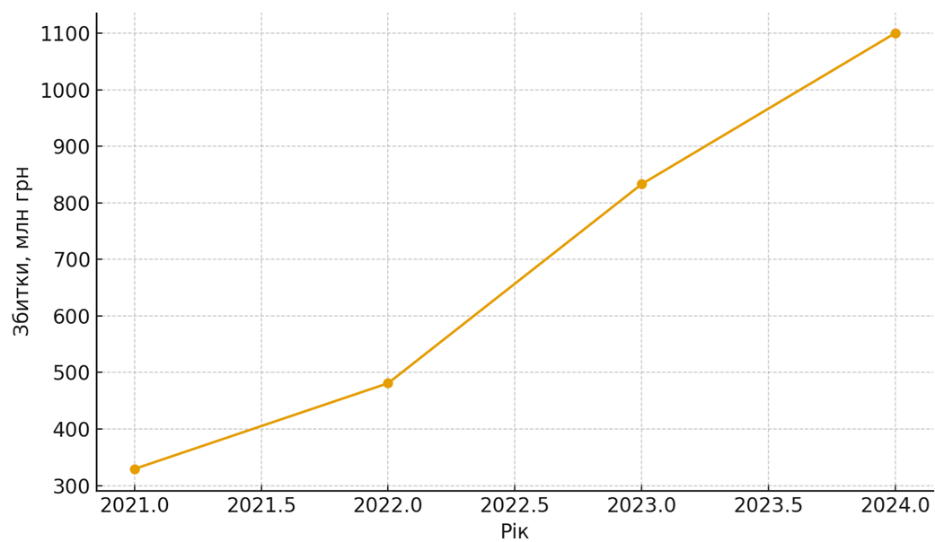
\includegraphics[width=0.9\linewidth]{img/figure1_1.png} 
    \caption{Збитки від шахрайств з платіжними картками в Україні}
    \label{fig:1_1}
\end{figure}

\newpage

На рис.~\ref{fig:1_1} показано лінійну динаміку збитків від незаконних дій з платіжними картками в Україні за 2021--2024~рр., яка була побудована автором на основі власних розрахунків та досліджень. Візуально видно рівень втрат, а подальше збільшення в 2024-му корелює з поширенням соціальної інженерії та зростанням середнього чека однієї незаконної операції. Це підтверджує ключову тезу розділу: шахрайство трансформувалося у системний бізнес, який базується не стільки на технічних вразливостях систем, скільки на маніпулюванні людським фактором і помилках користувачів~\cite{NBU2025}.

\vspace{0.3cm}
\section{Що найчастіше працює у шахраїв?}

Типові афери залишаються простими, але масовими. Найбільш поширені сценарії включають передоплату за товар, якого не існує, або «неймовірно вигідні» пропозиції від щойно створених акаунтів. Другою за масштабом схемою є сайти-двійники сервісу «OLX Доставка», які копіюють дизайн оригінальної сторінки й збирають реквізити карток під приводом «підтвердження доставки». 

А ще активно застосовуються цифрові псевдопослуги: фейкові страхування, оплата комуналки чи «швидкі кредити», де людина добровільно вводить персональні дані. Статистика демонструє, що вартість кожної атаки стрімко зростає. Середня сума шахрайської операції в інтернеті у 2024~році становила 4~761~грн, тоді як у 2023-му вона складала лише 3~150~грн. Більш того, у випадках довготривалого «ведення клієнта» (соціальна інженерія) шахраї виманювали в середньому 8~500~грн за одну оборудку. Це підтверджує, що шахрайство давно переросло дрібні випадкові крадіжки й перетворилося на бізнес-модель із власною економікою~\cite{NBU2025}.

\vspace{0.3cm}
\section{Чому люди «ведуться»?}

Зловмисники створюють ефект надпривабливості: пропозиція виглядає настільки вигідною, що мозок підсвідомо прагне уникнути втрати такого шансу. Далі активується штучний дефіцит часу: вимоги на кшталт «акція діє лише годину» або «підтвердіть оплату за 10 хвилин» блокують префронтальну кору, яка відповідає за логічний аналіз, і змушують діяти на рівні швидких реакцій. І нарешті, спрацьовує ефект соціального доказу: коли ми бачимо позитивний досвід інших у вигляді численних відгуків чи високих рейтингів (які часто є фальшивими), наш мозок автоматично маркує ситуацію як безпечну. Це нормальний еволюційний механізм орієнтації в соціумі, який шахраї використовують проти нас, щоб вимкнути раціональну перевірку фактів.

\chapter{Правова кваліфікація дій кібершахраїв}

Законодавство України передбачає комплексну відповідальність за шахрайські дії в цифровому просторі.

Згідно з Кримінальним кодексом України (ККУ), дії зловмисників кваліфікуються за кількома статтями залежно від методу вчинення злочину~\cite{CriminalCode}:

\begin{description}
    \item[ст. 190 (Шахрайство)] — заволодіння чужим майном або придбання права на майно шляхом обману чи зловживання довірою;
    
    \item[ст. 361] — несанкціоноване втручання в роботу інформаційних (автоматизованих), електронних комунікаційних мереж (застосовується у випадках технічного зламу або використання вразливостей систем);
    
    \item[ст. 361-1] — створення з метою протиправного використання, розповсюдження або збуту шкідливих програмних чи технічних засобів, а також їх розповсюдження;
    
    \item[ст. 361-2] — несанкціоновані збут або розповсюдження інформації з обмеженим доступом, яка зберігається в електронно-обчислювальних машинах (зокрема, бази даних платіжних карток, логінів та паролів).
\end{description}

\newpage

Окрім кримінального переслідування, важливу роль відіграють цивільно-правові наслідки використання чужих брендів, дизайнів та інтерфейсів для створення фішингових ресурсів. Цивільний кодекс України гарантує судовий захист прав інтелектуальної власності (ст.~432) та встановлює відповідальність за їх порушення (ст.~431)~\cite{CivilCode}.

\vspace{0.3cm}

Спеціальне законодавство деталізує ці норми:

\begin{enumerate}
    \item Закон України «Про охорону прав на знаки для товарів і послуг» визначає виключні права власника бренду (ст.~16) та кваліфікує як порушення будь-яке посягання на них, зокрема імітацію знаку або введення споживачів в оману (ст.~20)~\cite{LawTrademarks}.
    
    \item Для охорони елементів дизайну, текстів та зображень застосовується Закон України «Про авторське право і суміжні права». Він передбачає механізми припинення порушень та стягнення компенсації, а також визначає відповідальність власників вебсайтів за невидалення піратського контенту після отримання відповідної скарги~\cite{LawCopyright}.
    
    \item У випадках, коли шахрайський ресурс (клон) маскується під оригінальний сервіс, застосовуються норми Закону «Про захист від недобросовісної конкуренції» (ст.~15-1) щодо заборони поширення інформації, що вводить в оману~\cite{LawCompetition}.
\end{enumerate}

У судовій практиці для потерпілої сторони (наприклад, банку чи маркетплейсу) ключовим є доведення факту порушення прав інтелектуальної власності для застосування цивільних засобів захисту, що відбувається паралельно з фіксацією ознак шахрайства у межах кримінального провадження.

\vspace{0.3cm}
\noindent\textbf{Статистичні тенденції та висновки}

Порівняльний аналіз статистичних даних демонструє тривожну динаміку: від 481~млн гривень втрат у 2021~році до понад 1,1~млрд~грн у 2024-му. Це свідчить про те, що кібершахрайство перестало бути сукупністю поодиноких інцидентів і трансформувалося у системне явище, темпи розвитку якого випереджають ріст цифрової грамотності суспільства~\cite{NBU2025}.

У контексті платформ оголошень і псевдопослуг ключовою вразливістю є не слабкість технологій захисту, а людський фактор: надмірна довіра, поспіх та відсутність критичного мислення. 

За даними регулятора, саме соціальна інженерія стала причиною 93\% усіх фінансових втрат в інтернеті. Тут діє головне правило: чим привабливішою та «яскравішою» виглядає пропозиція, тим вища ймовірність, що це — ретельно підготовлена пастка~\cite{NBU2025}.

\chapter{Ознаки шахрайських пропозицій}

Найперший тригер\footnote{Первинний сигнал, який запускає настороженість і спонукає зупинитися та перевірити.} — занадто низька ціна або пропозиція, що виглядає «занадто вигідною». Шахраї навмисне ставлять вартість нижчу за ринкову, щоб спровокувати покупця діяти імпульсивно, наприклад демпінг\footnote{Від англ. dumping. Продаж товарів за цінами, нижчими від собівартості.} у 30--50\%. Коли людина бачить смартфон, ноутбук чи павербанк\footnote{Портативний зовнішній акумулятор, який дозволяє заряджати ваші електронні пристрої.} на третину дешевше, ніж у магазинах, мозок миттєво фіксує «вигоду» і відсуває сумніви на другий план (рис.~\ref{fig:1_2}). Технічно для шахрая це працює як приманка: оголошення створюється за кілька хвилин, а вже далі все тримається на психології довірливості. Кіберполіція України офіційно визначає цю ознаку як ключовий індикатор небезпеки. Правоохоронці застерігають: якщо ціна товару суттєво відрізняється від середньої ринкової ціни на аналогічні моделі (різниця понад 20--30\%), ймовірність шахрайства наближається до 100\%~\cite{CyberpoliceTips}.

% Параметр [H] змушує рисунок бути САМЕ ТУТ, а не <<десь на сторінці>>
\begin{figure}[H]
    \centering
    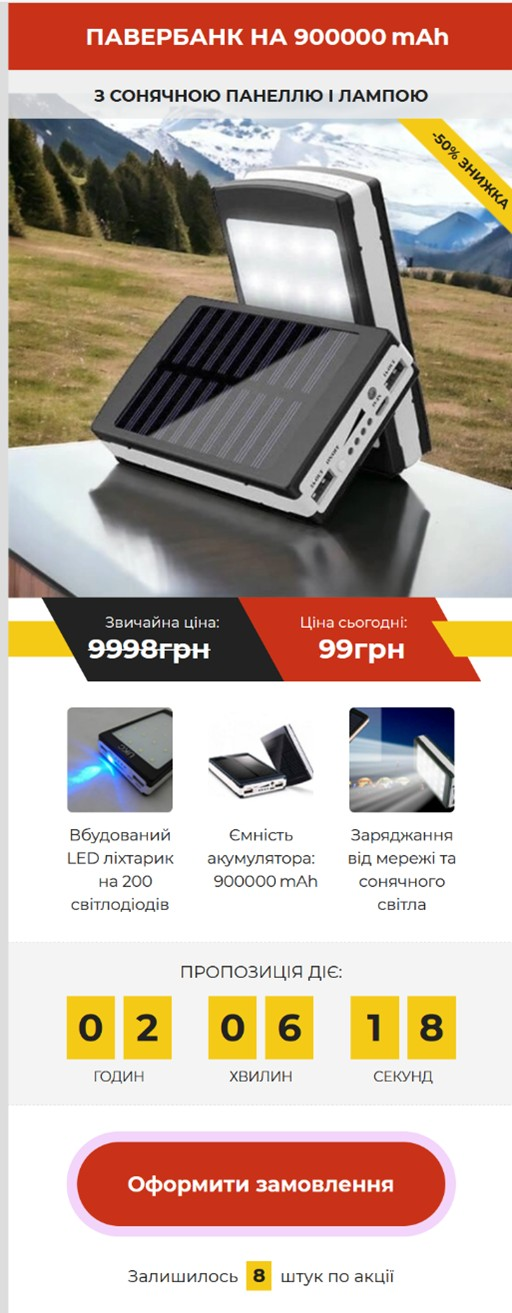
\includegraphics[width=0.50\linewidth]{img/figure1_2.jpg} 
    \caption{Приклад фейкової реклами на маркетплейсах}
    \label{fig:1_2}
\end{figure}

Зверніть увагу на технічні характеристики (рис.~\ref{fig:1_2}). Вказана на рекламному банері ємність у 900 000 mAh є фізично неможливою для пристрою такого розміру. 

Для порівняння: стандартний зовнішній акумулятор на 20 000 mAh важить близько 400–500 грамів. Повербанк ємністю 900 000 mAh мав би важити понад 15–20 кілограмів і за розмірами нагадував би автомобільний акумулятор або велику валізу. Використання таких «космічних» цифр — це пряма ознака шахрайства, розрахована на неуважність або технічну необізнаність покупця.

\vspace{0.3cm}
\noindent\textbf{Відсутність можливості зустрітися}

Ще однією характерною ознакою є відсутність можливості зустрітися особисто чи оглянути товар перед покупкою. Продавець знаходить «поважні причини»: мовляв, перебуває у відрядженні, товар зберігається на складі або він уже запакований для відправки. Така поведінка технічно дозволяє шахраю залишатися анонімним: йому не треба демонструвати фізичний товар, достатньо лише підтримувати контакт через месенджер. Це також спрощує використання фейкових фото, які легко взяти з інтернету.

\vspace{0.3cm}
\noindent\textbf{Вимога термінової передоплати}

Надзвичайно поширеним є прийом вимоги термінової передоплати. Класичне формулювання — «зараз або ніколи»: «ще кілька охочих чекають», «бронюю тільки після авансу». Тут шахрай використовує технічний інструмент — переказ на банківську картку чи електронний гаманець. У більш просунутих випадках надсилається покликання на підроблений сайт, що імітує платіжний сервіс. У цьому випадку користувач сам вводить дані своєї картки на фішинговій сторінці, після чого злочинець отримує прямий доступ до рахунку.

\vspace{0.3cm}

\newpage

\noindent\textbf{Некоректні або крадені фотографії}

Ще одна явна ознака — некоректні або крадені фотографії. Шахраї рідко мають справжній товар, тому беруть зображення з Google Images, Instagram чи офіційних сайтів виробників. Технічно це легко перевірити: достатньо завантажити фото в Google і знайти десятки ідентичних картинок у чужих оголошеннях. Це простий, але дієвий спосіб викрити шахрайство.

\vspace{0.3cm}
\noindent\textbf{Новостворений профіль}

Важливим показником є й новостворений профіль без історії чи з фейковими відгуками. Зловмисники відкривають акаунт, виставляють кілька «товарів», а щоб виглядати переконливо, підробляють коментарі — залишають штучні відгуки зі сторонніх акаунтів. Технічно це робиться через реєстрацію декількох профілів на один номер, через віртуальні SIM-карти чи тимчасові email-адреси (див. табл.~\ref{tab:table2}). Після того як профіль викривають і блокують, шахрай легко створює новий, повторюючи схему.

\newpage

\noindent Як це виглядає на практиці:


\begin{table}[H]
    \centering
    \caption{Маркери фейкових оголошень}
    \label{tab:table2}
    % Розподіл ширини колонок: 25%, 35%, 30% сторінки
    \begin{tabular}{|>{\raggedright\arraybackslash}p{0.23\linewidth}|>{\raggedright\arraybackslash}p{0.33\linewidth}|>{\raggedright\arraybackslash}p{0.28\linewidth}|}
        \hline
        \multicolumn{1}{|c|}{\textbf{Ознака}} & \multicolumn{1}{c|}{\textbf{Як працює технічно}} & \multicolumn{1}{c|}{\textbf{Чому діє психологічно}} \\ \hline
        
        Підозріло низька ціна & 
        Оголошення створюється з демпінгом (30--50\% від ринку), фото й опис беруться з інтернету & 
        Викликає відчуття «вигоди», знижує критичність, стимулює діяти швидко \\ \hline
        
        Відсутність зустрічі чи огляду & 
        Продавець вигадує причини: відрядження, склад, «товар запакований» & 
        Створює ілюзію раціональності: пояснення виглядають логічними і знижують пильність \\ \hline
        
        Вимога термінової передоплати & 
        Переказ на карту або покликання на фішинговий сайт, що імітує банк & 
        Тиск часу («зараз або ніколи») змушує приймати рішення імпульсивно \\ \hline
        
        Фейковi або чужi фотоо & 
        Зображення беруться з вiдкритих джерел & 
        Довіра до візуальних образів: якісні фото асоціюються з надійністю продавця \\ \hline
        
        Новостворений профіль без історії & 
        Реєстрацiя через тимчасовi данi, штучнi вiдгуки & 
        Маніпуляція соціальним доказом: створюється хибне відчуття безпечного середовища \\ \hline
    \end{tabular}
\end{table}

Таким чином, шахрайські пропозиції поєднують психологічний тиск (вигода, терміновість, довіра) з технічними прийомами (фейкові сайти, крадені фото, нові акаунти, підроблені відгуки). Для користувача важливо розуміти: якщо хоча б один із цих сигналів присутній, угоду варто перевіряти вдвічі ретельніше або взагалі відмовитися від неї.

Перевіряйте контакти таких покупців через спеціалізовані інструменти, наприклад GetContact або пошук у Google, а покликання — на VirusTotal, PhishTank (див. підрозділ~1.10).

\chapter{Інструменти для перевірки продавців та покупців}

Шахраї розраховують, що ви не перевірятимете. Перевірка — ваш найкращий щит.

\vspace{0.3cm}
\noindent\textbf{Чек-лист швидкої перевірки}

Щоб уникнути шахрайства під час онлайн-угод, головне правило – ніколи не здійснюйте передоплату незнайомим користувачам. Навіть невелика сума може бути втрачена, якщо оголошення фейкове. Безпечніше зустрітися особисто або скористатися оплатою при отриманні.

\vspace{0.3cm}
\noindent\textbf{Перевірка профілю}

Звертайте увагу на:
\begin{enumerate}
    \item \textbf{Дату реєстрації} — нові акаунти часто шахрайські.
    \item \textbf{Кількість і тематику оголошень} — якщо активність мінімальна або надто різнопланова, це сигнал ризику.
    \item \textbf{Відгуки} — реальні користувачі залишають конкретні коментарі, а не загальні «все добре».
    \item \textbf{Поведінку} — надмірна терміновість, надто вигідні умови чи готовність купити без огляду товару —  тригери обману.
\end{enumerate}

\newpage

\noindent\textbf{Перевірка зображень і контактів:}

\begin{enumerate}
    \item Перевіряйте фото товару через \textbf{Google Images}: якщо фото з’являється на інших сайтах, товар, ймовірно, неіснуючий.
    \item Шукайте номер телефону або email у \textbf{Google}, \textbf{Bing}, \textbf{WhoCallsMe.net}, \textbf{Truecaller.com} чи додатку \textbf{GetContact} — він часто показує, як інші користувачі зберегли цей номер («шахрай», «OLX доставка» тощо).
\end{enumerate}

\vspace{0.3cm}
\noindent\textbf{Перевірка платіжних реквізитів}

Якщо продавець просить передоплату, перевірте його картку через:
\begin{enumerate}
    \item \texttt{cyberpolice.gov.ua} — розділ «Stop Fraud» (або «Перевірити картку»).
    \item \texttt{ema.com.ua} (StopFraud) — база шахрайських рахунків.
    \item Перевірка IBAN на \texttt{bank.gov.ua} — дозволяє підтвердити належність рахунку банку.
\end{enumerate}

\vspace{0.3cm}
\noindent\textbf{Перевірка покликань}

Ніколи не переходьте за покликанням з месенджерів або SMS. Перевіряйте отримані URL\footnote{Текст зазвичай синього кольору, на який можна натиснути, щоб перейти на інший сайт.} через:
\begin{enumerate}
    \item \texttt{VirusTotal.com} — аналіз сайтів і файлів.
    \item \texttt{PhishTank.com} — база фішингових сторінок.
    \item \texttt{Whois.domaintools.com} — перевірка домену (дати реєстрації, власника).
\end{enumerate}

\newpage

Експерти Асоціації ЄМА наголошують: шахраї часто намагаються вивести спілкування з офіційної платформи в месенджери (Viber, Telegram), щоб надіслати фішингове покликання. Для перевірки будь-якого покликання, отриманого від продавця чи покупця, використовуйте сервіс \textbf{CheckMyLink} (\texttt{https://check.ema.com.ua/}).

Цей інструмент (рис.~\ref{fig:1_3}) перезвіряє покликання із загальноукраїнською базою шахрайських ресурсів та попереджає про небезпеку ще до моменту переходу на сайт~\cite{EMACheck}.

\begin{figure}[H]
    \centering
    % Переконайтеся, що файл називається fig1_3 (jpg/png) і лежить в папці img
    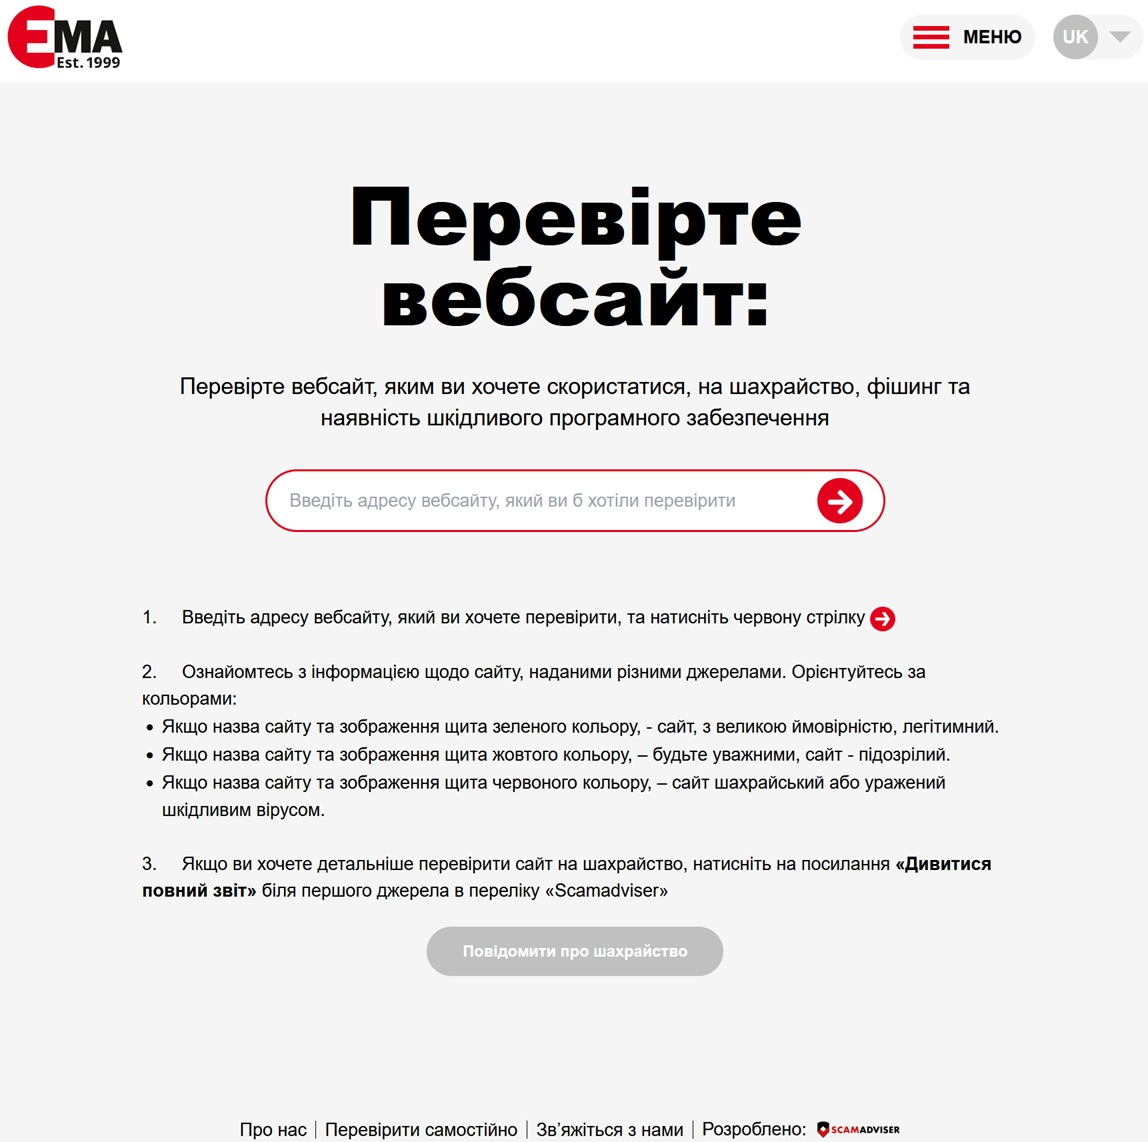
\includegraphics[width=0.75\linewidth]{img/figure1_3.jpg} 
    \caption{Вікно з перевіркою вебсайту на платформі ЄМА}
    \label{fig:1_3}
\end{figure}

Якщо сервіс показує, що сайт підозрілий або шахрайський, негайно припиніть спілкування.

\newpage

\chapter{Поради щодо захисту та дії у випадку шахрайства}

Безпечна угода — це не удача, а звичка. Щоб уникнути фінансових втрат і зберегти особисті дані, важливо не лише знати типові схеми шахраїв, а й діяти за чітким алгоритмом безпеки.

\section{Алгоритм безпечної угоди}

\vspace{0.3cm}
\noindent\textbf{Алгоритм безпечної угоди: як не стати жертвою шахраїв}

\begin{enumerate}
    \item \textbf{Всебічно перевіряйте контрагента.} Дивіться дату реєстрації профілю, кількість оголошень та відгуки (нові або «порожні» акаунти — сигнал ризику). Перевіряйте номер телефону, email або картку в Google, GetContact чи StopFraud. Зробіть зворотний пошук фото — якщо зображення крадені, це шахрай.
    
    \item \textbf{Користуйтеся лише офіційними сервісами.} Оплачуйте через вбудовані інструменти платформи (як «OLX Доставка») або інші надійні сервіси. Ніколи не переказуйте гроші напряму на картку невідомої особи.
    
    \item \textbf{Дотримуйтесь базової кібергігієни} (правила чистоти та безпеки в інтернеті). Увімкніть двофакторну автентифікацію (2FA), створюйте унікальні паролі та використовуйте окрему картку з лімітом для онлайн-платежів. Спілкуйтеся лише в офіційних чатах платформи.
    
\newpage

    \item \textbf{Вимагайте документи для дорогих покупок.} Для оренди чи купівлі нерухомості або авто вимагайте документи та звіряйте їх через офіційні державні реєстри.
    
    \item \textbf{Довіряйте здоровому глузду.} Якщо ціна занадто приваблива, продавець уникає дзвінків, поспішає або надто наполегливо вимагає передоплату — привід зупинити угоду. Якщо щось викликає сумнів — краще втратити можливу вигоду, ніж гроші та дані.
    
    \item \textbf{Зберігайте докази.} Якщо угода відбулася, збережіть усе: контакти, квитанції, чеки та повну історію листування.
\end{enumerate}

\section{Алгоритм дій. Що робити, якщо вас ошукали?}

Якщо ви зрозуміли, що передали дані шахраям або з вашого рахунку зникли гроші, ви можете відчути сильний сором, гнів або самозвинувачення. \textbf{Зупиніться.} Ваша реакція (паніка, прискорене серцебиття) є абсолютно нормальною відповіддю організму на гострий стрес. Пам’ятайте: те, що сталося — це результат застосування професійних технік психологічного тиску, а не ваша «провина» чи «наївність». Зараз час — ваш головний союзник, але діяти потрібно миттєво. Не дозволяйте емоціям заблокувати вашу рішучість. Поверніть собі контроль над ситуацією через ці чіткі кроки:

\begin{enumerate}
    \item \textbf{Заблокуйте банківську картку (НЕГАЙНО).}
    Це найперший крок, щоб шахраї не встигли зняти решту грошей.
    \begin{itemize}
        \item \textbf{Спосіб 1. Через мобільний застосунок.} Відкрийте програму вашого банку (Приват24, monobank, Ощад тощо) на телефоні. Знайдіть зображення вашої картки, натисніть на нього або на меню «Налаштування» (шестерня) і оберіть пункт \textbf{«Заблокувати картку»}.
   \newpage
   
        \item \textbf{Спосіб 2. Через гарячу лінію.} Якщо у вас немає застосунку або інтернету, терміново телефонуйте в банк.
        \item \textit{Де знайти номер?} Номер гарячої лінії завжди написаний \textbf{на зворотному боці вашої пластикової картки} (зазвичай починається на 0-800...). Також його можна знайти на офіційному сайті банку.
        \item \textit{Що казати?} «Я підозрюю шахрайство, терміново заблокуйте мої рахунки».
    \end{itemize}

    \item \textbf{Зверніться до банку офіційно.}
    Дзвінка недостатньо. Вам потрібно зафіксувати факт злочину документально.
    \begin{itemize}
        \item Зателефонуйте на гарячу лінію та повідомте оператору про крадіжку коштів.
        \item Вимагайте сформувати заявку на \textbf{повернення коштів} (процедура оскарження транзакції).
        \item Найближчим часом відвідайте відділення банку та напишіть письмову \textbf{заяву про несанкціоновану операцію}. Обов'язково попросіть копію цієї заяви з відміткою банку про отримання. Це ваш доказ для поліції та суду.
    \end{itemize}

    \item \textbf{Зберіть докази злочину.}
    Поки ви чекаєте на відповідь банку, збережіть усе, що стосується шахраїв. Потім вони можуть видалити листування.
    \begin{itemize}
        \item \textbf{Скріншоти (знімки екрана).} Сфотографуйте листування у месенджерах (Viber, Telegram), SMS-повідомлення, сторінку шахрайського сайту чи профілю продавця.
        \item \textbf{Фінансові дані.} Збережіть квитанції про переказ, номер картки, на яку ви скидали гроші, та точний час операції.
        \item \textbf{Контакти.} Запишіть номери телефонів, з яких вам дзвонили, та нікнейми (імена) шахраїв в інтернеті.
    \end{itemize}

    \item \textbf{Подайте заяву до Кіберполіції.}
    Не думайте, що «через 500 гривень ніхто не шукатиме». Ваша заява може стати частиною великої справи проти злочинної групи.
    \begin{itemize}
        \item \textbf{Варіант А (Онлайн, найшвидше).} Зайдіть на сайт Кіберполіції \url{https://ticket.cyberpolice.gov.ua/} та заповніть електронну форму «Повідомити про злочин».
        \item \textbf{Варіант Б (Особисто).} Підіть у найближче відділення поліції та напишіть заяву про вчинення кримінального правопорушення за статтею 190 ККУ (Шахрайство). Додайте до заяви роздруковані скріншоти та копії квитанцій.
    \end{itemize}
\end{enumerate}

\vspace{0.2cm}
\textit{\textbf{Пам'ятайте.} Банк ніколи не дзвонить, щоб запитати PIN-код, пароль від входу в кабінет або три цифри на звороті картки (CVV). Якщо вас про це запитують — це шахраї. Кладіть слухавку і дзвоніть у банк самі за номером на вашій картці.}

\clearpage            
%\input{main/chapter2.tex}            
%\input{main/chapter3.tex} 
%\input{main/chapter4.tex}  
%\input{main/chapter5.tex}  
%\chapter{Шкідливе програмне забезпечення та фейкові мобільні додатки}

% Ця команда примусово вирівнює текст по ширині, виправляючи помилки з попередніх розділів

У сучасному інформаційному просторі поняття «цифрова довіра» стає фундаментом безпечної взаємодії користувача з технологіями, адже ми звикли довіряти своїм смартфонам та комп’ютерам найцінніше — від особистих спогадів до доступу до банківських рахунків.

Довіра до інтерфейсу — це природний механізм економії когнітивних ресурсів нашого мозку. Саме на цій довірі паразитують кіберзлочинці, створюючи шкідливе програмне забезпечення та фейкові мобільні додатки. Вони не просто зламують пристрої, а зламують нашу біологічну здатність швидко орієнтуватися у звичному середовищі, імітуючи безпеку там, де її немає. Візуально копіюючи популярні сервіси чи корисні інструменти, такі програми мають на меті приховане викрадення даних або коштів. Руйнування цієї довіри не лише завдає прямих фінансових збитків, а й створює тривалий психологічний тиск на постраждалу особу, провокуючи вторинну травматизацію та змушуючи сумніватися в безпеці будь-яких цифрових послуг у майбутньому

Формування стійкої цифрової гігієни потребує не лише теоретичних знань, а й регулярного тренування у середовищі, максимально наближеному до реального. Саме такий підхід реалізовано в архітектурі навчальної платформи «Cyber Simulator», яка об’єднує всі розглянуті нами вектори загроз в єдину систему протидії.

\begin{figure}[H]
    \centering
    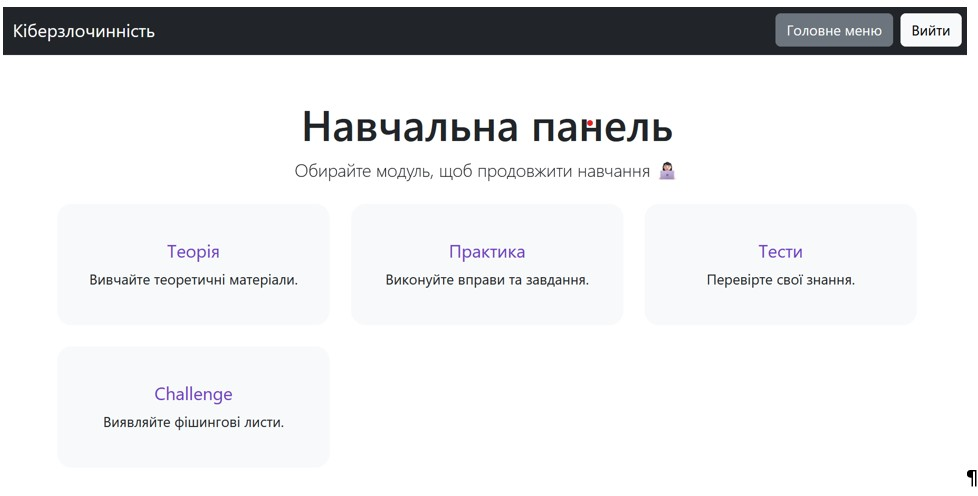
\includegraphics[width=0.98\linewidth]{img/figure6_1.jpg} 
    \caption{Інтерфейс головної панелі платформи для комплексного тренування навичок <<Cyber Simulator>>}
    \label{fig:6_1}
\end{figure}

Головна панель тренажера (рис.~\ref{fig:6_1}) надає користувачу швидкий доступ до симуляцій різних типів атак — від фішингу до SQL-ін’єкцій, дозволяючи візуалізувати власний прогрес та ідентифікувати слабкі місця у своїй системі знань.

\section*{Правова відповідальність}

Важливо усвідомлювати, що створення, використання та розповсюдження вірусів, троянів чи шпигунського програмного забезпечення — це не просто технічне хуліганство, а серйозна кримінальна діяльність, яка в Україні жорстко регулюється законом.

Дії зловмисників кваліфікуються за низкою статей Кримінального кодексу України~\cite{KKU2001}:
\begin{itemize}
    \item \textbf{Ст. 361.} Несанкціоноване втручання в роботу систем.
    \item \textbf{Ст. 361-1.} Створення та збут шкідливих програм.
    \item \textbf{Ст. 190.} Шахрайство.
\end{itemize}

Це означає, що за «легким заробітком» в інтернеті стоїть реальна кримінальна відповідальність. Правоохоронні органи мають інструменти для розслідування таких злочинів, спираючись як на національне законодавство, так і на міжнародну \textit{Конвенцію про кіберзлочинність}~\cite{Budapest_Convention_2001}.

Санкції за цими статтями передбачають суворе покарання, яке включає не лише значні штрафи та конфіскацію всіх програмних і технічних засобів, а й реальне позбавлення волі на тривалий термін.

\textit{\textbf{Важливо.} Окремо слід наголосити, що вчинення таких кіберзлочинів в умовах воєнного стану розглядається судом як обтяжуюча обставина, що значно посилює відповідальність. Тож розуміння природи шкідливого ПЗ потрібне не лише для захисту власних гаджетів, а й для усвідомлення правової межі, перетин якої перетворює користувача на злочинця.}

\section{Види шкідливих програм (віруси, трояни, шпигуни)}

\textbf{Шкідливе програмне забезпечення (ШПЗ, malware)} — це будь-які програми або код, створені з метою завдати шкоди користувачу, пристрою чи системі. Вони можуть блокувати роботу пристрою, викрадати дані або надавати зловмисникам несанкціонований доступ.

\vspace{0.3cm}

До основних типів шкідливих програм належать:

\begin{enumerate}
    \item \textbf{Програми-вимагачі (Ransomware).}
    Шкідливе ПЗ, яке шифрує або блокує файли й вимагає викуп за їх розблокування.
    \newline \textit{Приклад:} \textbf{WannaCry (2017)} — швидко зашифрував файли сотень тисяч ПК і вимагав платіж у біткоїнах.  

 \newpage

    \item \textbf{Трояни (Trojans).}
    Використовують візуальну ідентичність відомих брендів для вимкнення критичного сприйняття користувача, щоб непомітно виконувати шкідливі дії (приховано збирати персональні дані, перехоплювати управління пристроєм).
    \newline \textit{Приклад:} \textbf{Zeus} — перехоплював логіни в онлайн-банкінгу й виконував неавторизовані перекази.

    \item \textbf{Хробаки (Worms).}
    Поширюються мережею або через носії без участі користувача, часто викликають масові збої.
    \newline \textit{Приклад:} \textbf{SQL Slammer} — за кілька хвилин спричинив масштабні проблеми в мережах.

    \item \textbf{Рекламне ПЗ (Adware).}
    Нав’язливо показує рекламу, може перенаправляти на шахрайські сайти або змінювати налаштування браузера.
    \newline \textit{Приклад:} Кампанія \textbf{Fireball (2017)} — змінила стартові сторінки мільйонів комп'ютерів.

    \item \textbf{Ботнети\footnote{Мережа заражених пристроїв («зомбі»), якими керують зловмисники для виконання різних атак та злочинних дій.} (Botnets).}
    Мережі заражених пристроїв («зомбі»), якими керують зловмисники для DDoS-атак, розсилок або інших злочинних дій.
    \newline \textit{Приклад:} \textbf{Mirai (2016)} — DDoS-атаки з інфікованих IoT-пристроїв вивели з ладу великі сервіси. 

    \item \textbf{Шпигунське ПЗ (Spyware).}
    Непомітно збирає дані з пристрою: натискання клавіш, логіни й паролі, історію браузера, cookies, геолокацію, а інколи — аудіо чи відео; використовується для крадіжки облікових даних, банківської інформації або стеження. Основною метою цього класу програм залишається викрадення облікових даних та банківської інформації.
    
    Згідно з аналітичними даними компаній Check Point та Symantec, у 2023–2024 роках частка мобільного шпигунського ПЗ у загальній структурі шкідливих програм зросла з 12\% до 15\%. Експерти пов'язують цей тренд з еволюцією банківських троянів, які дедалі частіше інтегрують у себе шпигунські модулі для тотального контролю над інфікованим смартфоном~\cite{CheckPoint_2024, Symantec_Threat_2024}.

    \item \textbf{Руткіти\footnote{Програми, що надають зловмиснику прихований адміністративний доступ до системи та маскують свою присутність.} (Rootkits).}
    Програми, що надають зловмиснику прихований адміністративний доступ до системи. Відрізняються здатністю маскувати власну присутність та інше шкідливе ПЗ, що ускладнює виявлення.
    \newline \textit{Приклад:} \textbf{Stuxnet (2010)} — використовував руткіт-компоненти для приховування своєї присутності на заражених промислових системах.
\end{enumerate}

\subsection*{Ландшафт загроз 2024 року: Статистика та фінанси}

У 2024 році ландшафт кіберзагроз характеризувався чітким домінуванням шкідливого програмного забезпечення, орієнтованого на прихований контроль та прямий шантаж.

Статистичний аналіз інцидентів дозволяє виділити наступну структуру атак~\cite{AnyRun_Malware_2024}:

\begin{enumerate}
    \item \textbf{Троянські програми (Trojans).}
    Беззаперечний лідер загроз — зафіксовано близько \textbf{18 000} випадків, що становить \textbf{32\%} від загальної кількості атак. Це свідчить про те, що маскування під легітимне ПЗ залишається найефективнішим методом проникнення.

    \item \textbf{Програми-вимагачі (Ransomware).}
    Посіли друге місце з показником понад \textbf{12 000} інцидентів (\textbf{22\%}). Разом із троянами ці дві категорії сформували більше половини (54\%) усього вектора загроз.

    \item \textbf{Шпигунське ПЗ (Spyware).}
    Виявило значну активність — близько \textbf{9 000} випадків (\textbf{16\%}).
\end{enumerate}

Для розуміння природи загроз та методів протидії їм наведено детальну класифікацію шкідливого ПЗ (див. табл.~\ref{tab:table6_1}).

\begin{table}[H]
    \centering
    \footnotesize
    \caption{Класифікація шкідливого програмного забезпечення та особливості його роботи}
    \label{tab:table6_1}
    \renewcommand{\arraystretch}{1.05}
    \begin{tabular}{|>{\raggedright\arraybackslash}p{0.30\linewidth}|>{\raggedright\arraybackslash}p{0.30\linewidth}|>{\raggedright\arraybackslash}p{0.30\linewidth}|}
        \hline
        \multicolumn{1}{|c|}{\shortstack{\textbf{Вид шкідливого} \\ \textbf{ПЗ}}} & \multicolumn{1}{c|}{\shortstack{\textbf{Технічна} \\ \textbf{характеристика}}} & \multicolumn{1}{c|}{\shortstack{\textbf{Особливості} \\ \textbf{роботи}}} \\
        \hline
        \textbf{Програми-вимагачі} & Шифрування або блокування файлів системи & Монетизація через викуп (часто криптовалюта) \\
        \hline
        \textbf{Трояни} & Створення прихованого доступу (backdoor), крадіжка даних, доставка іншого ШПЗ & Маскування під легітимне ПЗ. Використовує механізми соціальної інженерії для стимулювання дії користувача \\
        \hline
        \textbf{Хробаки} & Перевантаження мережі, масове зараження & Самопоширення через мережеві вразливості. Не потребує дій користувача \\
        \hline
        \textbf{Рекламне ПЗ} & Показ нав'язливої реклами, редиректи, збір статистики & Встановлюється (часто приховано) разом з іншою програмою, яка завантажується \\
        \hline
    \end{tabular}
\end{table}



\begin{table}[H]
    \centering
    \footnotesize
    \caption*{Продовження таблиці 6.1}
    \renewcommand{\arraystretch}{1.05}
    \begin{tabular}{|>{\raggedright\arraybackslash}p{0.30\linewidth}|>{\raggedright\arraybackslash}p{0.30\linewidth}|>{\raggedright\arraybackslash}p{0.30\linewidth}|}
        \hline
        \multicolumn{1}{|c|}{\shortstack{\textbf{Вид шкідливого} \\ \textbf{ПЗ}}} & \multicolumn{1}{c|}{\shortstack{\textbf{Технічна} \\ \textbf{характеристика}}} & \multicolumn{1}{c|}{\shortstack{\textbf{Особливості} \\ \textbf{роботи}}} \\
        \hline
        \textbf{Ботнети} & Виконання команд (DDoS, спам, майнінг) & Централізоване управління мережею заражених пристроїв (зомбі-пристрої) \\
        \hline
        \textbf{Шпигунське ПЗ} & Крадіжка конфіденційної інформації (кейлоггінг, скріншоти, дані камери) & Прихована робота у фоновому режимі, моніторинг активності \\
        \hline
        \textbf{Віруси} & Пошкодження або модифікація файлів & Ін'єкція коду у легітимні файли. Потребує запуску файлу-носія для поширення \\
        \hline
        \textbf{Руткіти} & Надання повного (адміністративного) доступу до системи & Приховування присутності на рівні ядра ОС. Маскує файли, процеси та з'єднання \\
        \hline
    \end{tabular}
\end{table}

\textbf{Мобільний сегмент}
Окремий тренд спостерігається у мобільному сегменті: рекламне ПЗ (\textit{Adware}) та фейкові додатки сумарно охопили \textbf{21\%} ринку загроз (7 000 та 5 000 випадків відповідно). Менш чисельними, але стабільними загрозами залишилися ботнети (4 000) та комп'ютерні черв'яки (3 000), тоді як на специфічні інструменти (руткіти, криптоджекери) припало близько 4\% інцидентів.


\subsection*{Фінансовий моніторинг наслідків}

Фінансовий моніторинг наслідків кіберактивності у 2024 році демонструє чітку ієрархію загроз за рівнем монетизації.

\begin{itemize}
    \item \textbf{Ransomware.} Безумовний лідер за обсягом завданих збитків. Програми-вимагачі продемонстрували загрозливу динаміку зростання: щомісячні втрати постраждалих користувачів збільшилися майже вдвічі — з \$850 млн у січні до понад \textbf{\$1,5 млрд} у грудні.

    \item \textbf{Trojans.} Другу позицію у рейтингу фінансових загроз посіли троянські програми. Пік їхньої активності припав на серпень, коли сумарні збитки сягнули \textbf{\$1,25 млрд}, що пояснюється сезонними сплесками фішингових кампаній та відпустками персоналу служб безпеки.

    \item \textbf{Spyware.} Стабільно високий рівень фінансових втрат генерувало шпигунське ПЗ, збитки від якого наприкінці року оцінювалися в діапазоні \textbf{\$500--550 млн} щомісяця.

    \item \textbf{Фейкові мобільні додатки.} Аналітики відзначають тривожний тренд: якщо на початку року втрати становили \$180 млн, то у грудні цей показник зріс до \textbf{\$310 млн}, що корелює зі зростанням популярності мобільного банкінгу.
\end{itemize}



Інші вектори атак (рекламне ПЗ, черв'яки, ботнети), хоча й мали менший руйнівний потенціал, забезпечували постійний фон фінансових втрат у діапазоні \$100--300 млн на місяць.

\vspace{0.3cm}
\textit{Наведені оцінки базуються на крос-аналізі даних провідних галузевих звітів за 2024 рік: Check Point Cyber Security Report, Symantec Threat Landscape Report, Europol IOCTA, Chainalysis Crypto Crime Report~\cite{CheckPoint_2024, Symantec_Threat_2024, Europol_IOCTA_2024, Chainalysis_Crypto_2024}.}

Різні типи вірусів використовують специфічні канали проникнення та мають свої пріоритетні мішені; цей взаємозв'язок деталізовано в таблиці~\ref{tab:table6_2}.

\begin{table}[H]
    \centering
    \footnotesize
    \caption{Вектори поширення та типові цілі шкідливого програмного забезпечення}
    \label{tab:table6_2}
    \renewcommand{\arraystretch}{1.05}
    \begin{tabular}{|>{\raggedright\arraybackslash}p{0.30\linewidth}|>{\raggedright\arraybackslash}p{0.30\linewidth}|>{\raggedright\arraybackslash}p{0.30\linewidth}|}
        \hline
        \multicolumn{1}{|c|}{\shortstack{\textbf{Вид шкідливого} \\ \textbf{ПЗ}}} & \multicolumn{1}{c|}{\shortstack{\textbf{Основні вектори} \\ \textbf{атаки}}} & \multicolumn{1}{c|}{\shortstack{\textbf{Типові} \\ \textbf{цілі}}} \\
        \hline
        \textbf{Програми-вимагачі} & Email-вкладення, експлойти\footnotemark[3]\ вразливостей, RDP-атаки\footnotemark[4], фішингові сайти & Великі організації, лікарні, муніципальні установи, критична інфраструктура \\
        \hline
        \textbf{Трояни} & Фішингові листи, завантаження з веб-сайтів, зламані програми, оновлення софту & Банківські дані, облікові записи, бізнес-інформація, особисті файли \\
        \hline
        \textbf{Хробаки} & Експлуатація мережевих вразливостей, USB-накопичувачі, незахищені мережеві порти & Корпоративні мережі, IoT-пристрої, застарілі системи без оновлень \\
        \hline
        \textbf{Рекламне ПЗ} & Bundling\footnotemark[5]\ з безкоштовним ПЗ, браузерні розширення, оманливі банери & Пересічні користувачі, власники веб-сайтів, онлайн-рекламодавці \\
        \hline
    \end{tabular}
\end{table}
\footnotetext[3]{Код для використання вразливостей системи.}
\footnotetext[4]{Атаки через протокол віддаленого робочого столу.}
\footnotetext[5]{Об'єднання кількох програм в один інсталяційний пакет.}

\begin{table}[H]
    \centering
    \footnotesize
    \caption*{Продовження таблиці 6.2} 
    \renewcommand{\arraystretch}{1.05}
    \begin{tabular}{|>{\raggedright\arraybackslash}p{0.30\linewidth}|>{\raggedright\arraybackslash}p{0.30\linewidth}|>{\raggedright\arraybackslash}p{0.30\linewidth}|}
        \hline
        \multicolumn{1}{|c|}{\shortstack{\textbf{Вид шкідливого} \\ \textbf{ПЗ}}} & \multicolumn{1}{c|}{\shortstack{\textbf{Основні вектори} \\ \textbf{атаки}}} & \multicolumn{1}{c|}{\shortstack{\textbf{Типові} \\ \textbf{цілі}}} \\
        \hline
        \textbf{Ботнети} & Заражені IoT-пристрої, брутфорс\footnotemark[6]\ паролів, експлойти маршрутизаторів & DDoS-атаки на сервіси, розсилка спаму, криптомайнінг \\
        \hline
        \textbf{Шпигунське ПЗ} & Підроблені мобільні додатки, зламані програми, фішинг, уразливості нульового дня\footnotemark[7] & Журналісти, активісти, політики, бізнес-конкуренти, приватні особи \\
        \hline
        \textbf{Віруси} & Email-вкладення, заражені документи Office, інфіковані USB-накопичувачі & Файли користувачів, системні файли, документи, мережеві ресурси \\
        \hline
        \textbf{Руткіти} & Експлойти операційних систем, зламані драйвери, фізичний доступ до системи & APT-атаки\footnotemark[8]\ на уряди, промислові системи, критична інфраструктура \\
        \hline
    \end{tabular}
\end{table}
\footnotetext[6]{Метод підбору паролів перебором усіх варіантів.}
\footnotetext[7]{Невідомі розробникам вразливості без виправлень.}
\footnotetext[8]{Тривалі цілеспрямовані кібератаки організованих груп.}

Щоб оцінити реальний масштаб проблеми та виявити домінуючі тенденції, проаналізуємо структуру кіберінцидентів за останній звітний період (див. рис.~\ref{fig:6_2}).

\begin{figure}[H]
    \centering
    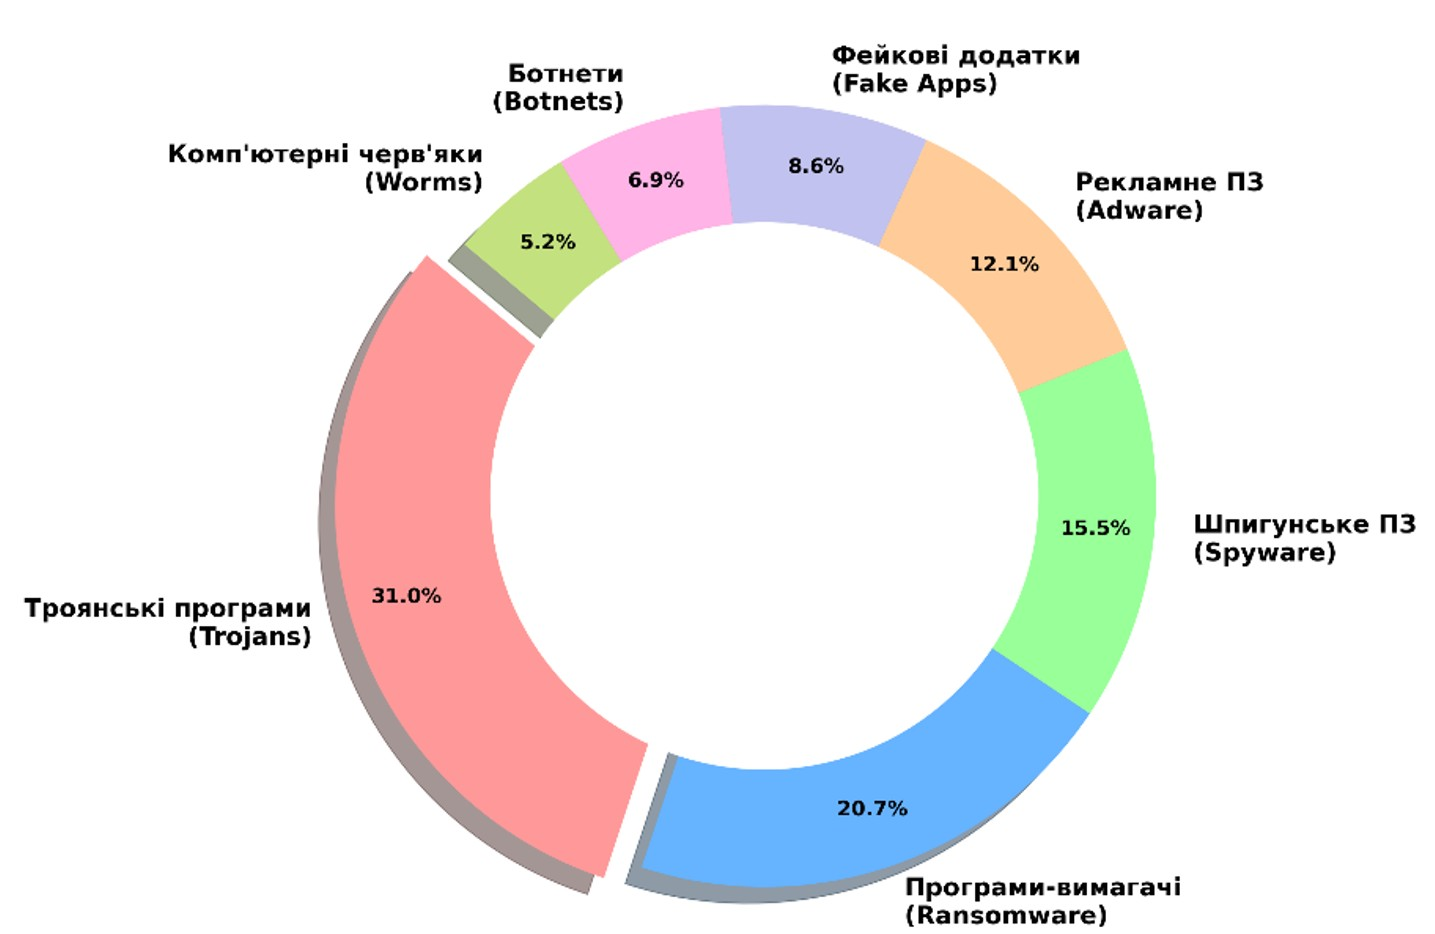
\includegraphics[width=0.90\linewidth]{img/figure6_2.jpg} 
    \caption{Структура кіберзагроз у 2024 році (розподіл за кількістю інцидентів)}
    \label{fig:6_2}
\end{figure}

\subsection*{Правова кваліфікація дій}

Правова кваліфікація дій, пов’язаних із розробкою та розповсюдженням шкідливого програмного забезпечення (зокрема фейкових мобільних додатків), в Україні здійснюється на основі норм Кримінального кодексу України (ККУ) та ратифікованих міжнародних договорів~\cite{KKU2001}.

До ключових статей, що інкримінуються у справах про кіберзлочини, належать:

\begin{description}
    \item[Ст. 361 ККУ.] «Несанкціоноване втручання в роботу інформаційних (автоматизованих), електронних комунікаційних, інформаційно-комунікаційних систем, електронних комунікаційних мереж». Ця стаття є базовою для кваліфікації злому систем та крадіжки даних.

    \newpage

    \item[Ст. 361-1 ККУ.] «Створення з метою протиправного використання, розповсюдження або збуту шкідливих програмних чи технічних засобів, а також їх розповсюдження або збут». Вона безпосередньо стосується розробників вірусів, троянів та програм-вимагачів.

    \item[Ст. 190 ККУ.] «Шахрайство». Застосовується (зокрема ч. 3 та ч. 4) у випадках заволодіння чужим майном шляхом обману з використанням електронно-обчислювальної техніки.

    \item[Ст. 200 ККУ.] «Незаконні дії з документами на переказ, платіжними картками та іншими засобами доступу до банківських рахунків». Ця норма регулює злочини у сфері електронного банкінгу (кардинг, скімінг).
\end{description}

Санкції за цими статтями передбачають значні штрафи, конфіскацію програмних та технічних засобів, а також позбавлення волі. Варто зазначити, що вчинення цих злочинів під час \textbf{воєнного стану} розглядається як обтяжуюча обставина.

Інтеграцію України у світову систему безпеки забезпечує \textit{Конвенція про кіберзлочинність} (Будапештська конвенція, 2001), ратифікована Верховною Радою у 2005 році. Цей документ уніфікує підходи до криміналізації розробки шкідливого ПЗ та створює правову основу для транскордонної співпраці правоохоронних органів у розслідуванні інтернет-злочинів~\cite{Budapest_Convention_2001}.


\section{Канали поширення через додатки та файли}

Канали поширення — це способи, якими шкідливе програмне забезпечення (ШПЗ) та фейкові мобільні додатки потрапляють на пристрої користувачів.

\newpage

До основних каналів належать:

\begin{enumerate}
    \item \textbf{Електронна пошта та веб-додатки.}
    Зараження через підозрілі покликання (фішинг) або шкідливі вкладення.

    \item \textbf{Завантаження з неофіційних джерел (Sideloading).}
    Встановлення мобільних додатків не з офіційних магазинів (Google Play, Apple App Store, Microsoft Store), а з веб-сайтів, форумів чи файлообмінників. Це основний шлях для потрапляння неперевіреного коду на пристрій.

    \item \textbf{Піратське ПЗ.}
    Розповсюдження «зламаних» (cracked) версій платних програм або інсталяторів, які маскуються під легітимне ПЗ, але модифіковані зловмисниками для прихованого встановлення вірусів.

    \item \textbf{Рекламні мережі (Malvertising).}
    Сторінки, які при перегляді веб-контенту автоматично перенаправляють користувача на небезпечні ресурси або завантажують шкідливий код.

    \item \textbf{Автоматичне зараження (Drive-by downloads).}
    Відбувається приховано під час відвідування скомпрометованого (легального, але зламаного) або спеціально створеного шахрайського веб-сайту.
\end{enumerate}

Такий поділ допомагає зрозуміти, якими шляхами зловмисники поширюють шкідливе ПЗ та на що слід звертати увагу.

\subsection*{Вектори атак у 2024 році}

У 2024 році архітектура вхідних точок для кібератак продемонструвала чітку специфіку залежно від сектору.

\newpage

\textbf{1. Корпоративний сектор}
Згідно зі звітом \textit{Verizon Data Breach Investigations Report (DBIR) 2024}, веб-додатки та електронна пошта залишаються головними векторами проникнення. Аналітики підкреслюють, що успішні атаки на веб-інтерфейси найчастіше реалізуються через два механізми: експлуатацію технічних вразливостей ПЗ або використання викрадених облікових даних \textit{<<Credential Stuffing>>} ~\cite{Verizon_DBIR_2024}.

\textbf{2. Мобільний сегмент}
Тут ключовою проблемою залишається завантаження програм із неофіційних джерел (\textit{sideloading}).

\begin{itemize}
    \item \textbf{Масштаб загрози.} За даними Google, система безпеки \textit{Google Play Protect} у 2024 році виявила понад \textbf{13 мільйонів} нових шкідливих застосунків, які намагалися встановитися поза межами офіційного магазину.
    \item \textbf{Джерело інфекції.} Статистика підтверджує небезпеку сторонніх джерел: понад \textbf{95\%} встановлень шкідливих програм, які зловживають критичними дозволами (доступ до SMS, контактів, фінансів), відбувалися через веб-браузери, файлові менеджери або месенджери, а не через Google Play Store~\cite{Google_BadApps_2024}.
    \item \textbf{Реакція екосистеми.} Протягом року Google заблокував публікацію 2,36 млн застосунків, що порушували політики безпеки, та забанив понад 158 000 акаунтів недобросовісних розробників.
\end{itemize}

Оскільки смартфони стали основними носіями конфіденційної інформації, зловмисники фокусують увагу саме на них. Візуалізацію ландшафту загроз для мобільних платформ наведено на рис.~\ref{fig:6_3}.

\begin{figure}[H]
    \centering
    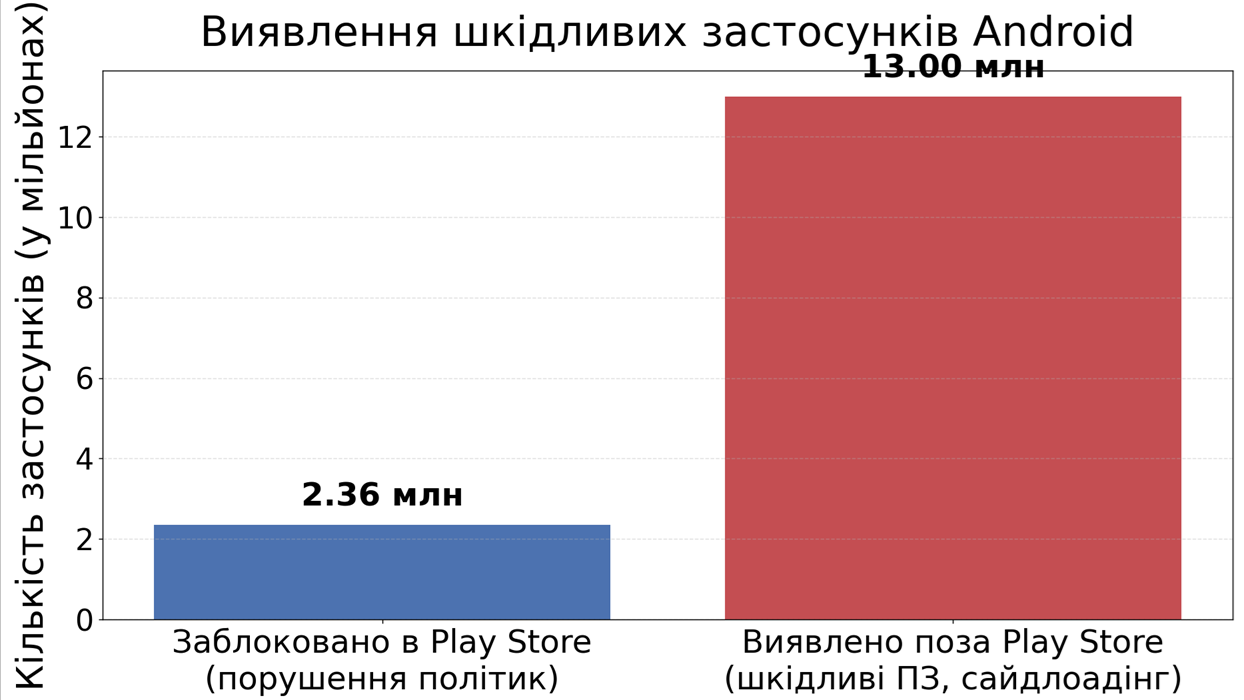
\includegraphics[width=0.99\linewidth]{img/figure6_3.png} 
    \caption{Візуалізація на мобільні пристрої)}
    \label{fig:6_3}
\end{figure}

\subsection*{Глобальний моніторинг: загрози sideloading}

Глобальний моніторинг мобільної безпеки підтверджує, що інсталяція додатків в обхід офіційних магазинів (\textit{sideloading}) є системною вразливістю екосистеми Android. Згідно зі звітом Zimperium «Global Mobile Threat Report 2024», саме цей вектор є джерелом значної частини інцидентів~\cite{Zimperium_Mobile_2024}.



\textbf{Географічний аналіз.}
Аналіз показує критичну ситуацію в Азійсько-Тихоокеанському регіоні, де близько \textbf{43\%} мобільних пристроїв мали встановлені застосунки з неофіційних джерел. Це створює сприятливе середовище для поширення:
\begin{itemize}
    \item мобільного шкідливого ПЗ (\textit{malware});
    \item рекламних вірусів (\textit{adware});
    \item кампаній з примусового встановлення небажаного софту.
  \end{itemize}

\newpage

\textbf{Масштаби протидії.}
Масштаби протидії цим загрозам ілюструють показники роботи системи \textit{Google Play Protect}: алгоритми захисту щодня сканують понад \textbf{200 мільярдів} застосунків, виконуючи глибинний аналіз на рівні коду для виявлення поліморфних загроз ще до їх активації на пристрої користувача (див. рис.~\ref{fig:6_4}).

\begin{figure}[H]
    \centering
    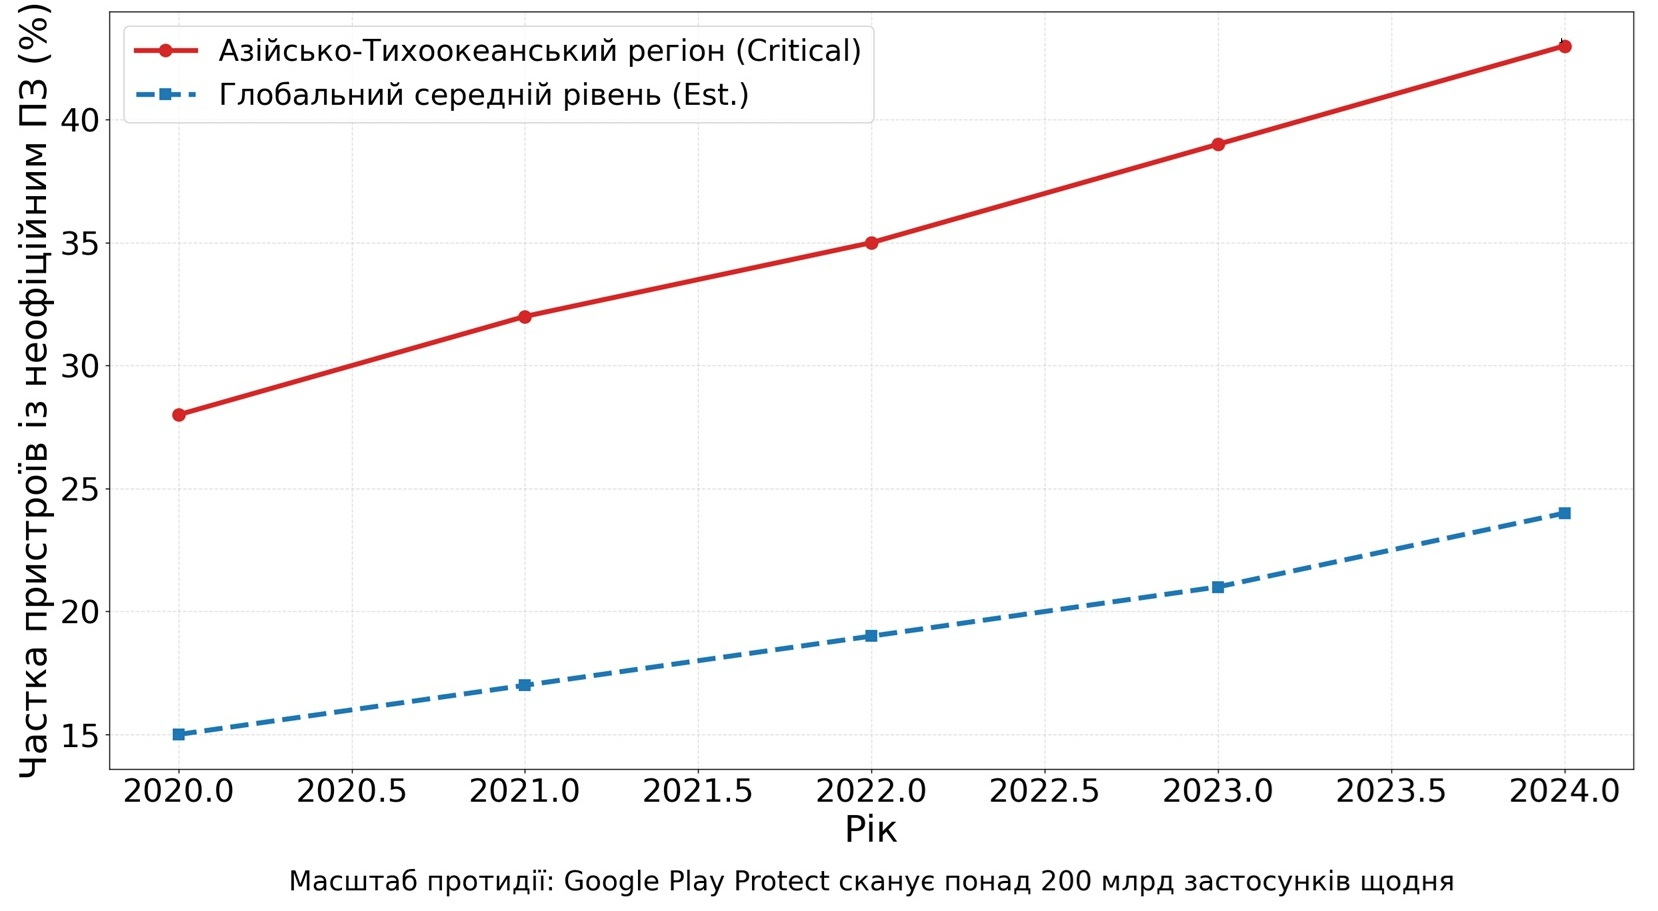
\includegraphics[width=0.90\linewidth]{img/figure6_4.jpg} 
    \caption{Динаміка вразливості екосистеми Android: Sideloading(Інсталяція додатків в обхід офіційних магазинів)}
    \label{fig:6_4}
\end{figure}

На рис.~\ref{fig:6_4} показано, звідки йдуть найбільші ризики. Щоб уникати їх, необхідно дотримуватися суворої цифрової гігієни:

\begin{itemize}
    \item \textbf{Не завантажувати} файли з підозрілих сайтів (особливо «зламані» програми).
    \item \textbf{Не відкривати} сумнівні покликання в SMS та чатах (навіть від знайомих).
    \item \textbf{Не відкривати} незнайомі вкладення в електронній пошті (архіви, офісні документи).
    \item \textbf{Не підключати} невідомі USB-накопичувачі до свого комп'ютера.
\end{itemize}

\newpage

Зловмисники адаптують свої інструменти під специфіку різних операційних систем. Співвідношення векторів поширення шкідливого ПЗ та їхніх цільових платформ показано на рис.~\ref{fig:6_5}.

\begin{figure}[H]
    \centering
    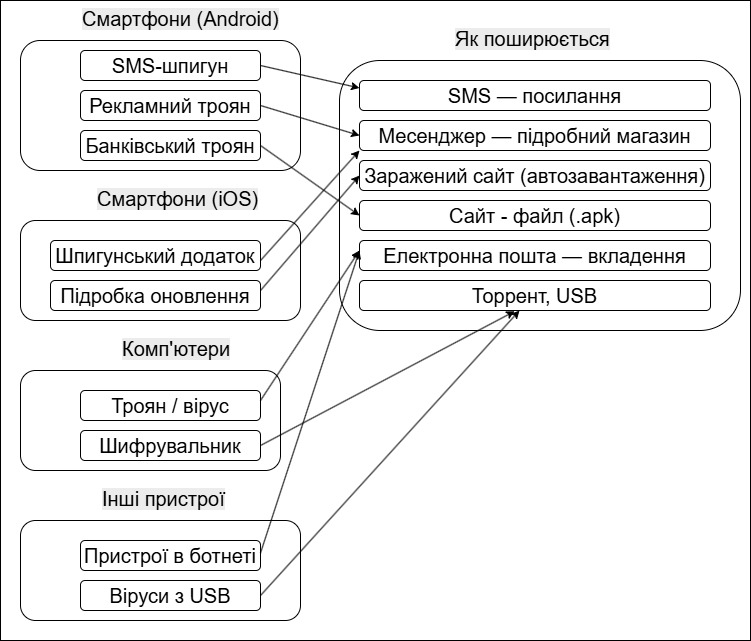
\includegraphics[width=0.80\linewidth]{img/figure6_5.jpg} 
    \caption{Вектори поширення шкідливого ПЗ та їх цільові платформи)}
    \label{fig:6_5}
\end{figure}

На схемі (див. рис.~\ref{fig:6_5}) показано, які пристрої найчастіше піддаються шкідливому ПЗ, які програми це ПЗ представляє і як воно потрапляє до користувачів.

\vspace{0.3cm}

\textbf{Структура схеми:}
\begin{itemize}
    \item \textbf{Зліва} позначені групи пристроїв: смартфони на Android, смартфони на iOS, комп’ютери та інші пристрої.
    \item \textbf{У середній частині} наведено приклади шкідливих програм для кожної групи — наприклад, банківські трояни, SMS-шпигуни, рекламні трояни, шифрувальники, віруси.

\newpage

    \item \textbf{Праворуч} показані звичайні шляхи поширення: завантаження файлів із веб-сайтів (\texttt{.apk} для Android), шкідливі покликання в SMS або чатах, підробні магазини додатків, вкладення в електронній пошті, торрент-файли, USB-накопичувачі та заражені сайти з автозавантаженням.
\end{itemize}

Стрілки на схемі ілюструють, який тип загрози найчастіше поширюється через конкретний канал — наприклад, банківський троян зазвичай приходить через файл із сайту, SMS-шпигун — через покликання в повідомленні, а шифрувальник — через піратські інсталятори або вкладення в листі.

\subsection*{Специфіка загроз за типом пристрою}

\begin{description}
    \item[Android-смартфони.]
    Основні загрози — банківські трояни, SMS-шпигуни та рекламні трояни. Вони поширюються переважно через неофіційні джерела: пряме завантаження \texttt{.apk} із сайтів, покликання у SMS або через підробні магазини додатків у месенджерах.

    \item[Смартфони на iOS.]
    Хоч і більш закриті, вони вразливі до шпигунських додатків та підроблених оновлень, які потрапляють через підробні магазини (з вимогою встановлення корпоративних профілів) або заражені веб-сайти з автоматичним завантаженням (\textit{drive-by}).

    \item[Комп’ютери.]
    Залишаються ціллю класичних троянів і вірусів, що найчастіше потрапляють через вкладення в електронній пошті. Шифрувальники та інше шкідливе ПЗ також активно поширюються через торрент-трекери або фізичні носії, такі як USB.
\end{description}

\section{Як працюють фейкові мобільні застосунки}

\textbf{Фейкові мобільні додатки} — це програми, які виглядають як знайомі сервіси (банк, маркетплейс, служба доставки або месенджер), але зроблені шахраями, щоб вкрасти ваші дані або гроші.

Вони копіюють логотипи й інтерфейс, щоб викликати довіру, і через це люди вводять логін, пароль або дані картки, думаючи, що користуються офіційною програмою.

\textbf{Механіка атаки.}
Всередині такі додатки приховують зловмисний код:
\begin{itemize}
    \item можуть показувати підробні вікна поверх справжніх банківських програм (так звані \textit{оверлеї});
    \item читати SMS з одноразовими кодами;
    \item збирати контакти та журнал дзвінків або відправляти інформацію на сервер шахраїв;
    \item іноді вони також запускають рекламу або використовують ресурси телефону для майнінгу (\textit{криптоджекінг}).
\end{itemize}

\subsection*{Як захиститися?}

Щоб не потрапити на шахраїв, дотримуйтесь наступних правил:
\begin{enumerate}
    \item \textbf{Завантажуйте програми тільки з офіційних магазинів} (Google Play, App Store).
    \item \textbf{Перевіряйте} ім’я розробника і відгуки перед встановленням.
    \item \textbf{Уважно дивіться}, які права (дозволи) просить додаток.
    \item \textbf{Не переходьте} за підозрілими покликаннями з SMS, чатів.
    \item \textbf{Використовуйте} мобільний захист (антивірус) за потреби.
\end{enumerate}

Для кращого розуміння алгоритму дій злочинців розглянемо типовий сценарій комплексної шахрайської схеми, який візуалізовано на рис.~\ref{fig:6_6}.

\begin{figure}[H]
    \centering
    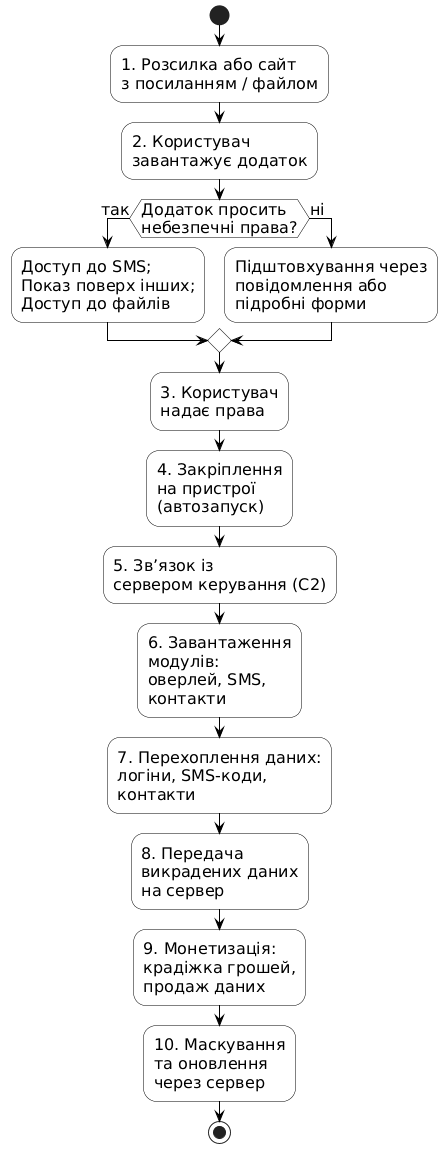
\includegraphics[width=0.45\linewidth]{img/figure6_6.png} 
    \caption{Сценарій небезпечних шахрайських схем}
    \label{fig:6_6}
\end{figure}

\newpage

Вищевказана схема показує спрощений сценарій атаки:

\begin{enumerate}
    \item \textbf{Доставка.} Шахрай розсилає покликання або підроблений додаток.
    \item \textbf{Інсталяція.} Користувач встановлює його і часто дає зайві права (дозволи).
    \item \textbf{Закріплення.} Програма закріплюється на пристрої, з'єднується з сервером шахрая (C2 server).
    \item \textbf{Виконання.} Підвантажує модулі для крадіжки даних і монетизації (гроші, файли, ботнет).
\end{enumerate}

Що стосується персональних комп'ютерів та серверів, спектр векторів атак є ширшим і включає складний фішинг, використання вразливостей операційних систем (експлойти) та Drive-by завантаження із заражених вебсайтів.

\subsection*{Приклад шахрайства: фейковий додаток (Львів)}

\textbf{Ситуація 1. Травень 2024 року}

Мешканець Львова, 42-річний приватний підприємець Андрій, о 10:12 отримав SMS-повідомлення з текстом: \textit{«Ваш рахунок заблоковано. Терміново підтвердьте доступ у застосунку»}.

\textbf{Соціальна інженерія.}
Відправником значився «MyBank Support», а в листі було покликання на сторінку з нібито офіційним мобільним додатком. Адреса виглядала переконливо — \texttt{https://mybannk-app.com/download}, де подвійна літера «n» була майже непомітною (тайпосквотинг). Переляк від можливої втрати доступу до рахунку після великого переказу змусив Андрія не звернути увагу на домен.

\newpage

\textbf{Технічна реалізація атаки.}
О 10:14 він завантажив установочний файл програми (файл із розширенням \texttt{.apk}\footnote{Формат файлу для встановлення додатків вручну на смартфон (ОС Android).}) і встановив додаток на свій Android-смартфон. Програма повністю імітувала офіційний банківський застосунок: логотип, кольори, меню входу.

Вже при запуску додаток попросив доступ до SMS та служби спеціальних можливостей (\textit{Accessibility Services}). Андрій погодився, не розуміючи ризиків.
Технічно це був банківський троян \textbf{«Xenomorph»}, який одразу почав:
\begin{itemize}
    \item перехоплювати одноразові коди з SMS;
    \item показувати фальшиві вікна для входу поверх справжнього застосунку банку (атака \textit{Overlay}).
\end{itemize}

\textbf{Фінансові та правові наслідки.}
О 10:19 з рахунку Андрія було здійснено три транзакції на загальну суму \textbf{147 000 грн}. Гроші спершу пішли на транзитний рахунок, а вже за кілька хвилин були переведені у криптовалюту.

\begin{itemize}
    \item \textbf{Економічно.} Андрій втратив місячний оборот бізнесу й був змушений оформити кредит для розрахунків із постачальниками. Банк відмовив у компенсації, оскільки клієнт самостійно встановив стороннє ПЗ.
    \item \textbf{Психологічно.} Він зазнав сильного стресу та почуття провини, вважаючи власну необережність причиною краху.
    \item \textbf{Юридично.} О 11:30 він подав заяву до кіберполіції; інцидент був кваліфікований за ст. 190 ККУ (шахрайство) та ст. 361 ККУ (несанкціоноване втручання в роботу комп’ютерних систем).
\end{itemize}

\newpage

\textit{\textbf{Висновки.} Цей випадок демонструє поєднання психологічного фактору (страх і терміновість) та технічної складової (фейковий .apk із правами Accessibility). Уникнути атаки можна було, якби Андрій завантажував застосунки лише з офіційного Google Play, перевірив адресу покликання та відмовився надавати критичні дозволи.}

\section{Додаткові приклади атак на смартфони}

Атаки на смартфони стали одними з найдинамічніших форм кіберзлочинності у 2024 році. За даними \textit{Google Threat Analysis Group}, понад \textbf{13 мільйонів} шкідливих застосунків було виявлено лише за один рік, а збитки користувачів від троянів, шпигунського ПЗ та програм-вимагачів на мобільних пристроях сягнули сотень мільйонів доларів.

\vspace{0.3cm}

\textbf{Типові сценарії прості:}
\begin{itemize}
    \item людина отримує SMS із покликанням на «оновлення банківського застосунку»;
    \item бачить рекламу у соцмережі з пропозицією завантажити «новий месенджер із функціями преміум»;
    \item знаходить «офіційний маркетплейс зі знижками».
\end{itemize}

Програма виглядає правдоподібно — знайомі кольори, логотипи, інтерфейс, але насправді містить троян чи шпигунський модуль. Після запуску вона запитує «звичайні» дозволи — доступ до SMS, геолокації, контактів чи мікрофона, і саме тут відбувається захоплення контролю.

\textit{Психологія працює на випередження:} поспіх («терміново підтвердьте доступ»), приваблива вигода («знижка 50\%»), або соціальний доказ («цей додаток уже завантажили тисячі»). Користувач під тиском не перевіряє адресу сторінки чи видавця у Play Store.

\subsection*{Історія 1. Як шахраї вкрали гроші: Історія Дмитра}

У вівторок, 19 листопада 2024 року, о 07:58 ранку мешканець Полтави Дмитро (31-річний інженер) отримав у Viber підозріле повідомлення. Воно було нібито від «підтримки банку “Обрій”» і вимагало «терміново перевірити пристрій», пропонуючи натиснути кнопку «Оновити додаток».

\textbf{Крок 1. Маскування під звичний інтерфейс}

покликання вело на сторінку, яка ідеально копіювала офіційний магазин Google Play, але адреса сайту була \texttt{obriy-app.com} — це була підробка, а не справжній сайт Google.

О 08:00 Дмитро натиснув «завантажити». Телефон запитав, чи дозволити браузеру (Chrome) встановлювати програми з невідомих джерел. Дмитро погодився і встановив шкідливий файл:
\begin{itemize}
    \item \textbf{Файл:} \texttt{ObriySecure\_v2.1.apk} (12,4 МБ)
    \item \textbf{Пакет:} \texttt{com.obriy.secure.update}
    \item \textbf{Хеш SHA-256:} \texttt{a91f...d4c7}
\end{itemize}

\textbf{Крок 2. Експлуатація фактору поспіху та довіри}

Під час першого запуску фейкова програма попросила надати їй кілька критично небезпечних дозволів. Програма запевнила, що все це потрібно «щоб активувати захист від шахрайства». Дмитро поспішав на ранкову нараду (о 9:00) і, під тиском терміновості, на все погодився:

\begin{enumerate}
    \item \textbf{«Служби доступності» (Accessibility Service).} Це найголовніший дозвіл. Він дозволяє програмі бачити абсолютно все на екрані та навіть натискати кнопки замість користувача.
    \item \textbf{«Доступ до сповіщень».} Щоб читати текст усіх сповіщень (включно з push-кодами від банку).
    \item \textbf{«Показ поверх інших програм».} Щоб створювати вікна-перехоплювачі (або імітовані інтерфейси) поверх оригінальних програм (Overlay attack).
    \item \textbf{«Доступ до SMS».} Щоб читати повідомлення з кодами підтвердження.
\end{enumerate}

\textbf{Як спрацювала атака (Технічний аспект)}

Технічно це був банківський вірус (троян). Хронологія злочину:

\begin{enumerate}
    \item \textbf{Крадіжка пароля (08:05).} Коли Дмитро відкрив справжній додаток банку, шкідлива програма помітила це і, використавши право накладати вікна поверх інших програм, миттєво показала ідеально скопійовану форму входу. Дмитро ввів у неї логін і пароль, і ці дані одразу відправилися на сервер зловмисників.
    
    \item \textbf{Перехоплення кодів (08:07).} Зловмисники ініціювали вхід в онлайн ‑ банкінг. Банк надіслав SMS‑код і повідомлення додатка для підтвердження, але троян, маючи доступ до сповіщень і SMS, автоматично перехопив ці коди і переслав їх на сервер зловмисників. Дмитро міг навіть не помітити цих повідомлень, оскільки троян може їх приховувати.
\end{enumerate}

\textit{Аналіз інциденту показав, що шкідливий додаток зареєстрував службу спеціальних можливостей, мав права читати SMS, отримувати повідомлення, накладати вікна поверх інших програм і автозапускатися при увімкненні телефону. У мережевих журналах зафіксовано регулярні звернення до сервера зловмисників і передачу зашифрованих даних.}

\subsection*{Фінал історії Дмитра: наслідки та результат}

О 08:09 та 08:11 з рахунку Дмитра вкрали \textbf{107 500 грн} (трьома переказами). Дмитро помітив серію сповіщень про списання грошей лише о 08:12. Він спробував зайти у свій банківський додаток, але бачив лише нескінченне завантаження («крутилку») — це вірус блокував йому доступ, продовжуючи показувати фальшивий екран. О 08:20 він додзвонився в банк і заблокував картку, а о 09:10 звернувся до кіберполіції.

\textbf{Результат.} Банк відмовив у компенсації. Юридична причина: Дмитро самостійно встановив програму не з офіційного магазину і надав їй критичні дозволи, що дозволило вірусу перехопити дані. Однак важливо розуміти: дії Дмитра не були проявом "наївності". Зловмисники використали стан стресу (ранкова нарада) та техніку оверлею, яка робить підміну інтерфейсу майже невидимою для людського ока. Це була професійна атака на психіку, а не просто технічна помилка чи необачність. До вечора Дмитро повністю скинув свій телефон до заводських налаштувань, змінив усі паролі та назавжди вимкнув у налаштуваннях можливість інсталяції з невідомих джерел, трансформувавши цей болючий досвід у навичку усвідомленої цифрової безпеки

\subsection*{Історія 2. «Віддалена заміна SIM-картки» (SIM-swapping): як втратити номер за 3 хвилини}

Механізм цієї атаки ілюструє реальна схема соціальної інженерії, яка активно використовується шахраями в месенджерах. Був звичайний вівторок, обідня перерва. Андрій, менеджер з логістики, гортав стрічку новин, коли у Viber надійшло повідомлення. Контакт мав ім’я «Мар’яна Vodafone», аватар — знайомий червоно-білий логотип оператора, а поруч із назвою був синій значок, що імітував позначку офіційного акаунта (рис.~\ref{fig:6_7-1s}).

Текст повідомлення був дивним і загрозливим:
\textit{«Скріншот надамо — подальші кроки для продовження. Змінювати SIM не потрібно, оскільки система формує серійний номер SIM-карти, яка встановлена у смартфоні. Лише після продовження необхідно виконати перезавантаження смартфону».}

\begin{figure}[H]
    \centering
    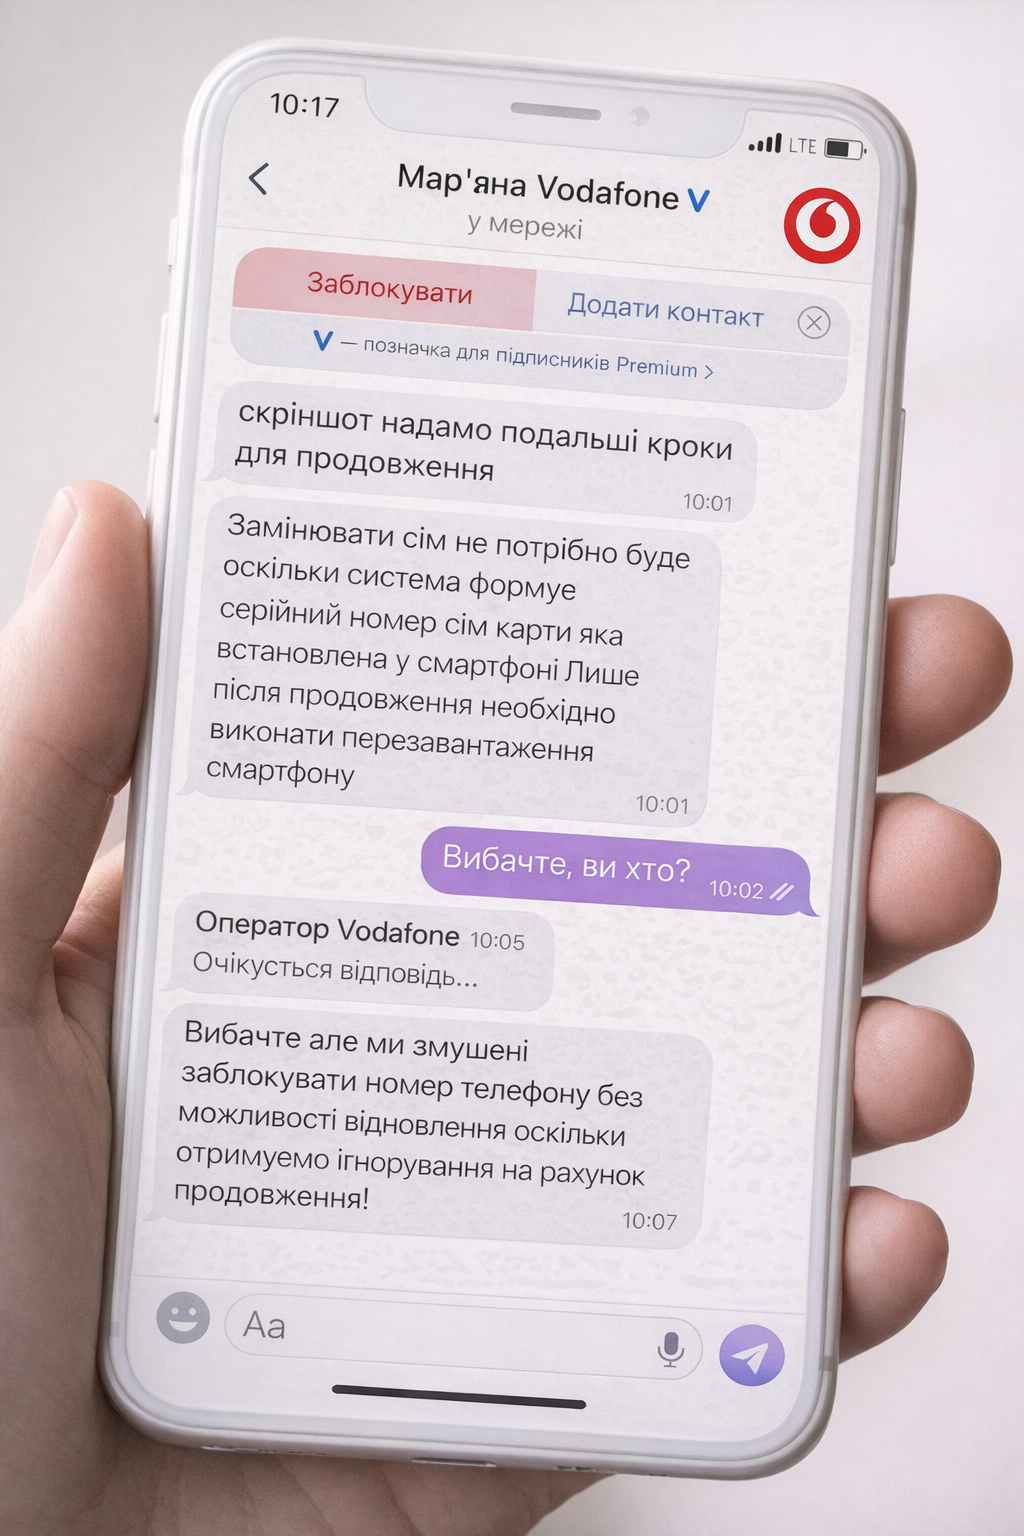
\includegraphics[width=0.75\linewidth]{img/fig6_7-1s.png}
    \caption{Приклад фейкового повідомлення від імені мобільного оператора у месенджері Viber}
    \label{fig:6_7-1s}
\end{figure}

Андрія насторожив тон повідомлення. Воно виглядало технічно й упевнено, але було плутаним. Він відповів коротко: \textit{«Вибачте, а ви хто?»}. 
Відповідь з’явилася майже одразу: \textit{«Оператор Vodafone»}.

Після цього співрозмовник написав: \textit{«Очікується відповідь»}, створюючи відчуття терміновості та контролю ситуації. Андрій не встиг нічого уточнити, як отримав нове повідомлення:

\textit{«Вибачте, але ми змушені заблокувати номер телефону без можливості відновлення, оскільки отримуємо ігнорування на рахунок продовження!»}

У цей момент Андрій відчув різкий страх. Цей номер був у нього 10 років: банки, пошта, робочі контакти, школа доньки — все було зав'язано на ньому. Втратити номер означало зупинити життя. Він швидко відповів: \textit{«Що мені робити? Я не можу їхати в салон, я на роботі».}

Відповідь прийшла миттєво: \textit{«Ми розуміємо. Для зручності клієнтів процедуру спрощено. Ми згенерували для вас віртуальний слот. Вам потрібно лише підтвердити перехід в офіційному додатку My Vodafone. Це безкоштовно».}

Це заспокоїло Андрія. Шахраї не просили номер картки, CVV-код чи пароль від Приват24. Вони навіть не скидали підозрілих посилань. Вони просили зайти в \textbf{офіційний} додаток оператора. Що може бути безпечніше?

\textit{«Зайдіть у меню "Послуги" $\rightarrow$ "Заміна SIM". Введіть серійний номер нової картки: 89380...»} — дбайливо інструктував «менеджер».

Андрій старанно виконав інструкції. Додаток запитав SMS-код для підтвердження заміни. 
— \textit{«Код прийшов. Вводити?»} — запитав Андрій у чаті.
— \textit{«Так, це фінальний крок для захисту номера».}

Він ввів код. На екрані з'явилося: «Заявку прийнято».

Через кілька хвилин зв’язок на телефоні зник. Індикатор мережі змінився на символ відсутності сигналу. «Мабуть, перезавантажується», — подумав Андрій і перезапустив пристрій. Але зв'язок не з'явився.

Вже через 5 хвилин Андрій спробував зайти в банківський застосунок Приват24 через Wi-Fi, щоб перевірити рахунок. Пароль не підходив. Доступ було втрачено. Він натиснув «Забули пароль?». При відновленні пароля система повідомила: \textit{«Код підтвердження надіслано на ваш номер»}. 

На номер, який вже працював в іншому телефоні під контролем зловмисників, за сотні кілометрів звідси. У цей момент Андрій усвідомив, що втратив не просто SIM-картку, а контроль над своєю цифровою ідентичністю.

\subsubsection*{Аналіз інциденту: чому схема спрацювала?}

Ця ситуація — класичний приклад соціальної інженерії, помноженої на довіру до офіційних інструментів.

\begin{enumerate}
    \item \textbf{Страх втрати.} Шахраї створили штучний дедлайн («номер буде заблоковано»), що відключило критичне мислення.
    \item \textbf{Ілюзія безпеки.} Жертву попросили скористатися офіційним додатком. Андрій думав, що якщо він у «рідній» програмі оператора, то йому нічого не загрожує. Він не знав, що функція «Заміна SIM» призначена для самостійної заміни картки на нову (яку ви купили в магазині), а не для «оновлення даних».
    \item \textbf{Підміна понять.} Вводячи серійний номер, який надіслали шахраї, Андрій фактично сказав системі: «Я купив нову SIM-картку (яка насправді вже була фізично у шахрая), перенесіть мій номер на неї».
\end{enumerate}

Злочинці використали техніку штучного прискореного зближення (rapid bonding), маскуючись під турботливу підтримку оператора. Використання офіційного додатка було лише способом знизити пильність. Це психологічна пастка: коли людина бачить знайомий логотип, її мозок автоматично переходить у режим довіри (валідація безпеки).

\subsection*{Інші сценарії атак}

\begin{description}
    \item[Історія 3. Фейковий банківський застосунок (Харків, 2024)]
    37‑річна вчителька Олена отримала SMS з покликанням на «оновлений додаток» банку. Встановила його (троян «Xenomorph»).
    \newline \textbf{Втрати:} 82 000 грн за 30 хвилин.
    \newline \textbf{Техніка.} Оверлей-атаки (фальшиві вікна поверх справжніх) + перехоплення SMS.

    \item[Історія 4. Фейковий маркетплейс (Київ, червень 2024)]
    29‑річний Максим встановив з Telegram «додаток знижок AliExpress» (.apk). Телефон почав показувати підроблені сторінки входу Google/Facebook.
    \newline \textbf{Втрати:} \$540 (викрадено дані карт з прив'язаних акаунтів).
    \newline \textbf{Техніка.} Фішинг-набір + MiTM-атака (перехоплення трафіку) + кейлогінг.

    \item[Історія 5. Фейковий месенджер (Одеса, вересень 2024)]
    18-річна Анна завантажила з сайту «YoWhatsApp» (мод месенджера). Додаток встановив троян \textit{Triada}, отримав root-права.
    \newline \textbf{Втрати:} 3 200 грн (приховані підписки на платні сервіси).
    \newline \textbf{Техніка.} Троян-завантажувач (Dropper), що діяв у фоновому режимі.

    \newpage

    \item[Історія 6. Фейковий криптогаманець (Дніпро, січень 2025)]
    34‑річний інвестор Ігор встановив з Google Play додаток-клона MetaMask. Після оновлення у ньому з’явився шкідливий код.
    \newline \textbf{Втрати:} 0,8 BTC (~1,3 млн грн) після введення seed-фрази.
    \newline \textbf{Техніка.} Атака на ланцюг поставок (\textit{supply-chain attack}) — чистий додаток стає шкідливим після апдейту.
\end{description}

\section*{Висновки}

Аналіз наведених випадків показує, що атаки через фейкові мобільні застосунки спираються на поєднання довіри користувачів до відомих брендів і технічних прийомів, які майстерно маскують справжню природу програми. Зловмисники копіюють логотипи, відтворюють інтерфейс і навіть іноді проходять початкову перевірку в офіційних магазинах, щоб створити ілюзію безпеки.

\textbf{Ключові фактори успіху атак:}
\begin{itemize}
    \item \textbf{Соціальна інженерія.} Користувачі надавали шкідливим програмам доступ, вважаючи це звичайною процедурою.
    \item \textbf{Технічна складність.} Використання оверлеїв, кейлогінгу та обходу двофакторної аутентифікації (2FA) через перехоплення SMS.
    \item \textbf{Безповоротність втрат.} Кошти швидко виводяться через транзитні рахунки та криптобіржі, що робить їх повернення майже неможливим.
\end{itemize}

Усі приклади доводять, що навіть ідеально схожий інтерфейс не гарантує безпеки. Лише поєднання уважності та базових навичок кібергігієни (завантаження тільки з офіційних сторів, перевірка дозволів) здатне зупинити атаку ще до введення даних.

\section{Ознаки зараження пристрою}

Якщо ви помітили ці ознаки, пам'ятайте: це не ваша вина. Сучасне шкідливе ПЗ розробляється так, щоб залишатися непомітним навіть для досвідчених користувачів. Ознаки зараження пристрою зазвичай проявляються поступово, але їх можна помітити, якщо уважно стежити за поведінкою смартфона чи комп’ютера.

Практичний аспект кібергігієни передбачає використання спеціалізованих інструментів для аналізу підозрілих файлів. Покрокові методи перевірки безпеки програм та інтерфейси відповідних сервісів детально проілюстровано на рис.~\ref{fig:6_7}--\ref{fig:6_16}.

\begin{figure}[H]
    \centering
    
\includegraphics[width=0.60\linewidth]{img/figure6_7.jpg} 
    \caption{Порівняння фейкового та справжнього сайту}
    \label{fig:6_7}
\end{figure}

\begin{figure}[H]
    \centering
    
\includegraphics[width=0.80\linewidth]{img/figure6_8.jpg} 
    \caption{Порівняння фейкового та справжнього сайту}
    \label{fig:6_8}
\end{figure}

\begin{figure}[H]
    \centering
    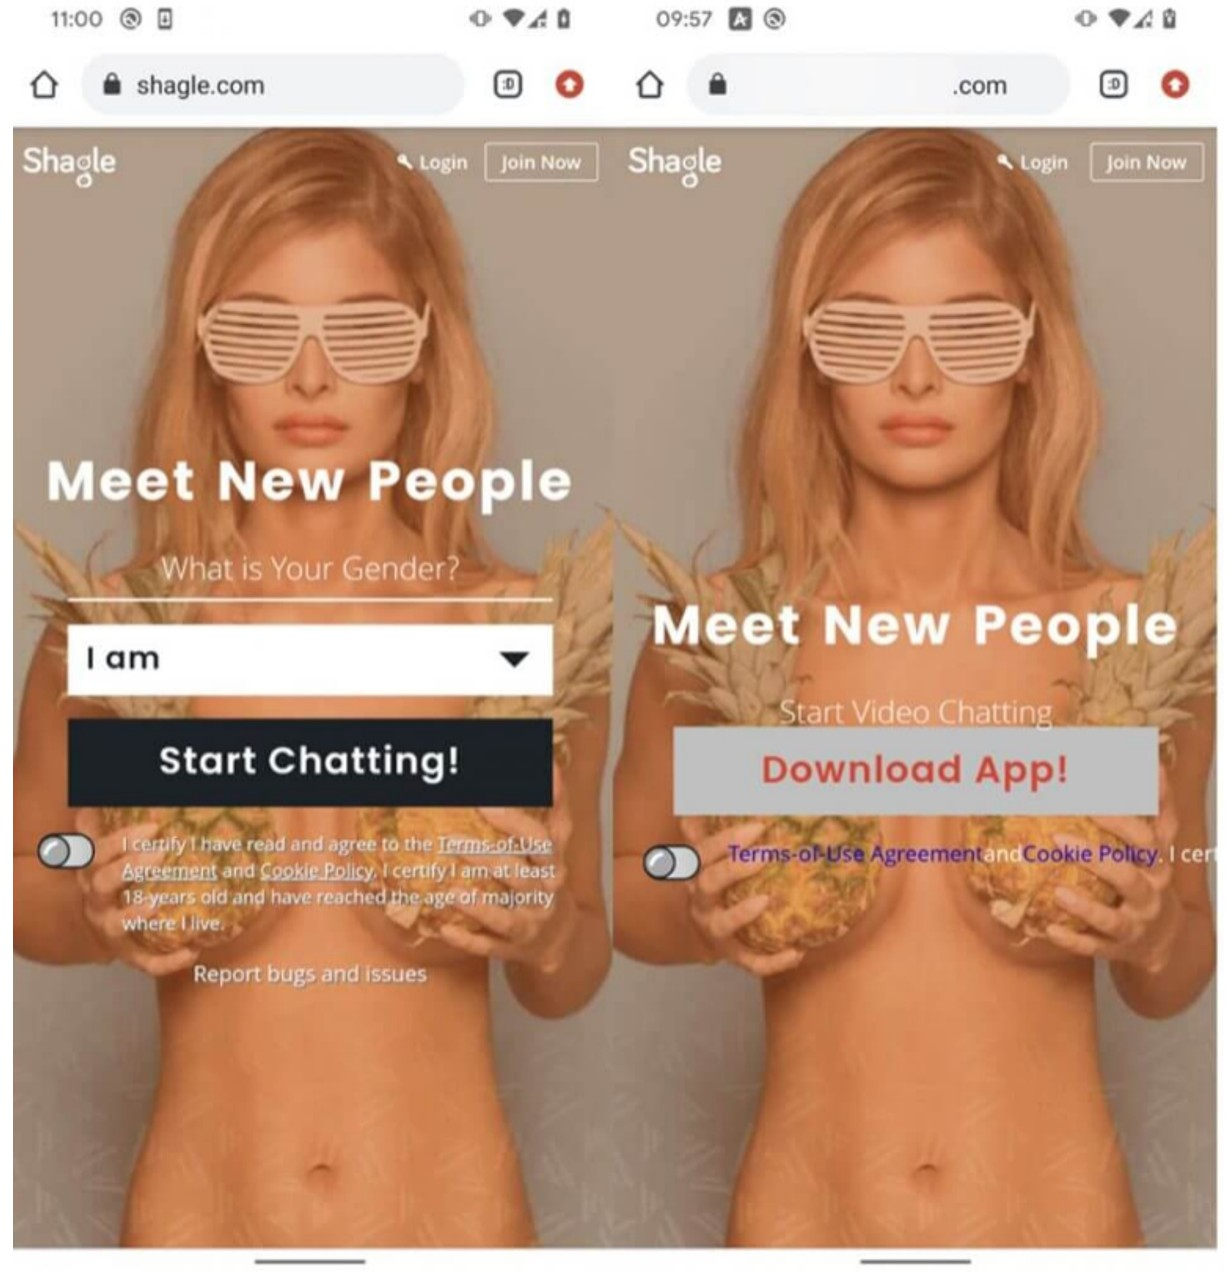
\includegraphics[width=0.90\linewidth]{img/figure6_9.jpg} 
    \caption{Аналіз справжніх додатків в GoogleStore}
    \label{fig:6_9}
\end{figure}

\begin{figure}[H]
    \centering
    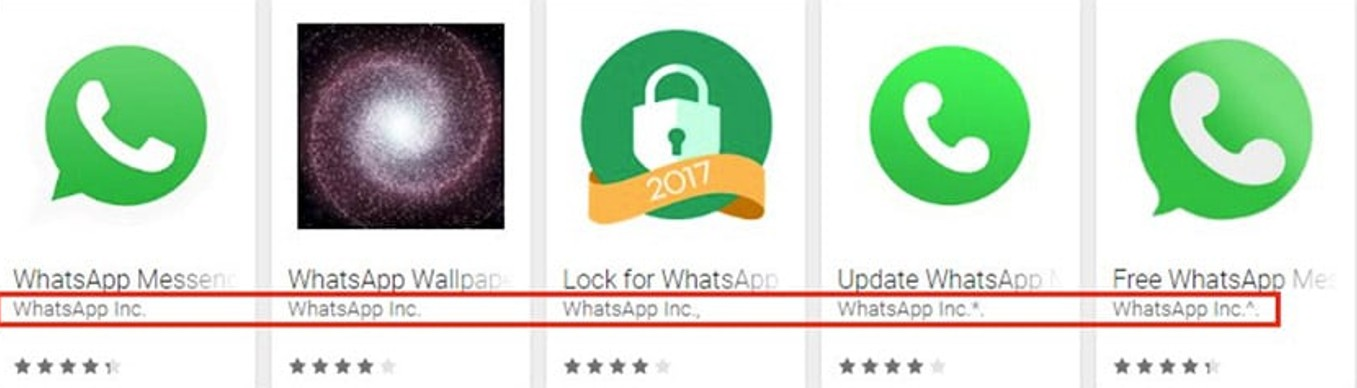
\includegraphics[width=0.90\linewidth]{img/figure6_10.jpg} 
    \caption{Порівняння фейкового та справжнього сайту}
    \label{fig:6_10}
\end{figure}

\begin{figure}[H]
    \centering
    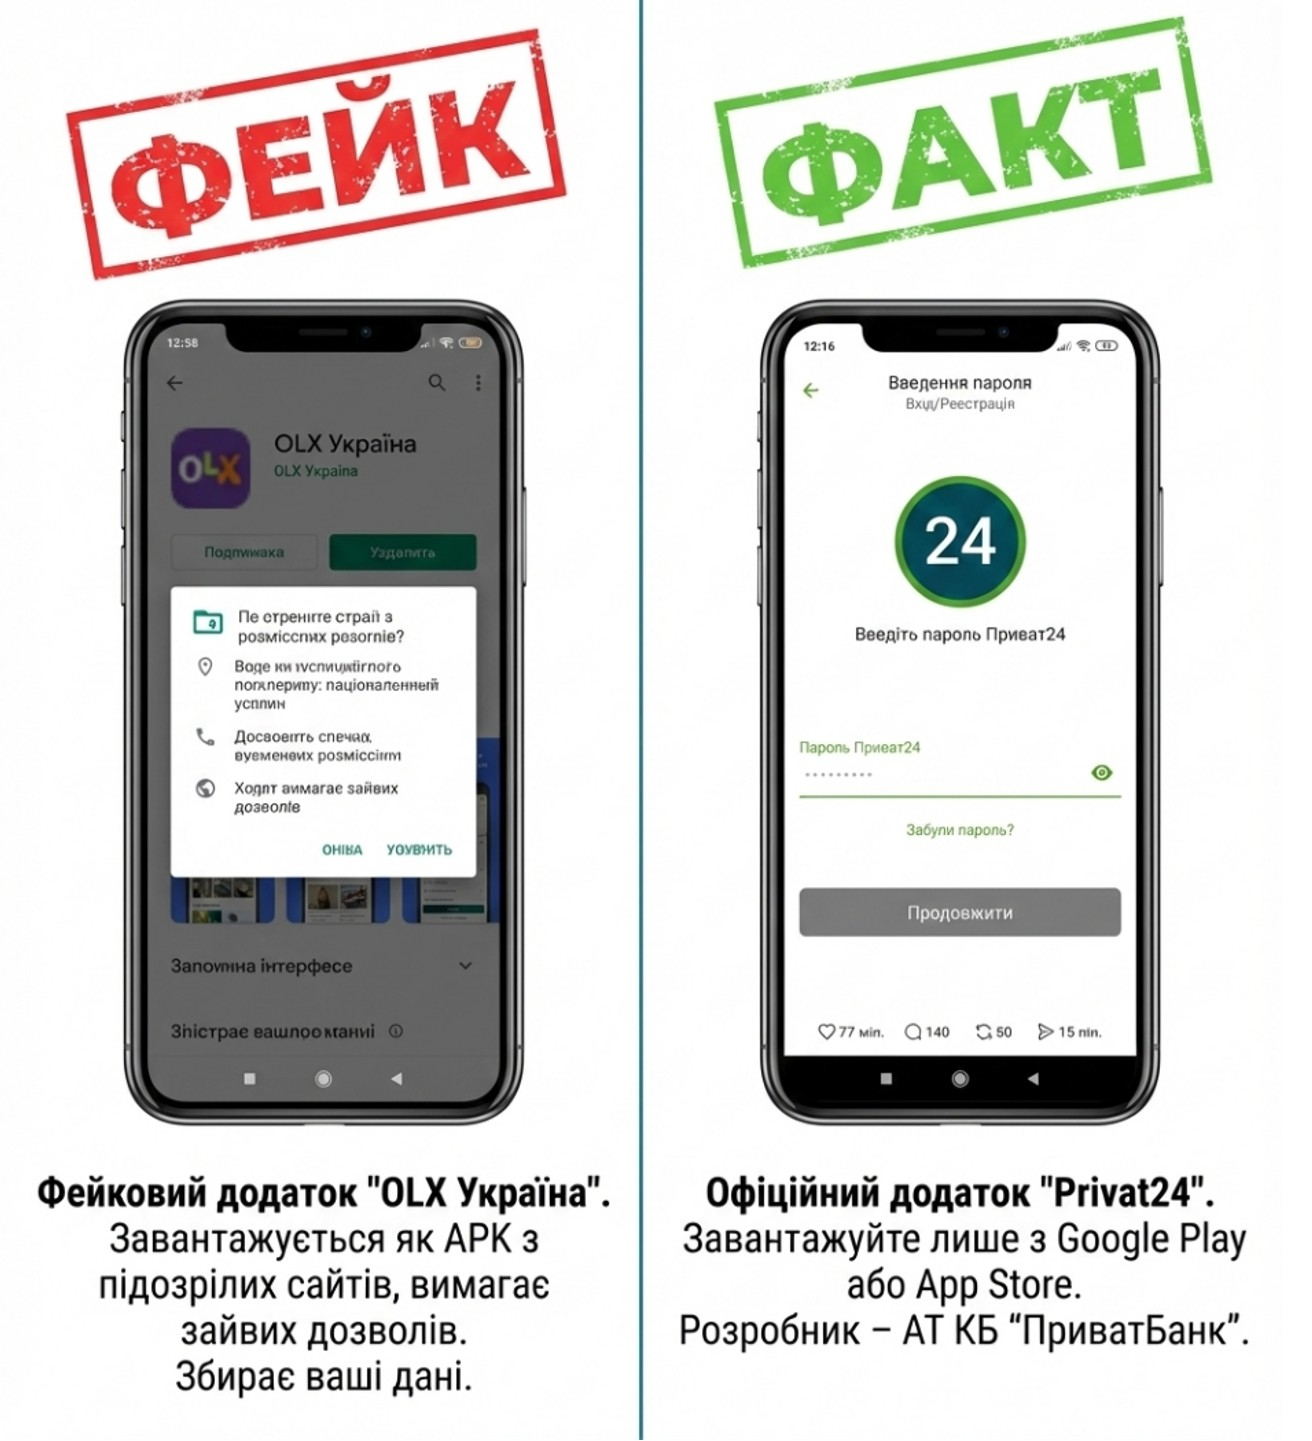
\includegraphics[width=0.60\linewidth]{img/figure6_11.jpg} 
    \caption{Порівняння фейкового та справжнього додатку}
    \label{fig:6_11}
\end{figure}

\begin{figure}[H]
    \centering
    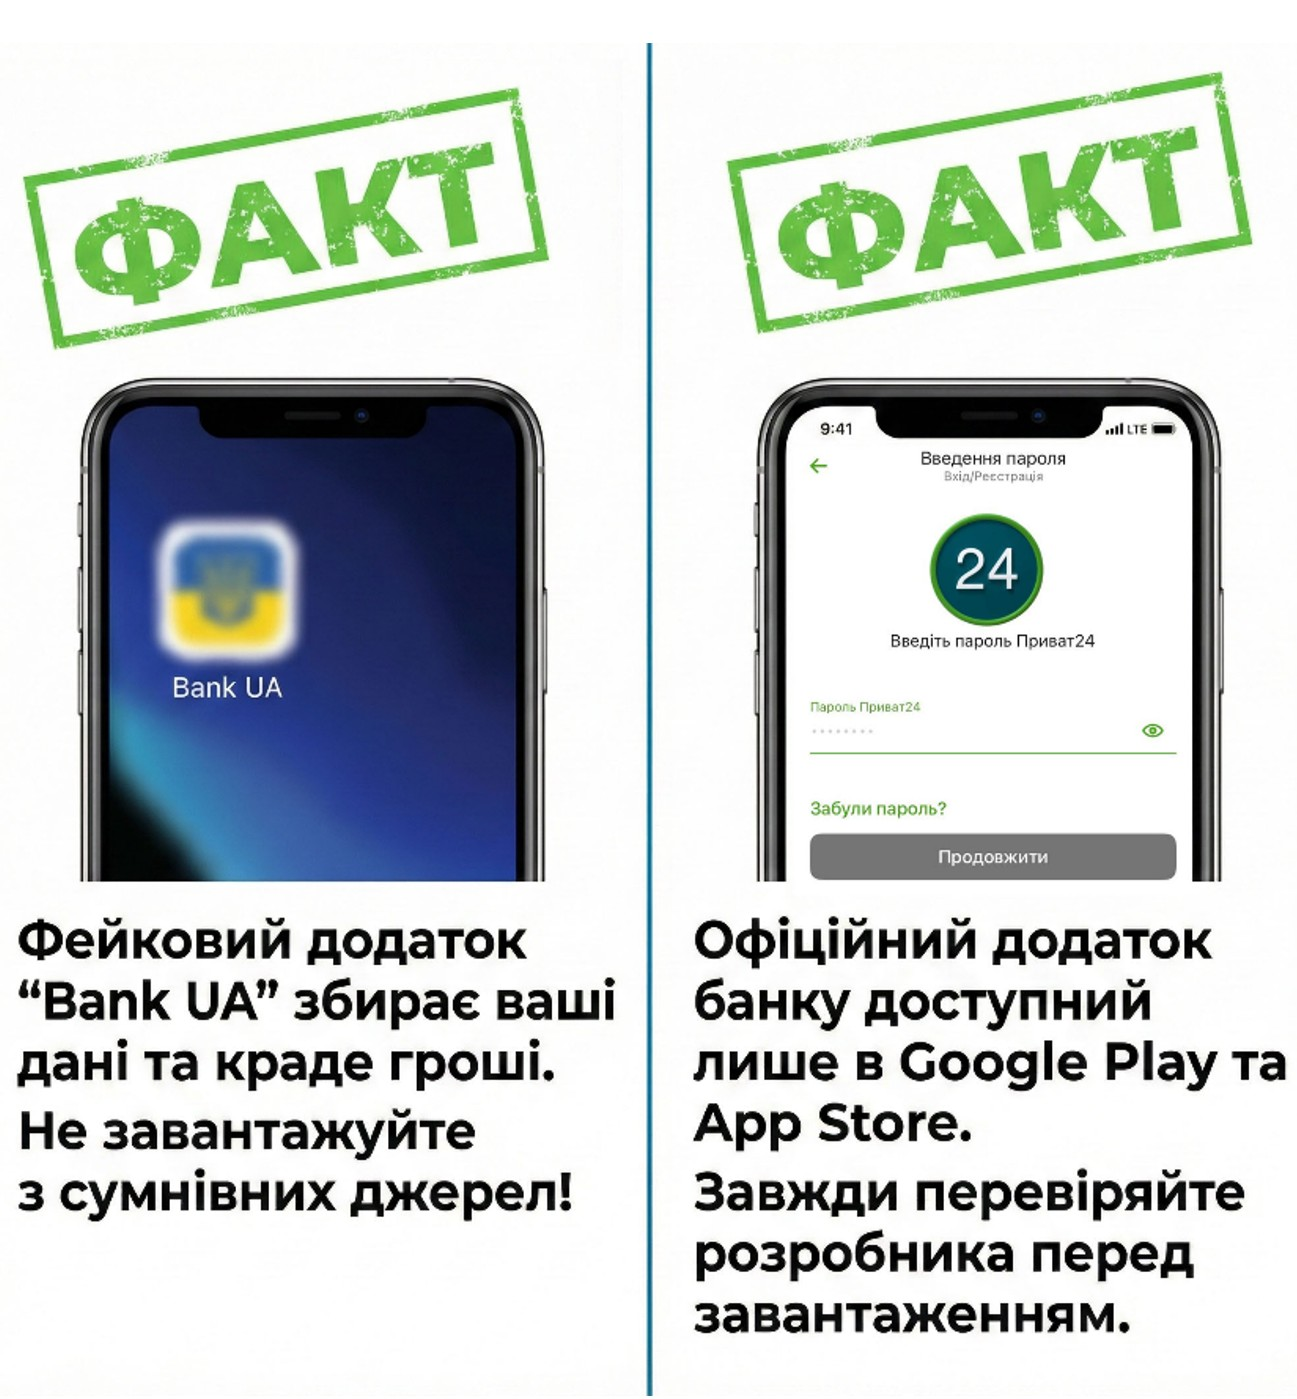
\includegraphics[width=0.60\linewidth]{img/figure6_12.jpg} 
    \caption{Листування щодо скачування фейкового додатку}
    \label{fig:6_12}
\end{figure}

\begin{figure}[H]
    \centering
    
\includegraphics[width=0.70\linewidth]{img/figure6_13.jpg} 
    \caption{Листування з другом щодо скачування фейкового додатку}
    \label{fig:6_13}
\end{figure}

\begin{figure}[H]
    \centering
    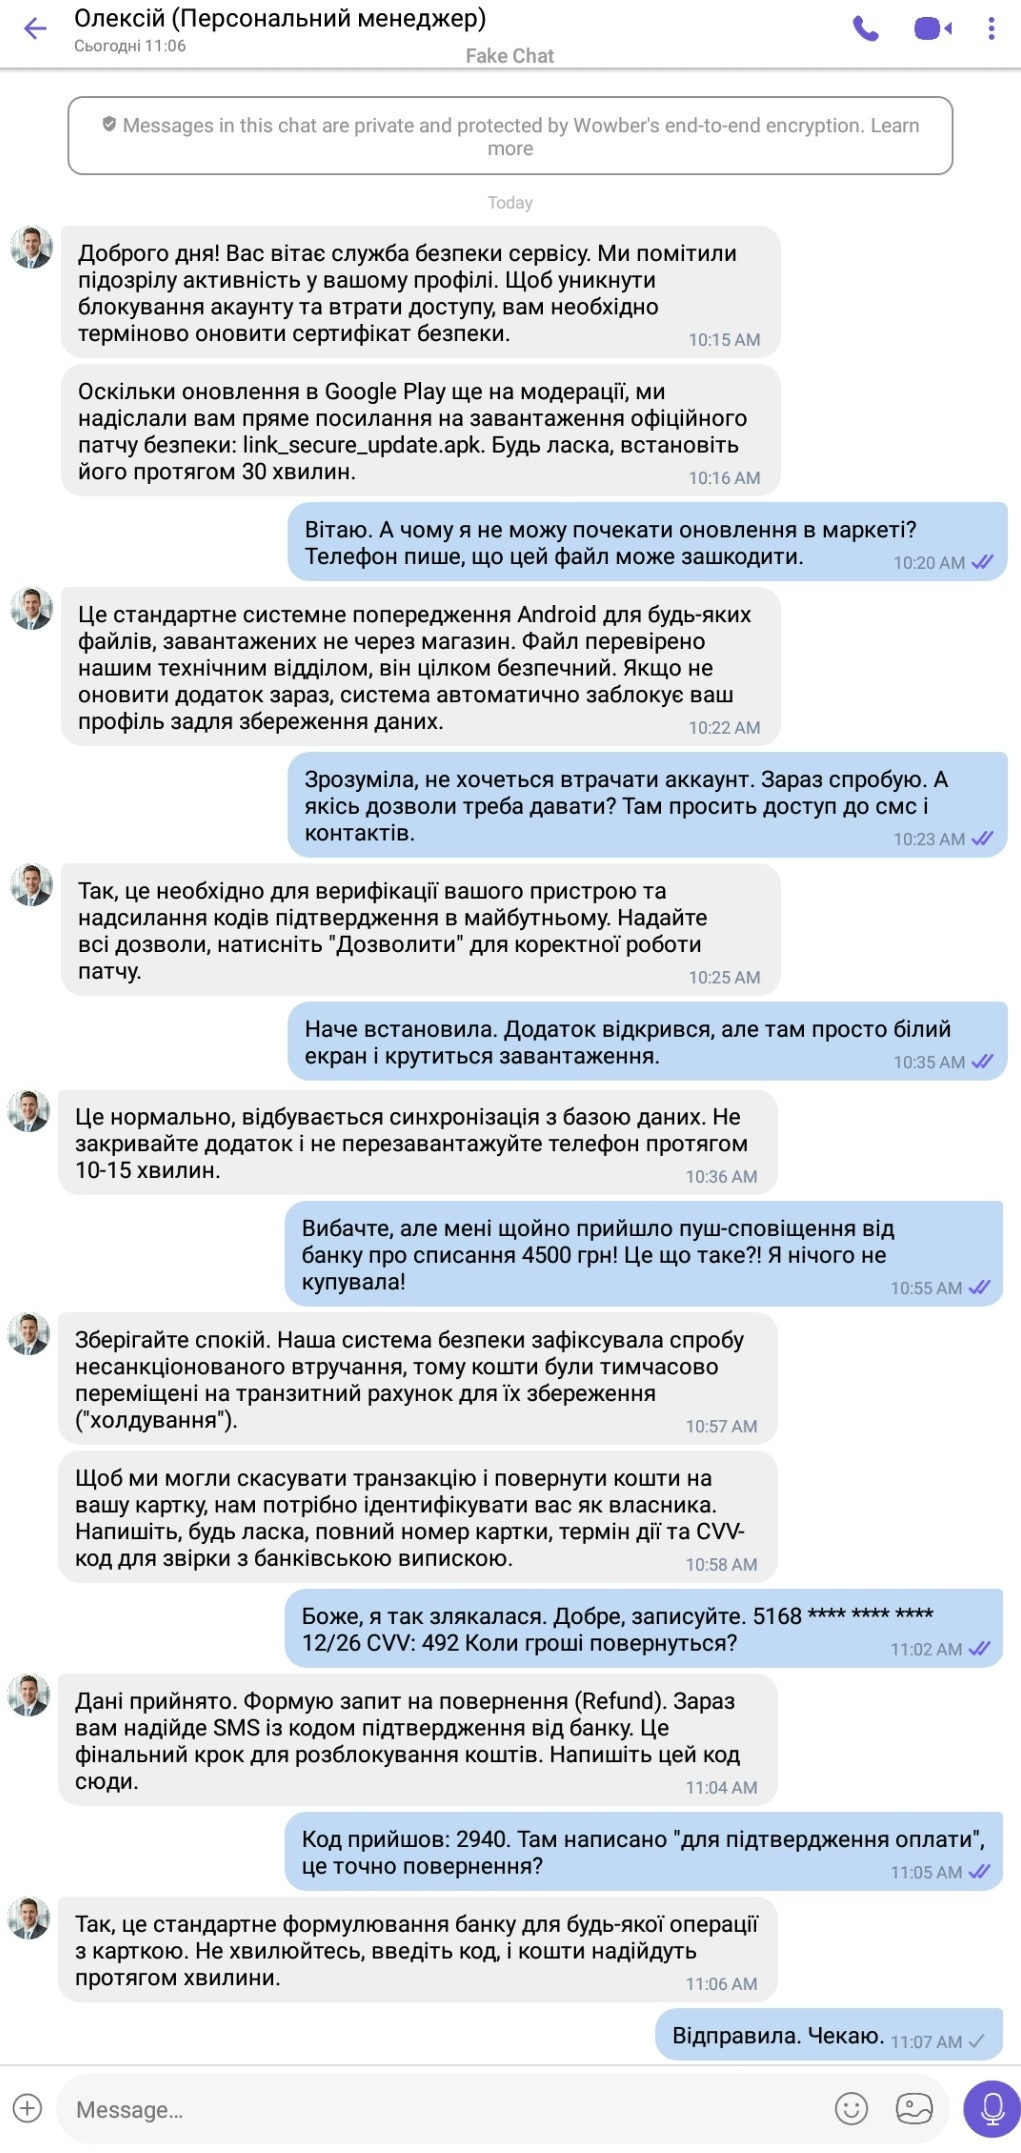
\includegraphics[width=0.70\linewidth]{img/figure6_14.jpg} 
    \caption{Листування щодо скачування фейкового додатку}
    \label{fig:6_14}
\end{figure}

\begin{figure}[H]
    \centering
    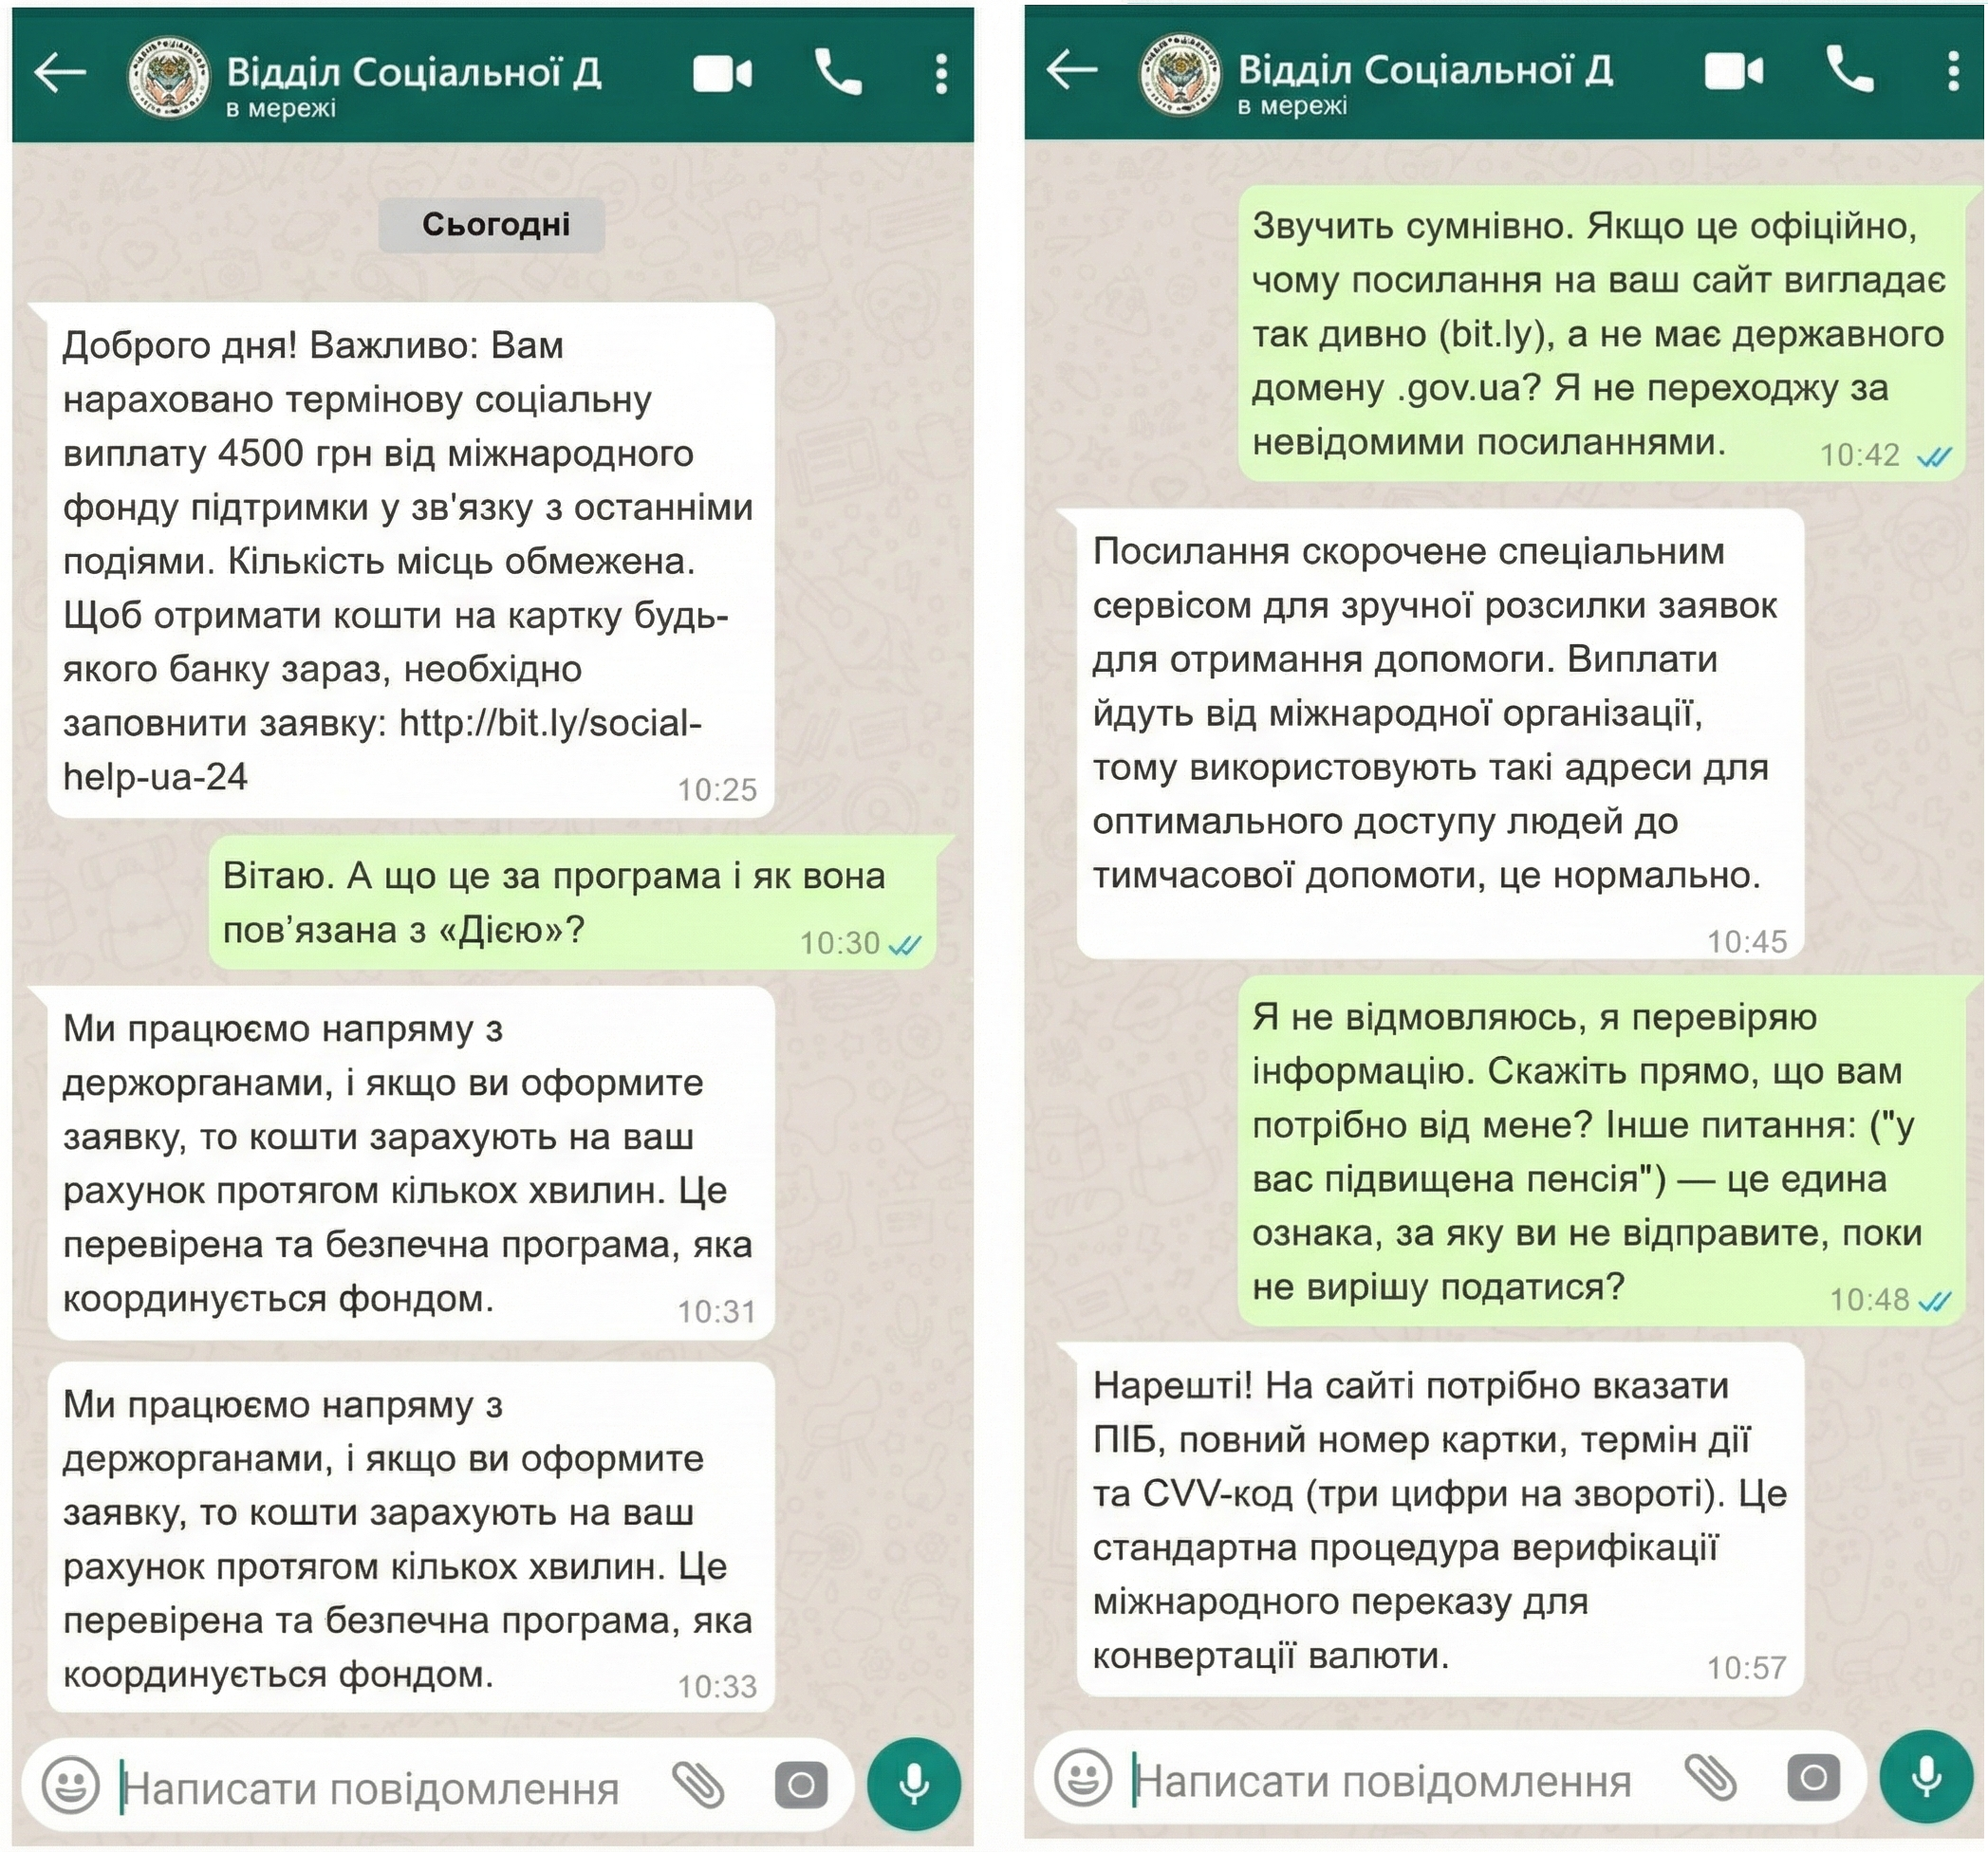
\includegraphics[width=0.75\linewidth]{img/figure6_15.png} 
    \caption{Листування щодо скачування фейкового додатку}
    \label{fig:6_15}
\end{figure}

\begin{figure}[H]
    \centering
    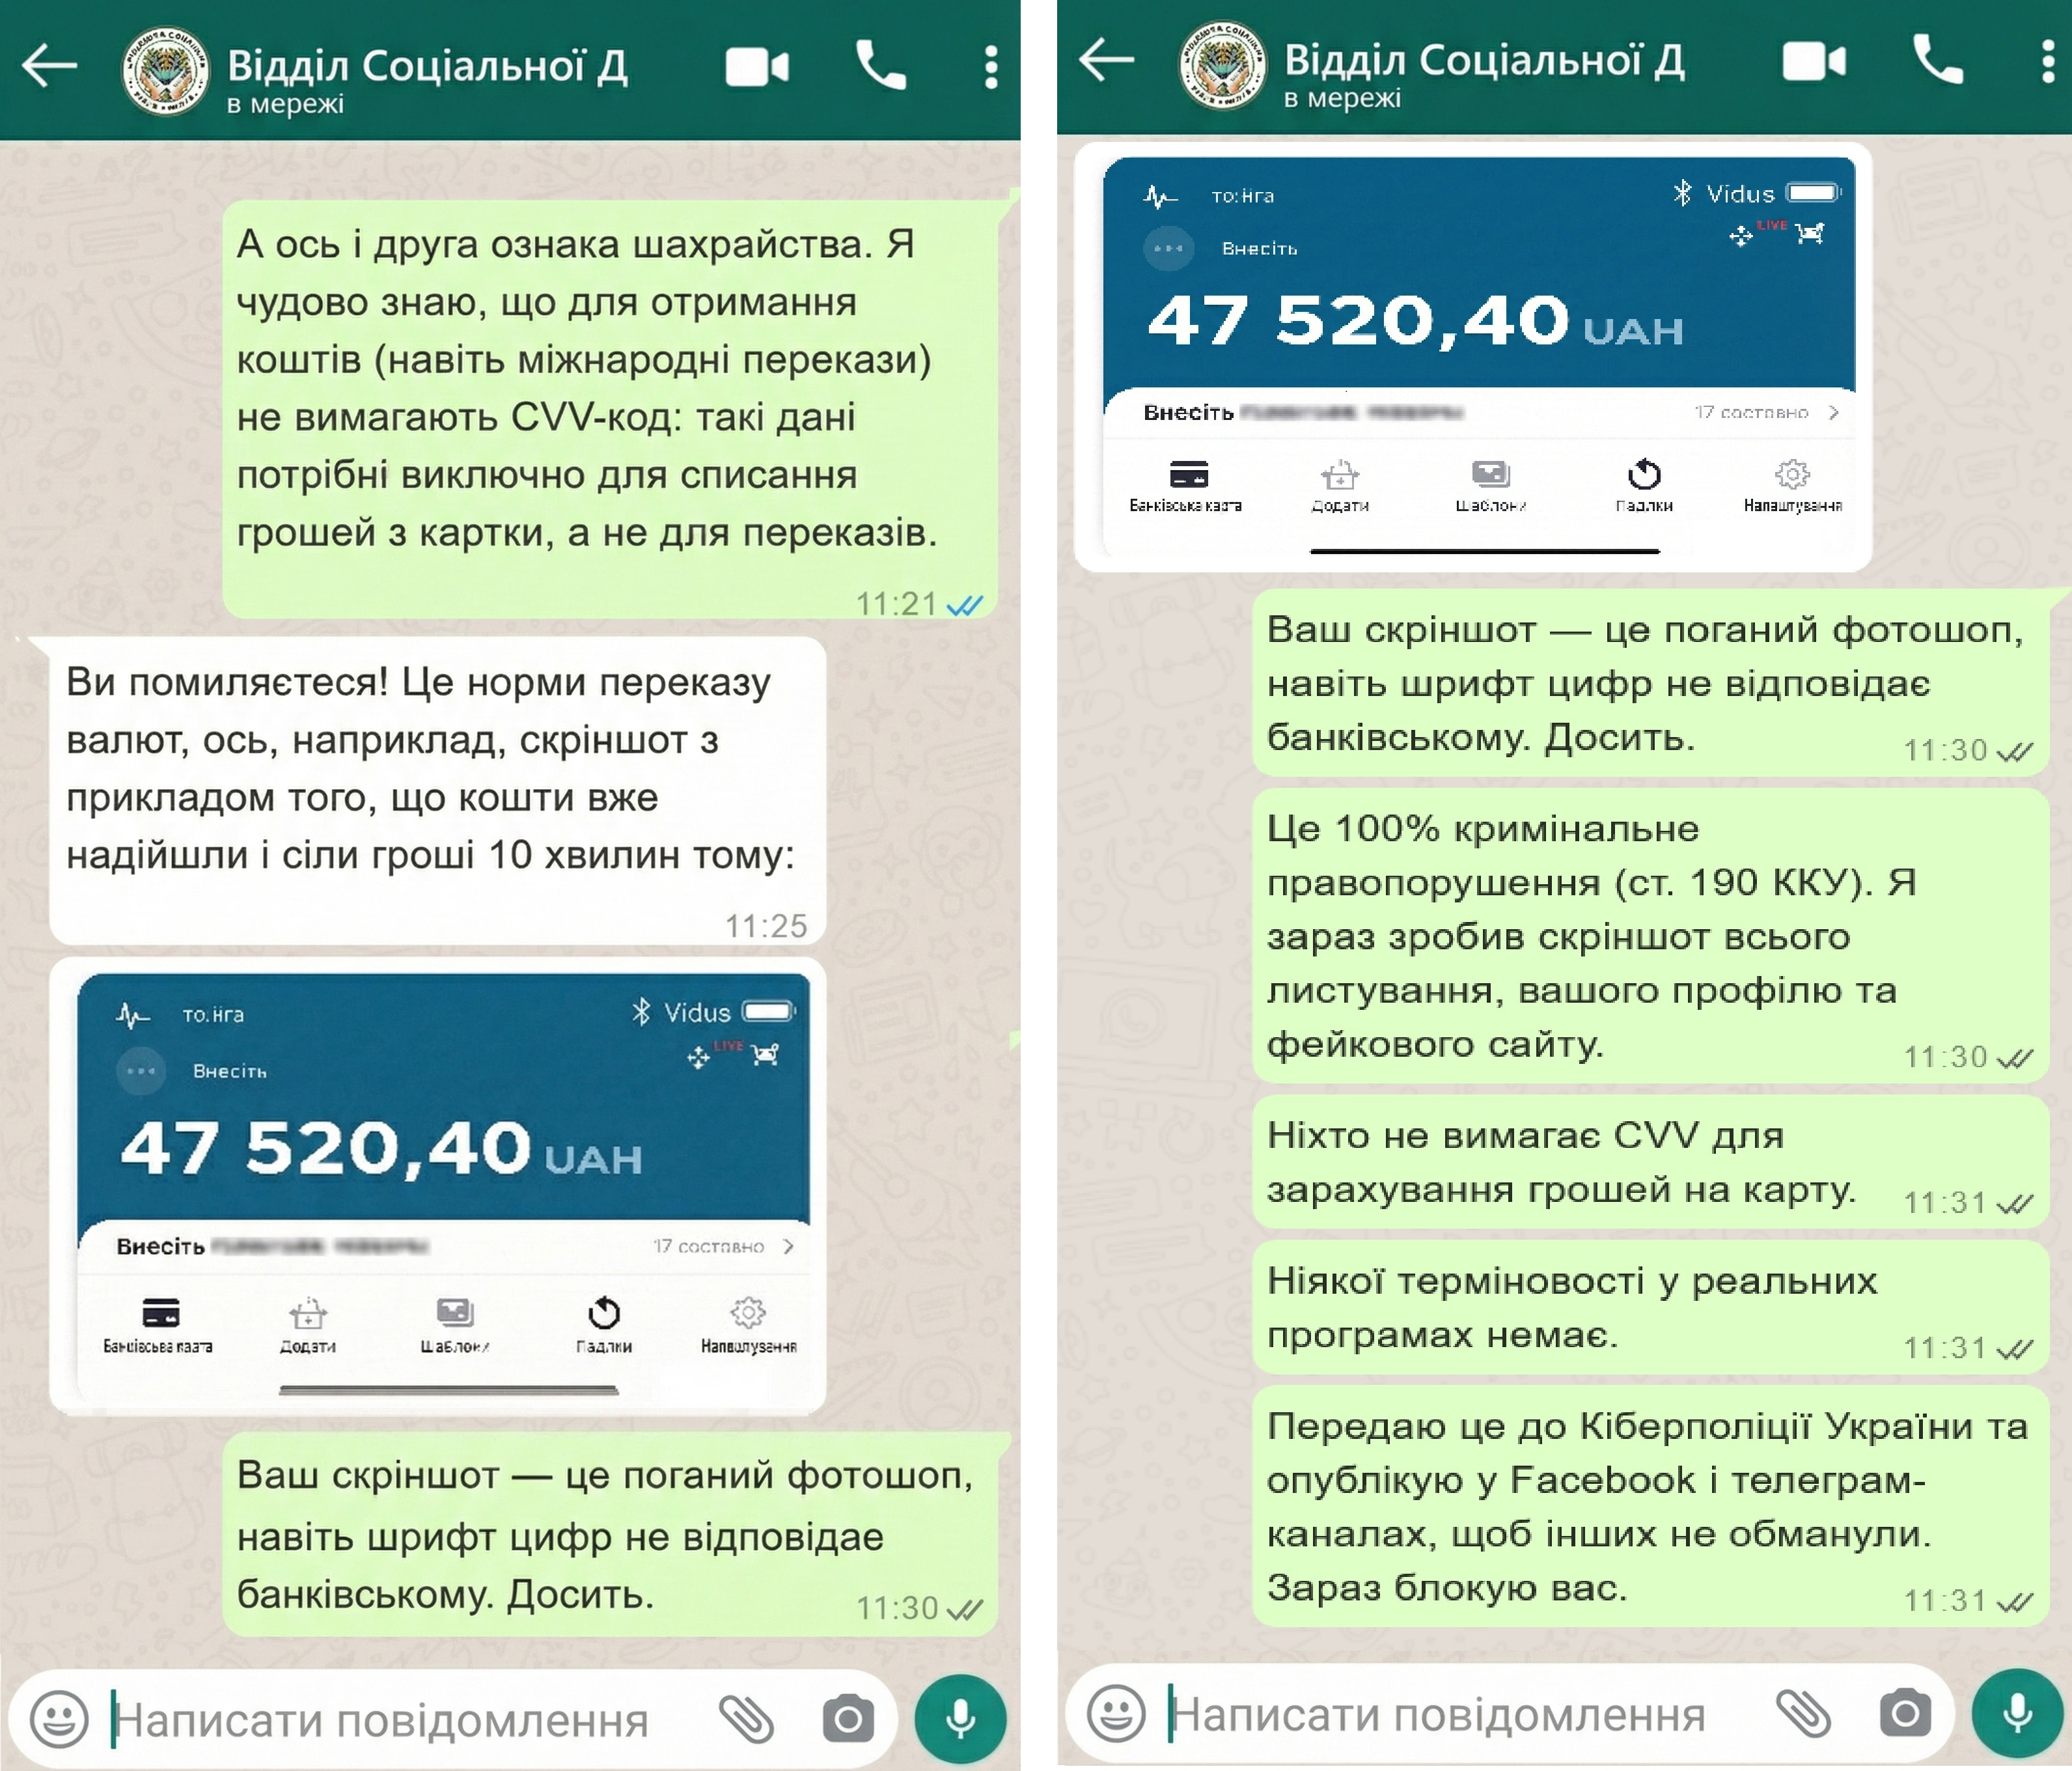
\includegraphics[width=0.75\linewidth]{img/figure6_16.jpg} 
    \caption{Листування з шахраєм}
    \label{fig:6_16}
\end{figure}

Як зрозуміти, що ваш смартфон під загрозою? Існує низка технічних та поведінкових індикаторів:

\begin{itemize}
    \item \textbf{Повільна робота, швидка розрядка та перегрів.}
    Наприклад, смартфон «гальмує» без причини, а батарея сідає набагато швидше, ніж зазвичай. Технічно це означає, що шкідливе ПЗ працює у фоні, постійно навантажуючи процесор або графічний чіп (наприклад, для прихованого майнінгу криптовалют чи участі в DDoS-атаках).

    \item \textbf{Поява незрозумілих додатків та іконок.}
    Наприклад, на робочому столі з’являються програми, які ви точно не встановлювали. Це пряма ознака того, що троян-завантажувач вже отримав контроль над системою і самостійно інсталює нові шкідливі модулі.

    \item \textbf{Несподівані зміни в налаштуваннях.}
    Наприклад, самовільно змінилася стартова сторінка в браузері, з'явилися невідомі розширення або додатки раптом отримали небезпечні дозволи (наприклад, доступ до «Спеціальних можливостей»), хоча ви їх не надавали.

    \item \textbf{Нав'язлива реклама та перенаправлення.}
    Наприклад, рекламні вікна з’являються хаотично, навіть поверх інших програм чи екрану блокування. Браузер може автоматично переходити на невідомі сайти. Це класична робота \textit{Adware} (рекламного ПЗ).

    \item \textbf{Аномалії з банківськими додатками та фінансами.}
    Наприклад, ви помічаєте SMS про дрібні списання чи транзакції, які ви не робили. Або ж справжній банківський додаток раптом блокується, і з'являється фальшиве вікно з вимогою повторно ввести пароль чи PIN-код («оверлей-атака»).

    \newpage

    \item \textbf{Скарги від друзів на спам.}
    Наприклад, ваші контакти у месенджерах чи пошті починають отримувати від вас дивні повідомлення з покликаннями. Це означає, що хробак чи троян вже використовує ваш акаунт та пристрій для подальшого поширення інфекції.

    \item \textbf{Підозріла активність камери, мікрофона та мережі.}
    Наприклад, індикатор камери чи мікрофона вмикається сам по собі, коли ви не використовуєте додатки. Також може фіксуватися аномально велике використання мобільних даних у фоновому режимі — це пристрій зв'язується з серверами зловмисників.
\end{itemize}

\textit{Якщо ви помітили одну або декілька з цих ознак, це вагомий привід негайно перевірити систему. Не ігноруйте ці сигнали, оскільки вони рідко виникають без причини.}

\subsection*{Як діяти в таких ситуаціях?}

\begin{enumerate}
    \item \textbf{Негайно відключіть пристрій від Інтернету} (Wi-Fi та мобільні дані), щоб зупинити передачу даних зловмисникам.
    \item \textbf{Перевірте останні встановлені додатки} та видаліть усе підозріле, що ви не встановлювали особисто.
    \item \textbf{Запустіть повне сканування} надійним мобільним антивірусом.
    \item \textbf{Перевірте дозволи} (особливо «Спеціальні можливості» та «Адміністратори пристрою») і відкличте їх у сумнівних програм.
    \item \textbf{Крайній захід.} Якщо нічого не допомагає — зробіть резервну копію важливих даних (лише фото, документи) та виконайте повне скидання до заводських налаштувань.
\end{enumerate}


\section{Методи перевірки безпеки програм}

Не встановлюйте програму одразу, особливо якщо вона отримана поза офіційним магазином. Будь-який застосунок (файл \texttt{.apk}, \texttt{.exe}) чи покликання з месенджера або пошти вимагає перевірки ще до запуску.

\textit{Алгоритм екстреної дії.} Якщо ви вже встановили щось підозріле, негайно відключіть пристрій від Інтернету (Wi-Fi, мобільні дані), щоб зупинити зв'язок із серверами зловмисників. Перезавантажте пристрій у «Безпечному режимі» (Safe Mode), перевірте список дозволів та видаліть програму.

Далі — три рівні перевірки за допомогою доступних ресурсів. Якщо бодай один пункт викликає сумнів — не встановлюйте програму.

\subsection*{1. Перевірка джерела та репутації (Хто автор?)}

\begin{itemize}
    \item \textbf{1.1. Офіційні магазини.} Встановлюйте програми переважно з офіційних джерел. Перевіряйте ім’я розробника, відгуки та кількість завантажень:
    \begin{itemize}
        \item Google Play: \url{https://play.google.com}
        \item Apple App Store: \url{https://apps.apple.com}
        \item Microsoft Store: \url{https://apps.microsoft.com/}
    \end{itemize}

    \item \textbf{1.2. Перевірка покликання (URL).} Перш ніж завантажувати файл, перевірте адресу:
    \begin{itemize}
        \item \textbf{VirusTotal} (перевіряє десятками антивірусів): \url{https://www.virustotal.com/}
        \item \textbf{URLScan} (показує, куди перенаправляється запит): \url{https://urlscan.io/}
        \item \textbf{PhishTank} (база фішингових сайтів): \url{https://www.phishtank.com}
    \end{itemize}

    \item \textbf{1.3. Перевірка домену.} Перевірте вік сайту. Шахрайські ресурси часто зареєстровані лише кілька днів тому:
    \begin{itemize}
        \item ICANN Lookup: \url{https://lookup.icann.org/}
        \item Whois: \url{https://www.whois.com/whois}
    \end{itemize}

    \item \textbf{1.4. Бази шахраїв.} Перевірка підозрілих сайтів, телефонів, карток:
    \begin{itemize}
        \item Сервіс Асоціації ЄМА: \url{https://www.stopfraud.com.ua}
        \item Кіберполіція: \url{https://ticket.cyberpolice.gov.ua}
        \item Перевірка посилань: \url{https://checkmylink.net/}
    \end{itemize}
\end{itemize}

\subsection*{2. Технічний аналіз файлу (До запуску)}

Якщо ви вже завантажили файл, але ще не запустили його:

\begin{itemize}
    \item \textbf{2.1. Статичний аналіз.} Завантажте файл на сервіс для сканування:
    \begin{itemize}
        \item VirusTotal (вкладка File): \url{https://www.virustotal.com/}
        \item Kaspersky OpenTip: \url{https://opentip.kaspersky.com/}
    \end{itemize}

    \item \textbf{2.2. Аналіз у пісочниці (Sandbox).} Спостереження за запуском у безпечному середовищі:
    \begin{itemize}
        \item ANY.RUN (інтерактивний аналіз): \url{https://any.run}
        \item Hybrid Analysis (Falcon Sandbox): \url{https://www.hybrid-analysis.com}
    \end{itemize}
    
    \item \textbf{2.3. Перевірка цифрового підпису.} Переконайтеся, що файл підписаний оригінальним розробником (використовуйте інструменти \texttt{apksigner} для Android або \texttt{codesign} для macOS).
\end{itemize}

\subsection*{3. Аналіз поведінки (Після встановлення)}

\begin{itemize}
    \item \textbf{3.1. Антивірусне сканування.}
    Використовуйте \textbf{Google Play Protect} (Android), \textbf{Windows Defender} (Windows) або сканери за вимогою (\textbf{Malwarebytes}, \textbf{ESET Online Scanner}).
    
    \item \textbf{3.2. Моніторинг активності.}
    Використовуйте інструменти на кшталт \textbf{TCPView} (для відстеження мережевих з'єднань) або \textbf{Process Explorer} (для виявлення прихованих процесів) із пакету Microsoft Sysinternals.
\end{itemize}

\section*{Висновки та рекомендації}

\textbf{Короткі правила безпеки:}
\begin{enumerate}
    \item Спершу перевірка на VirusTotal, потім — завантаження.
    \item Завантажуйте лише з офіційних магазинів.
    \item Сумнівні дозволи — ознака шахрайства (наприклад, «Ліхтарик» просить доступ до SMS).
    \item Не надавайте дозвіл на «Спеціальні можливості» (Accessibility) без абсолютної впевненості.
\end{enumerate}

\textbf{Важлива рекомендація.}
У контексті захисту від мобільного шахрайства критично важливою є перевірка джерела завантаження. Асоціація ЄМА наполегливо рекомендує перед переходом за покликаннями для завантаження файлів (особливо з невідомих джерел) здійснювати верифікацію URL-адреси через спеціалізований сервіс \textbf{CheckMyLink} (\url{https://check.ema.com.ua/}).

\newpage

Актуальність цього інструменту зумовлена поширенням банківських троянів, які маскуються під корисні утиліти або ігри. Використання сканера дозволяє виявити загрозу ще на етапі переходу за покликанням, попередивши завантаження шкідливого контенту та компрометацію платіжних даних користувача~\cite{EMA_CheckMyLink}.

Узагальнений підхід до верифікації програмного забезпечення, що поєднує автоматизований аналіз та ручну перевірку, представлено на рис.~\ref{fig:6_17}.

\begin{figure}[H]
    \centering
    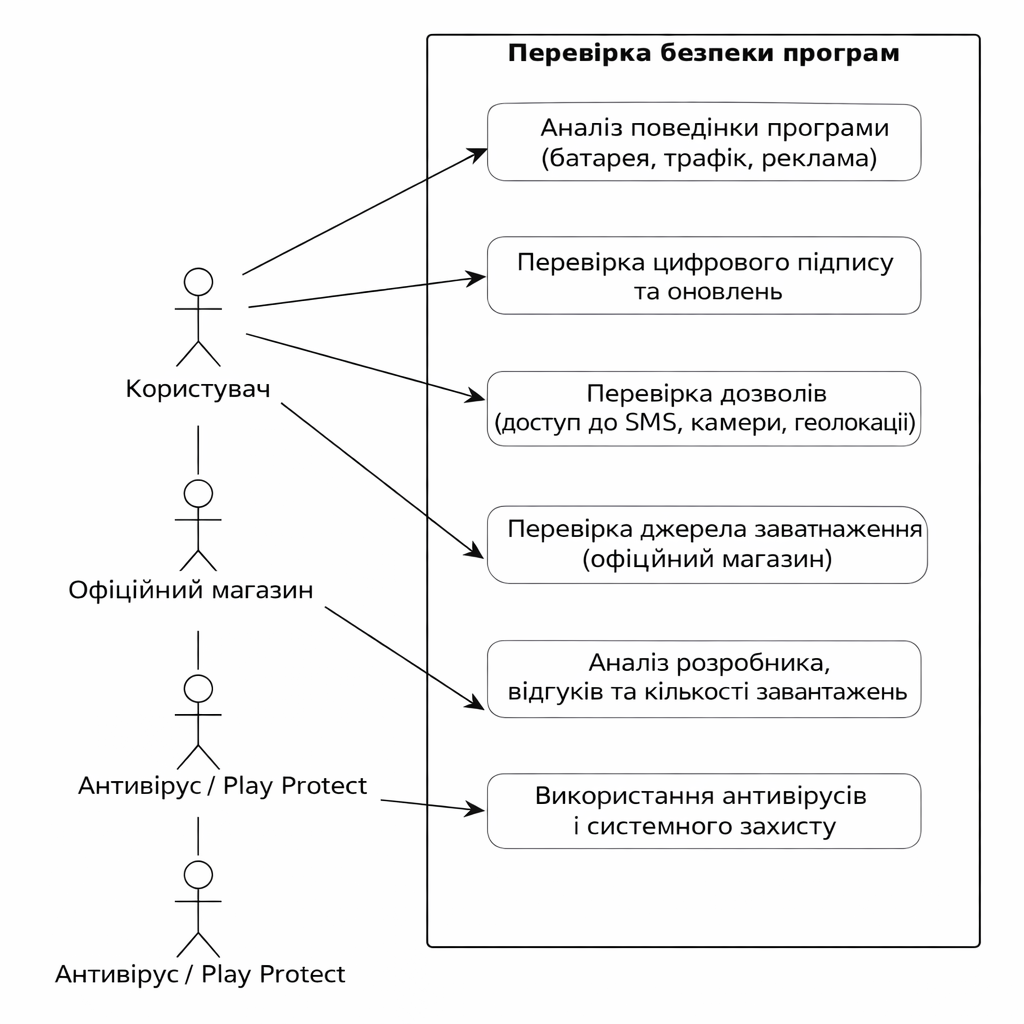
\includegraphics[width=0.95\linewidth]{img/figure6_17.png} 
    \caption{Методи перевірки безпеки програм}
    \label{fig:6_17}
\end{figure}

\section{Поради щодо безпечного завантаження програм}

Безпечне завантаження програм — це поєднання уважності, критичного мислення й дотримання простих правил цифрової гігієни. Дотримуючись їх, ви зменшите ризик інфікувати пристрій і запобігти більшості атак.

\begin{enumerate}
    \item \textbf{Завантажуйте тільки з офіційних магазинів.}
    Використовуйте Google Play, App Store або Microsoft Store. Ці магазини мають вбудовані механізми перевірки додатків (наприклад, Play Protect). Файли з розширенням \texttt{.apk} чи \texttt{.exe} зі сторонніх сайтів, форумів чи покликання з месенджерів несуть найвищий ризик зараження.

    \item \textbf{Користуйтеся захистом.}
    Встановіть надійний антивірус або захисний додаток (відомі продукти від ESET, Avast, Kaspersky тощо). Навіть вбудовані сервіси типу Play Protect допомагають виявляти підозрілі програми й блокувати небезпечні дії.

    \item \textbf{Перевіряйте розробника, відгуки та оновлення.}
    Перед натисканням кнопки «Встановити», перевірте видавця (чи це справді та компанія?), кількість завантажень (в оригіналу будуть мільйони, у підробки — тисячі) та відгуки (особливо негативні — шукайте скарги на шахрайство). Фейкові програми часто мають підозріло схожі назви. Також уникайте додатків, які не оновлювалися роками — вони можуть містити старі, але небезпечні вразливості.

    \newpage

    \item \textbf{Перевіряйте список дозволів.}
    Уважно дивіться, до чого програма хоче отримати доступ під час встановлення. 
  
    
    Якщо «Калькулятор» чи «Ліхтарик» вимагає доступу до ваших SMS, контактів, камери чи «Спеціальних можливостей» (\textit{Accessibility}) без очевидної на те причини — не встановлюйте такий додаток. Це майже завжди свідчить про небезпеку.

    \item \textbf{Не ігноруйте попередження системи.}
    Легальні програми мають дійсний сертифікат (цифровий підпис) розробника. Якщо під час встановлення система (особливо на Android чи Windows) попереджає, що підпис невідомий або недійсний, від інсталяції слід категорично відмовитися.

    \item \textbf{Після встановлення контролюйте поведінку пристрою.}
    Звертайте увагу на різке падіння автономності, перегрів, уповільнення роботи, раптову появу реклами або автоматичні перенаправлення в браузері.

    \item \textbf{Використовуйте постійний захист (Антивірус).}
    Встановіть надійне захисне рішення. Навіть вбудовані засоби (як Google Play Protect чи Windows Defender) аналізують поведінку програм у фоновому режимі і блокують ті, що намагаються зв'язатися зі шкідливими серверами або виконати небезпечні дії.
\end{enumerate}

\newpage

\subsection*{Що робити, якщо ви встановили підозрілий додаток?}

Якщо ви виявили комп'ютерний вірус, ви можете відчути гнів, сором або страх. Це нормальні реакції. Зробіть паузу, глибоко вдихніть і зробіть максимально повільний, тривалий видих. Це фізіологічно знизить рівень паніки. Ваша безпека зараз залежить від спокійних, алгоритмічних дій. Ви не зробили нічого поганого — ви стали об’єктом професійної атаки.



\begin{enumerate}
    \item \textbf{Негайно видаліть} цей застосунок через налаштування телефону.
    
    \item \textbf{Перезавантажте пристрій у «Безпечному режимі» (Safe Mode)}, якщо програма не видаляється, і спробуйте видалити її звідти.
    \item \textbf{Проскануйте систему} надійним мобільним антивірусом.
    \item \textbf{Негайно змініть паролі} у банківських додатках, пошті та інших важливих сервісах.
    
    \item \textbf{По-можливості, фіксуйте підозрілі запити} (скріншоти, назву дозволу) для подальшого звернення до служби підтримки платформи або розробника.
\end{enumerate}

\vspace{0.3cm}
\textit{Краще кілька хвилин витратити на перевірку джерела, ніж потім втратити гроші чи доступ до особистих даних через поспішне встановлення.}

%\vspace{0.3cm}

\newpage

\section*{Висновки до розділу} 
\addcontentsline{toc}{section}{Висновки до розділу}

\begin{center}
    \textit{Смартфон — це центр управління життям у цифровому світі.}
\end{center}

Захист смартфона — це не про страх, а про свідому турботу про свій цифровий простір. Мета цієї книги — надати вам інструменти, які допоможуть відчувати впевненість, а не тривогу. Розуміння механізмів роботи шкідливого ПЗ та знання основних схем маніпуляцій формують вашу персональну «цифрову імунну систему», яка дозволяє користуватися технологіями вільно та безпечно.



Смартфон перестав бути просто засобом зв'язку; він перетворився на цифровий ключ до ваших фінансів, особистого листування та ідентичності. Саме тому встановлення додатків виключно з офіційних джерел та свідомий контроль дозволів є не обмеженням вашої свободи, а професійним підходом до експлуатації ґаджета.

Важливо пам’ятати, що регулярне оновлення програмного забезпечення — це передусім спосіб закрити технічні вразливості, на які полюють кіберзлочинці. Ваша уважність до оновлень та встановлення надійного пароля блокування екрана значно підвищують рівень захищеності ваших даних. Ставтеся до свого смартфона як до цінного ресурсу, що потребує відповідального ставлення, — це дозволить вам залишатися господарем власної цифрової ідентичності.

\textit{\textbf{Технічна підтримка доступна.} Якщо ви підозрюєте компрометацію даних або ваш пристрій зазнав атаки — не панікуйте. Пам’ятайте, що навіть досвідчені користувачі можуть стати ціллю професійної атаки. Автор готовий надати технічну консультацію та рекомендації щодо подальших дій. Своєчасна реакція є ключем до мінімізації будь-яких ризиків.}


  
\chapter*{Загальні висновки}
\addcontentsline{toc}{chapter}{Загальні висновки}

\vspace{-0.5em} % Змінюйте це число, щоб регулювати відступ (чим більше число, тим ближче текст)

\begin{center}
    \textit{Безпека — це межі платформи}
\end{center}

\vspace{0.01cm}

Аналіз схем шахрайства на торговельних майданчиках доводить, що сьогодні  \textbf{головним вектором атаки є експлуатація людського фактору}, а не лише технічна недосконалість платформ. Безпека онлайн-торгівлі — це не відмова від довіри, а \textbf{перехід до усвідомленої обережності}. Знання маніпулятивних схем дозволяє вам зберігати контакт із цифровим світом, не стаючи об'єктом професійного впливу.

Ваша безпека базується на непорушному правилі «цифрового периметра»: усі операції — від обговорення деталей до оплати та оформлення доставки — мають відбуватися виключно всередині офіційного додатка чи сайту. Будь-яка пропозиція перейти у сторонній месенджер є першим сигналом небезпеки, адже саме там шахраї виводять вас з-під захисту системи безпеки платформи.

Також варто переглянути своє ставлення до будь-яких форм авансових платежів у світі, де існують сервіси безпечних угод та післяплати. Пам’ятайте, що емоційний тиск, штучний ажіотаж та підозріло низька ціна — це не ознаки «вигідної пропозиції», а інструменти маніпуляції. Вони мають стати для вас автоматичним сигналом для ввімкнення критичного мислення та аналізу ситуації, що дозволить вам приймати зважені рішення без стороннього впливу.


\begin{quote}
    \itshape
    \textbf{Запам'ятайте!} Ви не залишились сам на сам із проблемою. Автор готовий допомогти у будь-якому питанні, надати фахову консультацію або порадити перевірених спеціалістів.
\end{quote}

   

\makeatletter
%\@mainmatterfalse % Щоб не додавало в зміст
\chapter*{Апробація та практичне використання}
\makeatother

Результати, викладені в навчально-практичному посібнику «Протидія шахрайству: Платформи оголошень та цифровi псевдопослуги», пройшли апробацію в межах науково-практичних та наукових заходів всеукраїнського й міжнародного рівнів. Участь у цих заходах забезпечила обговорення результатів в науковому середовищі та підтвердила практичну значущість запропонованих підходів до протидії цифровим загрозам.

Перший етап апробації відбувся у 2023 році під час ІІІ Всеукраїнської науково-практичної Інтернет-конференції здобувачів освіти та молодих вчених «Маркетинг майбутнього»~\cite{Evdokymov2023}. У межах конференції було опубліковано матеріали на тему захисту інформації в умовах масового розповсюдження онлайн-реклами, що дозволило проаналізувати сучасні механізми маніпуляції користувачами та інформаційні ризики, пов’язані з цифровими маркетинговими інструментами. 

Наступним важливим етапом стала апробація результатів у 2024 році під час V Міжнародної науково-практичної онлайн-конференції «Обдаровані діти – скарб нації!», що відбулася в межах міжнародної освітньої виставки «Інноватика в сучасній освіті»~\cite{Yevdokymov2024}. У межах заходу результати дослідження були представлені у форматі майстер-класу, а також опубліковані у матеріалах конференції. Було продемонстровано можливості використання цифрових платформ моделювання як інструменту формування критичного мислення, цифрової грамотності та навичок безпечної роботи з технологіями, що є ключовими компетентностями в умовах зростання кіберзагроз.

У 2025 році результати дослідження отримали подальшу апробацію під час науково-практичної конференції «Штучний інтелект і безпека», де було опубліковано матеріали, присвячені моделюванню поведінки користувачів в умовах кібератак через фейкові додатки~\cite{Yevdokymov2025AI}. Представлені напрацювання дозволили розкрити роль штучного інтелекту в аналізі поведінкових сценаріїв та підтвердили актуальність досліджуваної проблематики в контексті сучасних кіберзагроз.

Окремим напрямом практичного впровадження результатів дослідження стало створення та розвиток відкритого освітнього цифрового ресурсу — вебсайту та мобільного застосунку «CyberSimulator»~\cite{SimulatorESA}. Зазначена освітня платформа розроблена автором на основі досліджень, матеріали якої викладені у книзі, веб-ресурс орієнтований на підвищення рівня цифрової грамотності й обізнаності користувачів у сфері кібербезпеки, що підтверджує прикладну спрямованість і соціальну значущість результатів дослідження.

Завершальним і ключовим етапом апробації стала ІV Міжнародна науково-практична конференція «Дизайн, візуальне мистецтво та творчість: сучасні тенденції та технології» (2025 р.), у межах якої відбувся публічний науковий виступ з доповіддю, присвяченою розпізнаванню графічних підробок у цифровому середовищі~\cite{Evdokymov2025Design}. Обговорення результатів на міжнародному рівні підтвердило їх наукову новизну та практичну значущість для протидії візуальному шахрайству, фейковому контенту та цифровим маніпуляціям.

Сукупність зазначених наукових заходів засвідчує системну апробацію результатів дослідження, їх фахове обговорення та практичну релевантність, що підкреслює наукову обґрунтованість і прикладну цінність матеріалів книги.



\clearpage % Завершуємо анотацію approbation
    % Апробація матеріалів досліження

% --- БІБЛІОГРАФІЯ ---
\clearpage
\printbibliography[title={Список використаних джерел},heading=bibintoc]

% --- ДОДАТКИ ---
\appendix                                    
%!TEX root = ../kr.tex
\chapter{Словник спеціалізованих термінів}
\label{apdx:glossary}

\noindent\textit{Нижче наведено визначення ключових термінів, що використовуються у контексті кіберзлочинності та цифрової безпеки.}

\vspace{0.5cm}

\parheading{API}~--- спосіб взаємодії між різними програмами та сервісами.

\parheading{APK}~--- файл установки додатка для Android.

\parheading{Autentification (Autentykacia)}~--- процес перевірки особи або системи для підтвердження їхньої достовірності (пароль, токен, біометрія).

\parheading{Adware}~--- програма, що відображає небажану рекламу та може стежити за користувачем.

\parheading{Blockchain}~--- технологія розподіленого реєстру, на якій побудовані крипто та NFT.

\parheading{BEC (Business Email Compromise)}~--- шахрайство через підміну ділової електронної пошти.

\parheading{Botnet}~--- мережа заражених комп'ютерів, керована зловмисником для атак та спаму.

\parheading{Caller ID}~--- функція визначення номера того, хто дзвонить (можна підмінити через VoIP).

\parheading{Cookies (Kuki)}~--- невеликі файли, що зберігаються браузером для запам'ятовування налаштувань сайту.

\parheading{Cryptocurrency (Krypto)}~--- цифрова валюта з використанням криптографії та блокчейну (BTC, USDT).

\parheading{CVV}~--- тризначний код безпеки на звороті банківської картки.

\parheading{Drive-by Download}~--- завантаження шкідливого кода з сайту без відома користувача.

\parheading{Exploit}~--- програма або код, що використовує вразливість системи для несанкціонованого доступу.

\parheading{Formjacking}~--- атака, при якій зловмисник перехоплює дані з веб-форм.

\parheading{FOMO (Fear Of Missing Out)}~--- синдром втраченої можливості, почуття страху пропустити щось важливе (використовується в шахрайстві для маніпуляції).

\parheading{Homograph Attack (Homoglif-ataka)}~--- використання символів, схожих один на одного (a/а), для створення фальшивих веб-адрес.

\parheading{Keylogging}~--- таємне запис натискання клавіш для крадіжки паролів і персональних даних.

\parheading{KYC (Know Your Customer)}~--- процедура перевірки особи клієнта у фінансових сервісах.

\parheading{Malware (Zlovred)}~--- шкідливе програмне забезпечення (віруси, трояни, шпигунські програми, черв'яки).

\parheading{NFT}~--- невзаємозамінний токен, унікальний цифровий актив на блокчейну.

\parheading{OTP (One-Time Password)}~--- одноразовий пароль, що приходить в SMS або генерується додатком.

\parheading{Overlay (Ataka)}~--- фальшиве вікно поверх справжнього додатка або веб-сайту для крадіжки даних.

\parheading{Phishing (Fishing)}~--- розсилання фальшивих листів або посилань для крадіжки персональних даних, паролів та грошей.

\parheading{Ponzi Scheme}~--- фінансова піраміда, схема, що обіцяє високий прибуток за рахунок коштів нових учасників.

\parheading{Ransomware (Prohrama-vymahach)}~--- вірус, що блокує файли та вимагає викупу за їх розблокування.

\parheading{RAT (Remote Access Trojan)}~--- програма-шпигун, що дає повний віддалений доступ до вашого пристрою.

\parheading{Rootkit}~--- програма, що дає повний контроль над системою на глибокому рівні.

\parheading{Session (Sesiya)}~--- період активної роботи користувача на сайті або в додатку.

\parheading{Sideloading}~--- установка додатків для Android не через Google Play, часто використовується для розповсюдження шкідливого коду.

\parheading{Smishing}~--- фішинг через SMS-повідомлення з посиланнями на фальшиві сайти.

\parheading{Social Engineering (Sotsialna inzheneriya)}~--- маніпуляція людьми для отримання конфіденційної інформації або доступу до систем.

\parheading{Spoofing (Spufing)}~--- імітація справжнього відправника для обману (поддільний номер телефону, адреса електронної пошти).

\parheading{Spyware}~--- програма, що таємно стежить за діяльністю користувача та збирає персональні дані.

\parheading{Token}~--- цифровий код або криптовалюта для доступу або платежів.

\parheading{Trojan (Troyan)}~--- вірус, замаскований під корисну програму, що дає зловмиснику доступ до вашого пристрою.

\parheading{Verification (Verifikacia)}~--- перевірка автентичності користувача або об'єкта.

\parheading{Vishing (Vishin)}~--- фішинг через голосові дзвінки з числення видавання себе за доказові установи.

\parheading{Wallet (Gamanets)}~--- програма або пристрій для зберігання криптовалюти та цифрових активів.

\parheading{Worm (Chervak)}~--- самовідтворюваний вірус, що розповсюджується мережею без участі користувача.

\parheading{Zero-day}~--- вразливість у програмному забезпеченні, невідома розробнику, що дозволяє зловмисникам атакувати до виходу оновлення.

\parheading{Кібершахрайство}~--- злочинна діяльність з використанням інтернету та цифрових технологій для обману та крадіжки коштів.

\parheading{Цифровий імунітет}~--- запас знань і навичок для розпізнавання та уникнення цифрових загроз.

\parheading{Платформи оголошень}~--- веб-сайти та мобільні програми для розміщення купівлі-продажу товарів (OLX, Avito тощо).

\parheading{Фішинг}~--- атака через фальшиві листи та посилання для крадіжки даних.

\parheading{Вешинг}~--- атака через голосові дзвінки з выдачею себе за компанії.

\parheading{Соціальна інженерія}~--- маніпуляція людьми для отримання конфіденційної інформації.

\parheading{Фейкові акаунти}~--- фальшиві профілі в соціальних мережах, створені для шахрайства та маніпуляції.

\parheading{Маркетплейси}~--- великі онлайн-платформи для замовлення товарів та послуг (Amazon, eBay, Wildberries).

\parheading{Передоплата}~--- запит грошей перед доставкою товару (часто використовується в шахрайстве).

\parheading{Посередник}~--- третя сторона, на яку припускають під час трансакції для збереження коштів (практика, яка часто використовується в шахрайстві).

\parheading{Дропер}~--- шахрайський посередник, що отримує та передає крадені гроші.

\parheading{Мула}~--- особа, яку використовують для передачі крадених коштів через свій банківський рахунок.

\parheading{Маніпуляція}~--- вплив на людину для досягнення певної поведінки на користь маніпулятора.

\parheading{Терміновість}~--- створення ілюзії нехватки часу для прийняття поспішних рішень.

\parheading{Страх}~--- психологічна емоція, що використовується для маніпуляції поведінкою.

\parheading{Довіра}~--- сприйняття людини як надійної особи чи організації.

\parheading{Емпатія}~--- здатність розуміти та розділяти почуття іншої людини (використовується в соціальній інженерії).

\parheading{Цинізм}~--- недовіра до людей та їхніх намірів.

\parheading{Дефіцит часу}~--- обмеженість часу для прийняття рішення, що впливає на якість аналізу інформації.

\parheading{Верифікація}~--- процедура для підтвердження особи власника документів.

\parheading{Вішинг (Vishing)}~--- телефонне шахрайство, коли зловмисники видають себе за банк або поліцію.

\parheading{Двофакторна автентифікація (2FA)}~--- подвійний захист: пароль + код.

\parheading{Демпінг}~--- від англ. dumping. Продаж товарів за цінами, нижчими від собівартості.

\parheading{Домен}~--- адреса сайту в інтернеті (наприклад, google.com).

\parheading{Зловред (Malware)}~--- загальний термін для шкідливого програмного забезпечення (віруси, трояни, черв'яки, шпигуни).

\parheading{Імперсонація}~--- видавання себе за іншу людину, підробка особистості в інтернеті.

\parheading{Інтерфейс}~--- зовнішній вигляд сайту чи програми.

\parheading{ІПН}~--- реєстраційний номер облікової картки платника податків.

\parheading{Кейлоггер (Keylogger)}~--- програма для прихованого запису натискань клавіш з метою викрадення паролів.

\parheading{Клієнт-банк}~--- програма або сайт для керування банківськими рахунками онлайн.

\parheading{Колектори}~--- люди, що вимагають повернути борг.

\parheading{Криптографічний ключ}~--- секретна або публічна послідовність для шифрування та розшифрування даних.

\parheading{Макроси}~--- приховані команди в документах Word або Excel, які можуть виконувати шкідливі дії.

\parheading{Маркетплейс}~--- онлайн-платформа схожа на електронний базар або ярмарку.

\parheading{Месенджер}~--- програма в телефоні для листування та дзвінків.

\parheading{Нікнейм}~--- псевдонім або вигадане ім'я користувача в інтернеті.

\parheading{Павербанк}~--- портативний зовнішній акумулятор, який дозволяє заряджати ваші електронні пристрої.

\parheading{ПІН}~--- секретний код для доступу до картки або телефону (зазвичай 4 цифри).

\parheading{Піддомен}~--- додаткова адреса, що створюється перед основним доменом (наприклад, login.bank.ua).

\parheading{Підміна DNS (DNS Spoofing)}~--- перенаправлення користувача на фальшивий сайт шляхом зміни DNS-записів.

\parheading{Проксі}~--- проміжний сервер для анонімного доступу в інтернет.

\parheading{Реквізити}~--- дані про картку, необхідні для переказу грошей (номер, CVV, строк дії).

\parheading{Ре­зерв­не ко­пі­ю­ван­ня (Backup)}~--- створення копій даних для відновлення після втрати.

\parheading{Селфі}~--- фотографія самого себе, зроблена на камеру смартфона.

\parheading{Скріншот}~--- знімок екрана пристрою.

\parheading{Смішинг (Smishing)}~--- шахрайство через SMS-повідомлення з підозрілими покликаннями.

\parheading{Соціальна інженерія}~--- маніпулятивні техніки впливу на людей для отримання конфіденційної інформації.

\parheading{Термінал}~--- пристрій для оплати картками.

\parheading{Токен (Token)}~--- тимчасовий ключ доступу замість пароля, або спеціальний цифровий підпис для підтвердження платежів.

\parheading{Транзакція}~--- будь-яка фінансова операція (переказ, оплата, зняття грошей).

\parheading{Тригер}~--- первинний сигнал, який запускає настороженість і спонукає зупинитися та перевірити.

\parheading{Троль (Інтернет-троль)}~--- користувач, який навмисно провокує конфлікти та поширює суперечливий контент в інтернеті.

\parheading{Троян (Trojan)}~--- шкідлива програма, що маскується під корисний додаток.

\parheading{Троянська програма}~--- зловред, що маскується під легітимне ПЗ для прихованого доступу до системи.

\parheading{Фішинг (Phishing)}~--- обман через підроблені сайти або листи для викрадення паролів і даних карток.

\parheading{Фішингове покликання}~--- підроблене покликання з метою обману.

\parheading{Хеш (Hash)}~--- унікальний цифровий «відбиток» файлу для перевірки його справжності.

\parheading{Хеш-функція}~--- одностороннє перетворення даних у фіксований рядок для перевірки цілісності.

\parheading{Чат}~--- місце для обміну повідомленнями в інтернеті (групова розмова).

\parheading{Цифровий двійник (Deepfake)}~--- відео, аудіо або зображення, створені штучним інтелектом для імітації реальної людини. Використовується шахраями для дзвінків «від родичів» або відеозвернень «від керівництва».

\parheading{Цифровий сертифікат}~--- електронний документ, що підтверджує автентичність веб-сайту або особи.

\parheading{Шифрування}~--- процес перетворення інформації у нечитабельний вигляд для захисту від несанкціонованого доступу.

\parheading{Шпигунське ПЗ (Spyware)}~--- програми для прихованого збору даних про активність користувача.

\chapter{Правова база протидії кіберзлочинності в Україні}
\label{apdx:legal}

\noindent\textit{Довідкова інформація для швидкого реагування та оцінки правових наслідків.}

\vspace{0.5cm}

Кримінальний кодекс України встановлює конкретну відповідальність за кіберзлочини. У таблиці Б.1 наведено основні статті, які застосовуються при розслідуванні випадків онлайн-шахрайства, несанкціонованого доступу до комп'ютерних систем та розповсюдження шкідливого програмного забезпечення.

Важливо розуміти, що злочинець не завжди уникає покарання через час. Строки давності залежать від тяжкості злочину, а також існують офіційні канали для термінового звернення. У таблиці Б.2 наведено інформацію про строки давності притягнення до кримінальної відповідальності та контактні дані державних органів, куди можна звернутися у разі виявлення кіберзлочину.



\section*{Таблиця Б1. Відповідальність за кіберзлочини (ККУ)}

\begin{table}[H]
    \centering
    \renewcommand{\arraystretch}{1.4}
    \begin{tabularx}{\textwidth}{@{} l X X @{}}
        \toprule
        \textbf{Стаття} & \textbf{Суть порушення} & \textbf{Максимальне покарання} \\
        \midrule
        
        \textbf{Ст. 190} & 
        \textbf{Шахрайство.} Заволодіння майном/правом на нього шляхом обману чи зловживання довірою. & 
        Штраф або \textbf{позбавлення волі до 12 років} (з конфіскацією). \\
        \cmidrule{1-3}
        
        \textbf{Ст. 361} & 
        \textbf{Несанкціоноване втручання.} Злам систем, що призвів до витоку, втрати чи блокування даних. & 
        Обмеження або \textbf{позбавлення волі від 3 до 6 років}. \\
        \cmidrule{1-3}
        
        \textbf{Ст. 361-1} & 
        \textbf{Шкідливе ПЗ.} Створення та розповсюдження вірусів, троянів, експлойтів. & 
        Виправні роботи або \textbf{позбавлення волі до 3 років}. \\
        \cmidrule{1-3}  

        \textbf{Ст. 361-2} & 
        \textbf{Збут кодів доступу.} Продаж/передача паролів для зламу систем. & 
        Штраф або \textbf{позбавлення волі до 2 років}. \\
        \cmidrule{1-3}
        
        \textbf{Ст. 362} & 
        \textbf{Крадіжка даних.} Викрадення або привласнення комп'ютерної інформації. & 
        Виправні роботи або \textbf{позбавлення волі до 3 років}. \\
        \cmidrule{1-3}
        
        \textbf{Ст. 163} & 
        \textbf{Порушення таємниці.} Читання чужого листування, прослуховування дзвінків. & 
        Для службових осіб — \textbf{позбавлення волі від 3 до 7 років}. \\
        
        \bottomrule
    \end{tabularx}
\end{table}

\vspace{0.5cm}

\section*{Таблиця Б2. Строки давності та корисні контакти}

\begin{table}[H]
    \centering
    \renewcommand{\arraystretch}{1.3}
    \begin{tabularx}{\textwidth}{@{} X p{0.45\textwidth} @{}}
        \toprule
        \multicolumn{2}{c}{\textbf{Строки давності (Ст. 49 ККУ)}} \\
        \textit{Час, після якого особа звільняється від відповідальності} & \textit{Тип злочину} \\
        \midrule
        \textbf{2 роки} & Невеликої тяжкості \\
        \textbf{3 роки} & Середньої тяжкості (до 5 років тюрми) \\
        \textbf{5 років} & Тяжкі злочини (до 10 років тюрми) \\
        \textbf{10 років} & Особливо тяжкі (понад 10 років) \\
        \bottomrule
        \addlinespace[0.5cm] % Відступ між частинами таблиці
        
        \toprule
        \multicolumn{2}{c}{\textbf{Куди звертатися (Гарячі лінії)}} \\
        \midrule
        \textbf{Кіберполіція України} & \texttt{cyberpolice.gov.ua} \\
        \small{(Шахрайство, віруси, злами)} & Тел: \textbf{0-800-505-170} або \textbf{102} \\
        \midrule
        \textbf{Національний банк (НБУ)} & \texttt{bank.gov.ua} \\
        \small{(Фінансові махінації)} & Тел: \textbf{0-800-505-240} \\
        \midrule
        \textbf{Служба безпеки (СБУ)} & \texttt{ssu.gov.ua} \\
        \small{(Держзрада, кібертероризм)} & Тел: \textbf{0-800-501-482} \\
        \bottomrule
    \end{tabularx}
\end{table}

\noindent\footnotesize{\textit{* Увага: Законодавство змінюється. Актуальні норми на сайті \texttt{zakon.rada.gov.ua}}}
%\chapter{Практичні поради для громадян}
\label{apdx:practical}

\subsection*{Як розпізнати шахрайство}

\begin{enumerate}[label=\arabic*)]
\item \parheading{Несподівані запити грошей} від знайомих — \keyword{передзвоніть іншим каналом}
\item \parheading{Помилки в доменах}: \example{pr1vat24.com} замість \example{privatbank.ua}
\item \parheading{Тиск і терміновість}: «блокують через 1 годину», «приз лише сьогодні»
\item \parheading{Запити паролів/PIN/CVV} — \important{легітимні організації ніколи не запитують}
\item \parheading{Висока дохідність} понад 30--50\% річних
\item \parheading{Орфографічні помилки} в офіційних листах
\item \parheading{Вимога оплати криптовалютою} або нерегульованими сервісами
\end{enumerate}

\subsection*{Перевірка веб-сайтів}

\parheading{Перед введенням даних:}
\begin{itemize}[label=--]
\item \important{HTTPS і замок} в адресному рядку обов'язкові
\item \term{Уважно читайте домен}: шахраї використовують схожі назви (typosquatting)
\item \keyword{Короткі URL розгортайте} через CheckShortURL
\end{itemize}

\parheading{Сервіси перевірки:}
\begin{itemize}[label=--]
\item \term{VirusTotal} — сканування посилань
\item \term{Google Safe Browsing} — база фішингу
\item \term{WHOIS} — власник домену
\end{itemize}

\subsection*{Захист фінансів}

\parheading{Банківські картки:}
\begin{itemize}[label=--]
\item \important{Увімкніть SMS-сповіщення} про всі операції
\item \term{Встановіть ліміти} на онлайн-платежі
\item \keyword{Віртуальні картки} для інтернет-покупок
\item \important{Блокуйте негайно} при підозрі: гаряча лінія 24/7
\end{itemize}

\parheading{Паролі та 2FA:}
\begin{itemize}[label=--]
\item \important{Мінімум 12 символів}, унікальні для кожного сервісу
\item \term{Менеджери паролів}: Bitwarden, 1Password, KeePassXC
\item \keyword{Увімкніть 2FA} на банках, поштi, соцмережах — краще застосунки (Google Authenticator), ніж SMS
\end{itemize}

\subsection*{Безпека пристроїв}

\parheading{Комп'ютер:}
\begin{enumerate}[label=\arabic*)]
\item Антивірус і регулярні оновлення баз
\item Оновлення ОС — \important{критичні патчі виправляють вразливості}
\item Брандмауер увімкнено
\item Блокувальники реклами (uBlock Origin)
\end{enumerate}

\parheading{Смартфон:}
\begin{itemize}[label=--]
\item \important{PIN/біометрія} для розблокування
\item \term{Віддалене стирання} (Find My Device)
\item \keyword{Лише офіційні магазини} — Google Play, App Store
\item VPN у публічних Wi-Fi
\end{itemize}

\subsection*{Безпека комунікацій}

\parheading{Електронна пошта:}
\begin{itemize}[label=--]
\item \important{Перевіряйте адресу}: \example{support@paypal.com} правильно, \example{support@paypa1.com} — фішинг
\item \keyword{Наводьте курсор на покликання} перед кліком
\item \term{Не відкривайте вкладення} \texttt{.exe}, \texttt{.scr}, \texttt{.bat}, \texttt{.js}
\end{itemize}

\parheading{Месенджери:}
\begin{itemize}[label=--]
\item \important{Обмежте доступ} до профілю (налаштування приватності)
\item \term{Перевіряйте запити від «знайомих»} дзвінком — акаунти зламують
\item \keyword{Не переходьте за підозрілими покликаннями}
\end{itemize}

\parheading{Телефонні дзвінки:}
\begin{itemize}[label=--]
\item \important{Банки ніколи не просять паролі чи CVV}
\item \term{Перевіряйте номер} на офіційному сайті
\item Додатки-визначники (Truecaller) фільтрують спам
\end{itemize}

\subsection*{Що робити, якщо стали жертвою}

\begin{enumerate}[label=\arabic*)]
\item \important{Зупиніть втрати}: заблокуйте картки, змініть паролі, вимкніть пристрій від інтернету

\item \important{Зафіксуйте докази}: скриншоти, номери/адреси шахраїв, дата й обставини

\item \important{Повідомте}:
   \begin{itemize}[label=--]
   \item \term{Кіберполіція}: \texttt{cyberpolice.gov.ua}, тел. 102
   \item Банк (для оскарження транзакції — протягом 24 год)
   \item Платформу (OLX, Facebook)
   \end{itemize}

\item \parheading{Заява до поліції} — статті 190, 361, 361-2 ККУ (див. Додаток Б)

\end{enumerate}

\subsection*{Корисні ресурси}

\parheading{Державні служби:}
\begin{itemize}[label=--]
\item \term{Кіберполіція}: \texttt{cyberpolice.gov.ua}, 0-800-505-170
\item \term{НБУ}: \texttt{bank.gov.ua}, 0-800-505-240
\item \term{CERT-UA}: \texttt{cert.gov.ua}
\end{itemize}

\parheading{Перевірка безпеки:}
\begin{itemize}[label=--]
\item \term{Have I Been Pwned}: перевірка на витік даних
\item \term{VirusTotal}: сканування файлів і посилань
\end{itemize}

\vspace{1em}

\noindent\important{Пам'ятайте}: \keyword{найкраща безпека — це критичне мислення}. Перевіряйте, не довіряйте сліпо, захищайте дані.

%%!TEX root = ../kr.tex
\chapter{Психологія обману. Тест на цифровий імунітет}
\label{apdx:audit}

% Компактний шрифт для економії місця
\small
\setlength{\parskip}{3pt}

\noindent\textit{Цей тест не перевіряє знання протоколів і технологій. Він перевіряє те, що зламують шахраї найчастіше — вашу людяність: довіру, страх та бажання допомогти.}

\vspace{0.3cm}

\section*{Частина 1. Бліц-ситуації (Чесність із собою)}
\vspace{-0.1cm}

\textbf{Відповідайте «ТАК» або «НІ» миттєво, не замислюючись.}

\vspace{0.2cm}

\begin{enumerate}[leftmargin=2em, itemsep=0pt, parsep=3pt]
    \item \textbf{Ситуація «Ego»}. Вам прийшов лист, що ви виграли в лотерею, в яку не грали, або отримали спадок від «далекого родича». \textit{Ваша перша думка: «Ну нарешті мені пощастило!»?}
    
    \item \textbf{Ситуація «Серце»}. Друг у месенджері просить позичити гроші «до ранку» і надсилає карту невідомого банку. \textit{Ваша дія: Ви переказуєте гроші до того, як зателефонуєте йому?}
    
    \item \textbf{Ситуація «Авторитет»}. Вам дзвонить «генеральний директор» (або «поліція») і суворим голосом вимагає терміново вирішити питання. \textit{Ваша реакція: Ви відчуваєте провину і страх ще до того, як зрозуміли суть претензії?}
    
    \item \textbf{Ситуація «Жадібність»}. Вам пропонують «інвестувати» в криптовалюту з гарантованим прибутком 300\% за місяць. \textit{Ваша думка: «А раптом це справді працює? Спробую невелику суму...»?}
\end{enumerate}

\vspace{0.2cm}

\noindent\textbf{Результат.} Якщо хоча б одне «Так» — ваш цифровий імунітет під загрозою. Шахраї зламують не комп'ютери, вони зламують ваші емоції.

\vspace{0.3cm}

\section*{Частина 2. Контрольні питання для роздумів}
\vspace{-0.1cm}

\noindent\textit{Це найважливіші питання в цій книзі. Тут немає правильних відповідей, але ваші роздуми над ними стануть найкращим антивірусом.}

\vspace{0.25cm}

\subsection*{1. Парадокс «Безкоштовного сиру»}

Ми знаємо, що у фізичному світі нічого не дається задарма. Чому ж у цифровому світі ми віримо, що незнайомець хоче подарувати нам айфон, «держава» виплатить компенсацію через Viber, а «інвестор» дасть 100\% прибутку за день?

\textbf{Подумайте:} Чи не є ваша жадібність тим вразливим портом, який ви самі відкриваєте для ворога? Якщо щось виглядає занадто добре, щоб бути правдою — воно таке й є.

\vspace{0.25cm}

\subsection*{2. Ціна зручності проти ціни свободи}

Ми віддаємо біометричні дані, геолокацію та історію покупок заради зручності замовлення піци в один клік. Ми спрощуємо паролі («123456», «qwerty»), щоб не забути їх. Ми дозволяємо «запам'ятати пароль» на чужих комп'ютерах.

\textbf{Подумайте.} Якщо ваша цифрова особистість стане заручником, скільки ви готові заплатити за її викуп? Чи не занадто дешево ми продаємо свою приватність щодня? Кожне «зручне» рішення — це потенційна вразливість завтра.

\vspace{0.25cm}

\subsection*{3. Ілюзія «Це станеться не зі мною»}

Більшість жертв шахрайства вважали себе розумними та обережними людьми. Більшість із них читали статті про безпеку. Але в конкретний момент стресу, страху або радості — вони забули все.

Шахрайство — це не тест на інтелект, це тест на емоційну стійкість у конкретну секунду.

\textbf{Подумайте.} Якщо завтра ваш голос підробить штучний інтелект і подзвонить вашій мамі або дитині — чи є у вас із нею \textit{кодове слово}, про яке знають лише двоє? Як ви зможете довести близьким, що це справді ви, а не цифровий двійник\footnote{Підроблене відео чи голос.}? 

Що є справжнім доказом того, що ви — це ви?

\vspace{0.25cm}

\subsection*{4. Етика цифрової довіри}

У реальному житті ми не відкриваємо двері кожному, хто стукає. Ми дивимось у вічко. Ми запитуємо: «Хто там?» 

У цифровому світі ми часто впускаємо «гостей» (покликання, файли, невідомі додатки, незнайомців у чатах) прямо у своє життя. Без запитань. Без перевірки.

Ми клікаємо на «Завантажити», «Переглянути фото», «Отримати бонус» — навіть коли відправник невідомий.

\textbf{Подумайте.} Де проходить межа між здоровою недовірою та необхідною цифровою гігієною? Чи не стала наша довіра до екрана більшою, ніж до реальності? Чому ми не запитуємо «А хто ви такі?» у цифровому світі так само часто, як у фізичному?

Можливо, ключове питання полягає не в тому, чи можна довіряти цифровому середовищу, а в тому, чи навчилися ми сумніватися вчасно. Бо довіра без перевірки — це вже не відкритість, а вразливість, замаскована під зручність.

\vspace{0.3cm}

\section*{Висновок. Найбільша вразливість — це Ви}
\vspace{-0.1cm}

Найскладніша вразливість для захисту — це людина між екраном і клавіатурою. Жоден антивірус не врятує вас від власної емоційної реакції. Жоден брандмауер не зупинить вас, коли ви самі вирішите «впустити гостя».

\vspace{0.2cm}

\newpage

\textbf{Шахраї знають про вас три речі:}

\begin{itemize}[itemsep=0pt, parsep=2pt]
    \item Ви хочете вірити в удачу (лотереї, виграші, спадщини).
    \item Ви боїтесь авторитету (поліція, банк, директор).
    \item Ви готові допомогти близьким (друзям, родичам у біді).
\end{itemize}

\vspace{0.2cm}

І вони використовують ці знання проти вас. Кожного дня. У кожному листі, дзвінку, повідомленні.

\vspace{0.3cm}

\textbf{Запам'ятайте три правила виживання:}

\begin{enumerate}[itemsep=3pt, parsep=0pt]
    \item \textbf{Пауза на 3 секунди.} Перед кожним кліком, переказом, відповіддю. Три секунди — це той час, коли емоції відступають, а розум вмикається.
    
    \item \textbf{Перевірка через інший канал.} Якщо друг просить гроші в месенджері — подзвоніть йому. Якщо банк пише в SMS — зайдіть в офіційний додаток. Не використовуйте покликання з повідомлення.
    
    \item \textbf{Кодове слово з близькими.} Домовтесь із родиною про секретне слово, яке підтвердить, що це справді ви. Це може врятувати їх від дзвінків цифрових двійників у майбутньому.
\end{enumerate}

\vspace{0.3cm}

\begin{center}
\fbox{\parbox{0.85\textwidth}{
\centering
\textbf{«Найкращий брандмауер\footnote{Захист від цифрових загроз.} — це здоровий скептицизм.\\[0.3em]
Найкращий антивірус — це пауза на 3 секунди.\\[0.3em]
Найкращий захист — це розуміння, що якщо щось виглядає занадто добре, щоб бути правдою, — воно таке й є.»}
}}
\end{center}

\vspace{0.3cm}

\textit{Ваша цифрова тінь існує. Питання не в тому, чи за вами стежать. Питання в тому, наскільки легко ви дозволяєте це робити.}

\normalsize

%%!TEX root = ../kr.tex
\chapter{Маркетинг чи обман? Межа споживчої пильності}
\label{apdx:marketing_logic}

% Компактний шрифт для економії місця
\small
\setlength{\parskip}{3pt}

\textit{Маркетинг грає з вашими бажаннями, а шахрайство — з вашою безпекою.}


\section*{Частина 1. Де закінчується законний маркетинг?}
\vspace{-0.1cm}

\textbf{Маркетинг (Законно, але маніпулятивно):}
\begin{itemize}[leftmargin=2em, itemsep=0pt, parsep=3pt]
    \item \textbf{Ціна за одиницю, вагу.} Ви бачите низьку ціну, але дрібним шрифтом вказано, що це за 100 грамів, 1 штуку або за умови купівлі трьох одиниць. Це гра на вашій неуважності.
    \item \textbf{Шринкфляція.} Зменшення об'єму пакування (наприклад, 850 мл замість 1 л.) при збереженні ціни та дизайну. Ви отримуєте менше товару, але закон не порушено.
    \item \textbf{Фуд-стилістика.} Ретушовані фото у меню чи на коробці. Якщо склад і вага відповідають заявленим, то ідеальний вигляд на фото — це лише рекламний трюк, а не обман.
\end{itemize}

\textbf{Шахрайство (Злочин):}
\begin{itemize}[leftmargin=2em, itemsep=0pt, parsep=3pt]
    \item \textbf{Свідома дезінформація.} У характеристиках вказано «натуральна шкіра», а приходить дешевий замінник. Або вказано «новий товар», а приходить вживаний.
    \item \textbf{Приховування дефектів.} Продавець навмисно робить фото так, щоб приховати тріщини, сколи або несправність електроніки.
    \item \textbf{Фантомний товар.} Використання професійних фото з інтернету для продажу товару, якого у продавця взагалі немає в наявності.
\end{itemize}

 

\section*{Частина 2. Контрольні питання для перевірки «обкладинки»}
\vspace{-0.1cm}



\subsection*{1. Психологія «ідеального фото»}
Маркетолог хоче, щоб ви захотіли товар через емоцію. Шахрай хоче, щоб ви втратили пильність через нереально низьку ціну.

\textbf{Подумайте!} Чи відповідає ціна ринковій? Якщо iPhone або брендова сумка коштують у три рази дешевше, ніж усюди — жоден «розпродаж» не виправдовує таку ціну. Ви купуєте не товар, а ризик.

\vspace{0.25cm}

\subsection*{2. Пастка «дрібного шрифту»}
У магазині ми часто звинувачуємо касира: «На ціннику було інше!». Але часто ми просто не дочитали умови акції. 

\textbf{Подумайте!} Чи не переносите ви цю неуважність у цифровий простір? Шахраї часто використовують схожу тактику, ховаючи умови «автоматичного списання коштів» або «підписки» у довгих текстах, які ніхто не читає.

 

\section*{Висновок. Як не дати себе обманути?}
\vspace{-0.1cm}

Межа між «хитрим продавцем» та «злочинцем» проходить там, де ви втрачаєте контроль над своїми грошима. 

 

\textbf{Три золоті правила споживача:}
\begin{enumerate}[itemsep=3pt, parsep=0pt]
    \item \textbf{Рахуйте вартість за одиницю.} Завжди переводьте ціну у стандартні одиниці (кілограми, літри), щоб зрозуміти реальну вигоду. 
    \item \textbf{Запитуйте «живі» фото.} Якщо купуєте онлайн на платформах оголошень — просіть фото товару з папірцем, на якому написано сьогоднішню дату. Шахрай не зможе цього зробити.
    \item \textbf{Читайте умови повернення.} Маркетолог завжди дасть можливість повернути товар (згідно із законом), шахрай — зробить усе, щоб ви не змогли його знайти після оплати.
\end{enumerate}


\newpage


% ПIСЛЯМОВА 
%\chapter*{Післямова}
\addcontentsline{toc}{chapter}{Післямова}




\clearpage


% НОВА СТОРІНКА ПОДЯКИ
\chapter*{Післямова}
\addcontentsline{toc}{chapter}{Післямова}

Вихід цього посібника став результатом плідної праці, глибоких досліджень та професійної підтримки багатьох фахівців, чий досвід дозволив перетворити теоретичні знання на дієвий інструмент захисту.

Насамперед щиро дякую моїм рідним та близьким — за ваші віру, терпіння, повсякденну турботу й невичерпну мотивацію, які надихали мене та допомагали долати всі труднощі на цьому шляху.

Особливу вдячність висловлюю особливу вдячність \textbf{Українській міжбанківській Асоціації членів платіжних систем «ЄМА»}. Ваші рекомендації, аналітичні дані та верифікація матеріалу стали надійним фундаментом для цієї книги, гарантуючи відповідність викладених алгоритмів передовим стандартам протидії шахрайству.

Робота набула необхідної глибини завдяки моїм рецензентам та консультантам. Щиро дякую \textbf{І.C. ~Петровій}, \textbf{Р.~Федоровській} та \textbf{С.О.~Гнатюку} за експертну оцінку технічних та безпекових аспектів, а також \textbf{І.А.~Сліпухіній} за методичні поради. Окрему подяку висловлюю \textbf{С.А.~Данилову} та \textbf{І.І.~Чубатюк}: ваші фахові роз’яснення у сферах нейробіології та психології дозволили розкрити «людський фактор» кібершахрайства і пояснити, чому наш мозок потрапляє у пастки зловмисників.

Важливу роль у технічній реалізації досліджень відіграв \textbf{П.В.~Таранущенко}. Його допомога у проведенні аудитів безпеки в законних цілях та моделюванні технічних сценаріїв атак дозволила перевірити на практиці теоретичні гіпотези, які неможливо протестувати самотужки.

Дякую колегам і друзям за підтримку, пошук практичних ситуацій та дискусії, що ставали джерелом натхнення.

\vspace{0.5cm}
\centerline{\rule{0.5\linewidth}{0.5pt}} % Розділова лінія
\vspace{0.1cm}

\clearpage

\chapter *{Контакти автора}

\begin{center}
    
    З питань співпраці, консультацій та доступу до CyberSimulator, будь ласка, звертайтеся за наступними контактами:
    
    \vspace{0.1cm}
    \label{author:contacts:preface}
    
    \textbf{E-mail (основний):} \href{mailto:s.yevdokymov@ukr.net}{s.yevdokymov@ukr.net} \\
    \vspace{0.1cm}
    \textbf{E-mail (додатковий):} \href{mailto:serhii.yevdokymov2022@gmail.com}{serhii.yevdokymov2022@gmail.com} \\
    \vspace{0.1cm}
   %  \textbf{Telegram:} \href{https://t.me/sargeras197}{@sargeras197} \\
   %  \vspace{0.1cm}

  %  \vspace{0.1cm}
  %  \textbf{ORCID:} \href{https://orcid.org/0000-0001-7213-0259}{0000-0001-7213-0259}

\end{center}

   % \vspace{0.2cm}

QR-код для швидкого доступу до контактів автора:

\begin{figure}[h]
    \centering
    % Переконайтеся, що файл fig1_1.jpg (або png) є у папці img
    
\includegraphics[width=0.7\linewidth]{img/qr-code-contacts.png} 
    %\caption{Збитки від шахрайств з платіжними картками в Україні}
    \label{fig:1_qr_contacts}
\end{figure}

 %\vspace{0.2cm}
 
Платформа надає можливiсть ознайомлення з теоретичними матерiалами з протидiї кiбершахрайству, мiстить практичнi завдання, iнтерактивнi сценарiї та навчальнi челенджi, що моделюють типовi кiберзагрози в цифровому середовищi. Вiдкритий формат доступу дозволяє широкому колу користувачiв брати участь у навчальному процесi, застосовувати отриманi знання на практицi та сформувати навички безпечної поведiнки в цифровому просторi.

\clearpage % Ця команда створює розрив сторінки, щоб контакти були на новій сторінці


% АПРОБАЦІЯ ТА ПРАКТИЧНЕ ВИКОРИСТАННЯ
%\makeatletter
%\@mainmatterfalse % Щоб не додавало в зміст
\chapter*{Апробація та практичне використання}
\makeatother

Результати, викладені в навчально-практичному посібнику «Протидія шахрайству: Платформи оголошень та цифровi псевдопослуги», пройшли апробацію в межах науково-практичних та наукових заходів всеукраїнського й міжнародного рівнів. Участь у цих заходах забезпечила обговорення результатів в науковому середовищі та підтвердила практичну значущість запропонованих підходів до протидії цифровим загрозам.

Перший етап апробації відбувся у 2023 році під час ІІІ Всеукраїнської науково-практичної Інтернет-конференції здобувачів освіти та молодих вчених «Маркетинг майбутнього»~\cite{Evdokymov2023}. У межах конференції було опубліковано матеріали на тему захисту інформації в умовах масового розповсюдження онлайн-реклами, що дозволило проаналізувати сучасні механізми маніпуляції користувачами та інформаційні ризики, пов’язані з цифровими маркетинговими інструментами. 

Наступним важливим етапом стала апробація результатів у 2024 році під час V Міжнародної науково-практичної онлайн-конференції «Обдаровані діти – скарб нації!», що відбулася в межах міжнародної освітньої виставки «Інноватика в сучасній освіті»~\cite{Yevdokymov2024}. У межах заходу результати дослідження були представлені у форматі майстер-класу, а також опубліковані у матеріалах конференції. Було продемонстровано можливості використання цифрових платформ моделювання як інструменту формування критичного мислення, цифрової грамотності та навичок безпечної роботи з технологіями, що є ключовими компетентностями в умовах зростання кіберзагроз.

У 2025 році результати дослідження отримали подальшу апробацію під час науково-практичної конференції «Штучний інтелект і безпека», де було опубліковано матеріали, присвячені моделюванню поведінки користувачів в умовах кібератак через фейкові додатки~\cite{Yevdokymov2025AI}. Представлені напрацювання дозволили розкрити роль штучного інтелекту в аналізі поведінкових сценаріїв та підтвердили актуальність досліджуваної проблематики в контексті сучасних кіберзагроз.

Окремим напрямом практичного впровадження результатів дослідження стало створення та розвиток відкритого освітнього цифрового ресурсу — вебсайту та мобільного застосунку «CyberSimulator»~\cite{SimulatorESA}. Зазначена освітня платформа розроблена автором на основі досліджень, матеріали якої викладені у книзі, веб-ресурс орієнтований на підвищення рівня цифрової грамотності й обізнаності користувачів у сфері кібербезпеки, що підтверджує прикладну спрямованість і соціальну значущість результатів дослідження.

Завершальним і ключовим етапом апробації стала ІV Міжнародна науково-практична конференція «Дизайн, візуальне мистецтво та творчість: сучасні тенденції та технології» (2025 р.), у межах якої відбувся публічний науковий виступ з доповіддю, присвяченою розпізнаванню графічних підробок у цифровому середовищі~\cite{Evdokymov2025Design}. Обговорення результатів на міжнародному рівні підтвердило їх наукову новизну та практичну значущість для протидії візуальному шахрайству, фейковому контенту та цифровим маніпуляціям.

Сукупність зазначених наукових заходів засвідчує системну апробацію результатів дослідження, їх фахове обговорення та практичну релевантність, що підкреслює наукову обґрунтованість і прикладну цінність матеріалів книги.



\clearpage % Завершуємо анотацію approbation


% ВІДОМОСТІ ПРО ВИДАННЯ (ВИХІДНІ ДАНІ)
\thispagestyle{empty}
\mbox{} 

\vspace*{\fill} % Виштовхує контент у верхню/центральну частину сторінки

\begin{center}
    \begin{spacing}{1.15} 
        \small 

        \textbf{Електронне видання} \par
        \vspace{2mm}
        \textit{1-ше електронне видання} \par
        \textit{Підготовлено на основі 2-го паперового видання} \par
        \textit{Фрагмент: перший розділ 2-го паперового видання} \par
        \vspace{6mm}
        
        {\large \textbf{Євдокимов Сергій Олександрович}} \par
        \vspace{3mm}
        
        {\large \textbf{ПРОТИДІЯ ШАХРАЙСТВУ: ПЛАТФОРМИ ОГОЛОШЕНЬ ТА ЦИФРОВІ ПСЕВДОПОСЛУГИ}} \par

        \vspace{8mm} 

        Електронний формат (PDF). \par
        Поширюється як електронне видання. \par

        \vspace{6mm} 

        Дата підготовки електронного випуску: 2026 р. \par
    \end{spacing}
\end{center}

\vfill % Розтягує вільний простір між текстом і футером

\begin{center}
    \begin{spacing}{1.1}
        \scriptsize 
        Верстка виконана в системі \LaTeX \\
        з використанням дистрибутиву MiKTeX
    \end{spacing}
\end{center}

\vspace{1cm}

\end{document}
